\chapter{Statistics}
\label{app:results}
Here we present the graphs the heuristic selection was based on. They
are not commented here.

All level were run for 5 seconds before being killed. Each line
represent a given heuristic/algorithm combination on a level. Note
that these figures say very little about the performance of the
systems, but more about the behaviour of each heuristic.


\begin{figure}
  \centering
  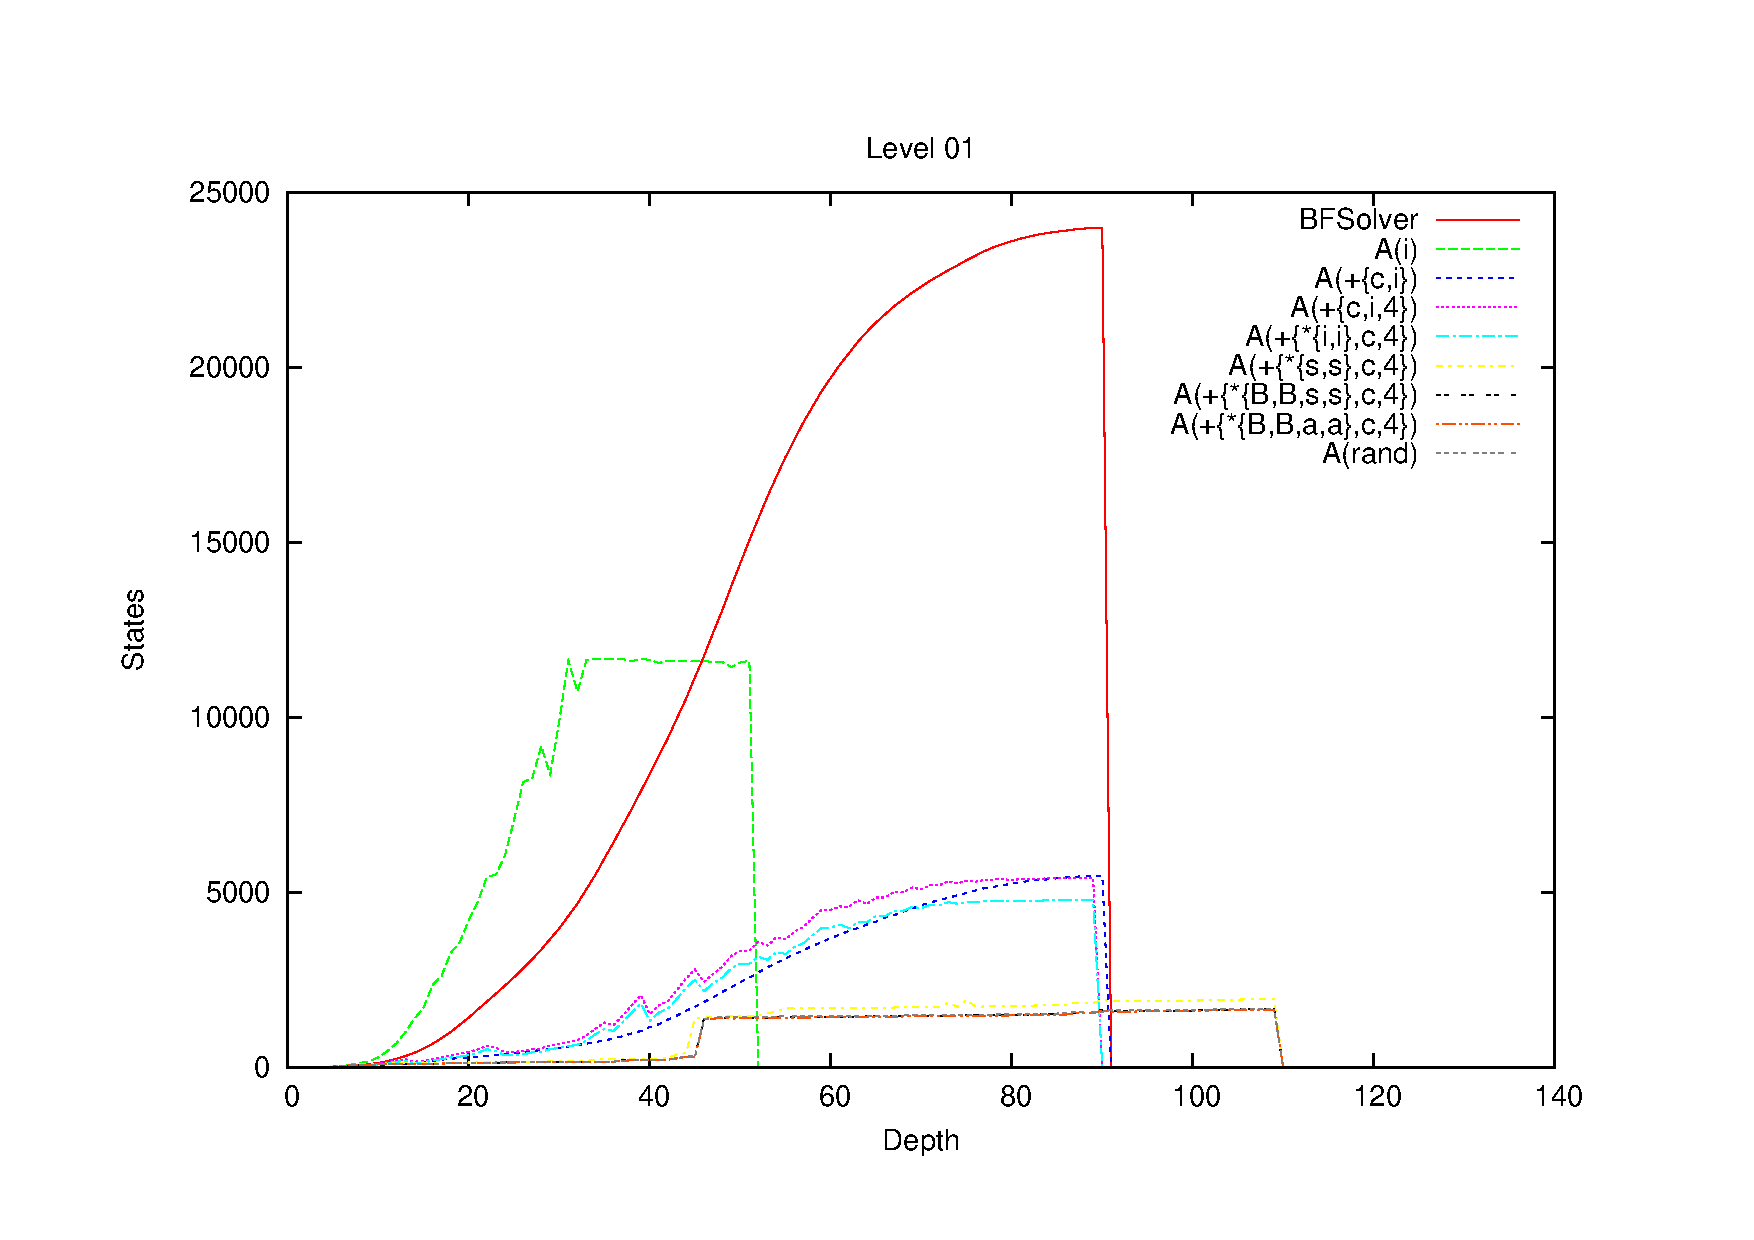
\includegraphics[width=0.85\textwidth]{level01-5}
  \caption{Level 01}
  \label{fig:level01-stats}
\end{figure}
 
\begin{figure}
  \centering
  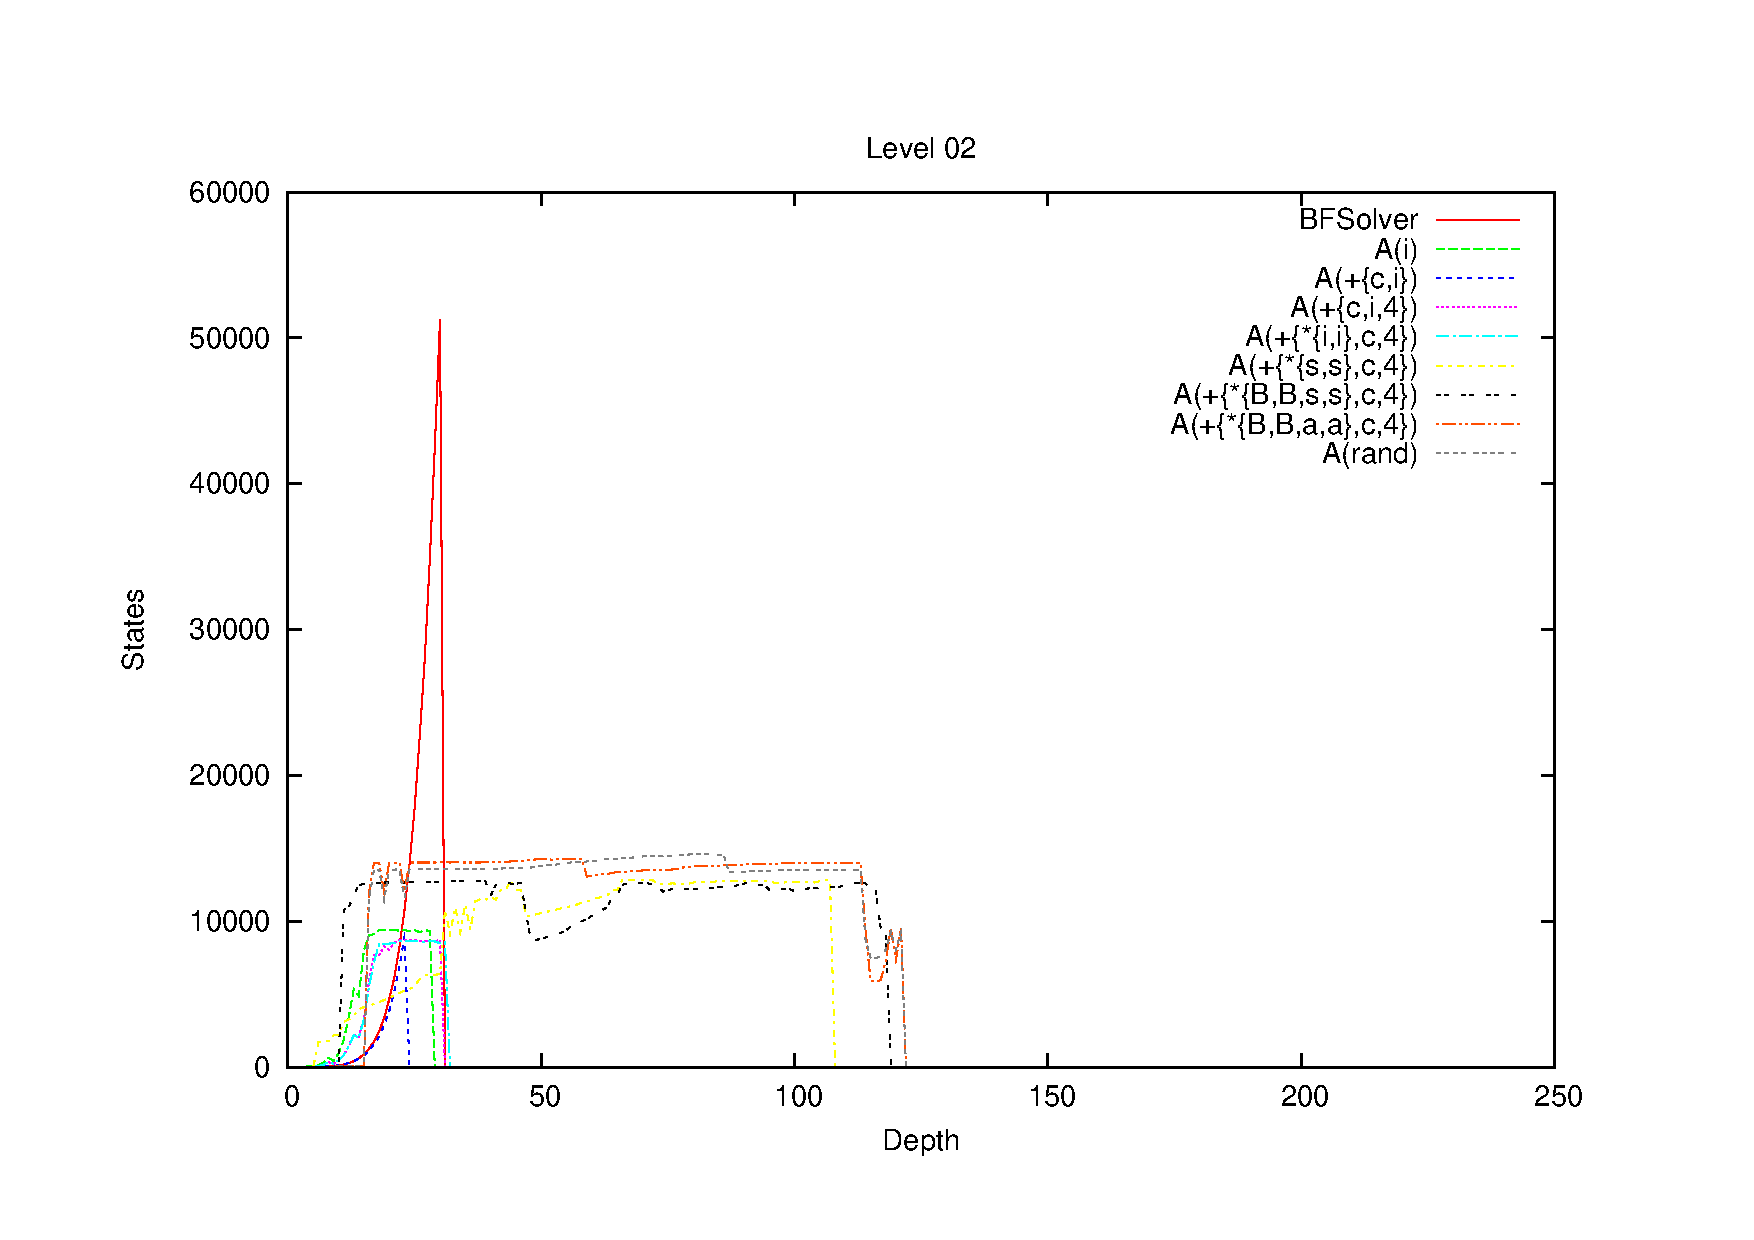
\includegraphics[width=0.85\textwidth]{level02-5}
  \caption{Level 02}
  \label{fig:level02-stats}
\end{figure}

\begin{figure}
  \centering
  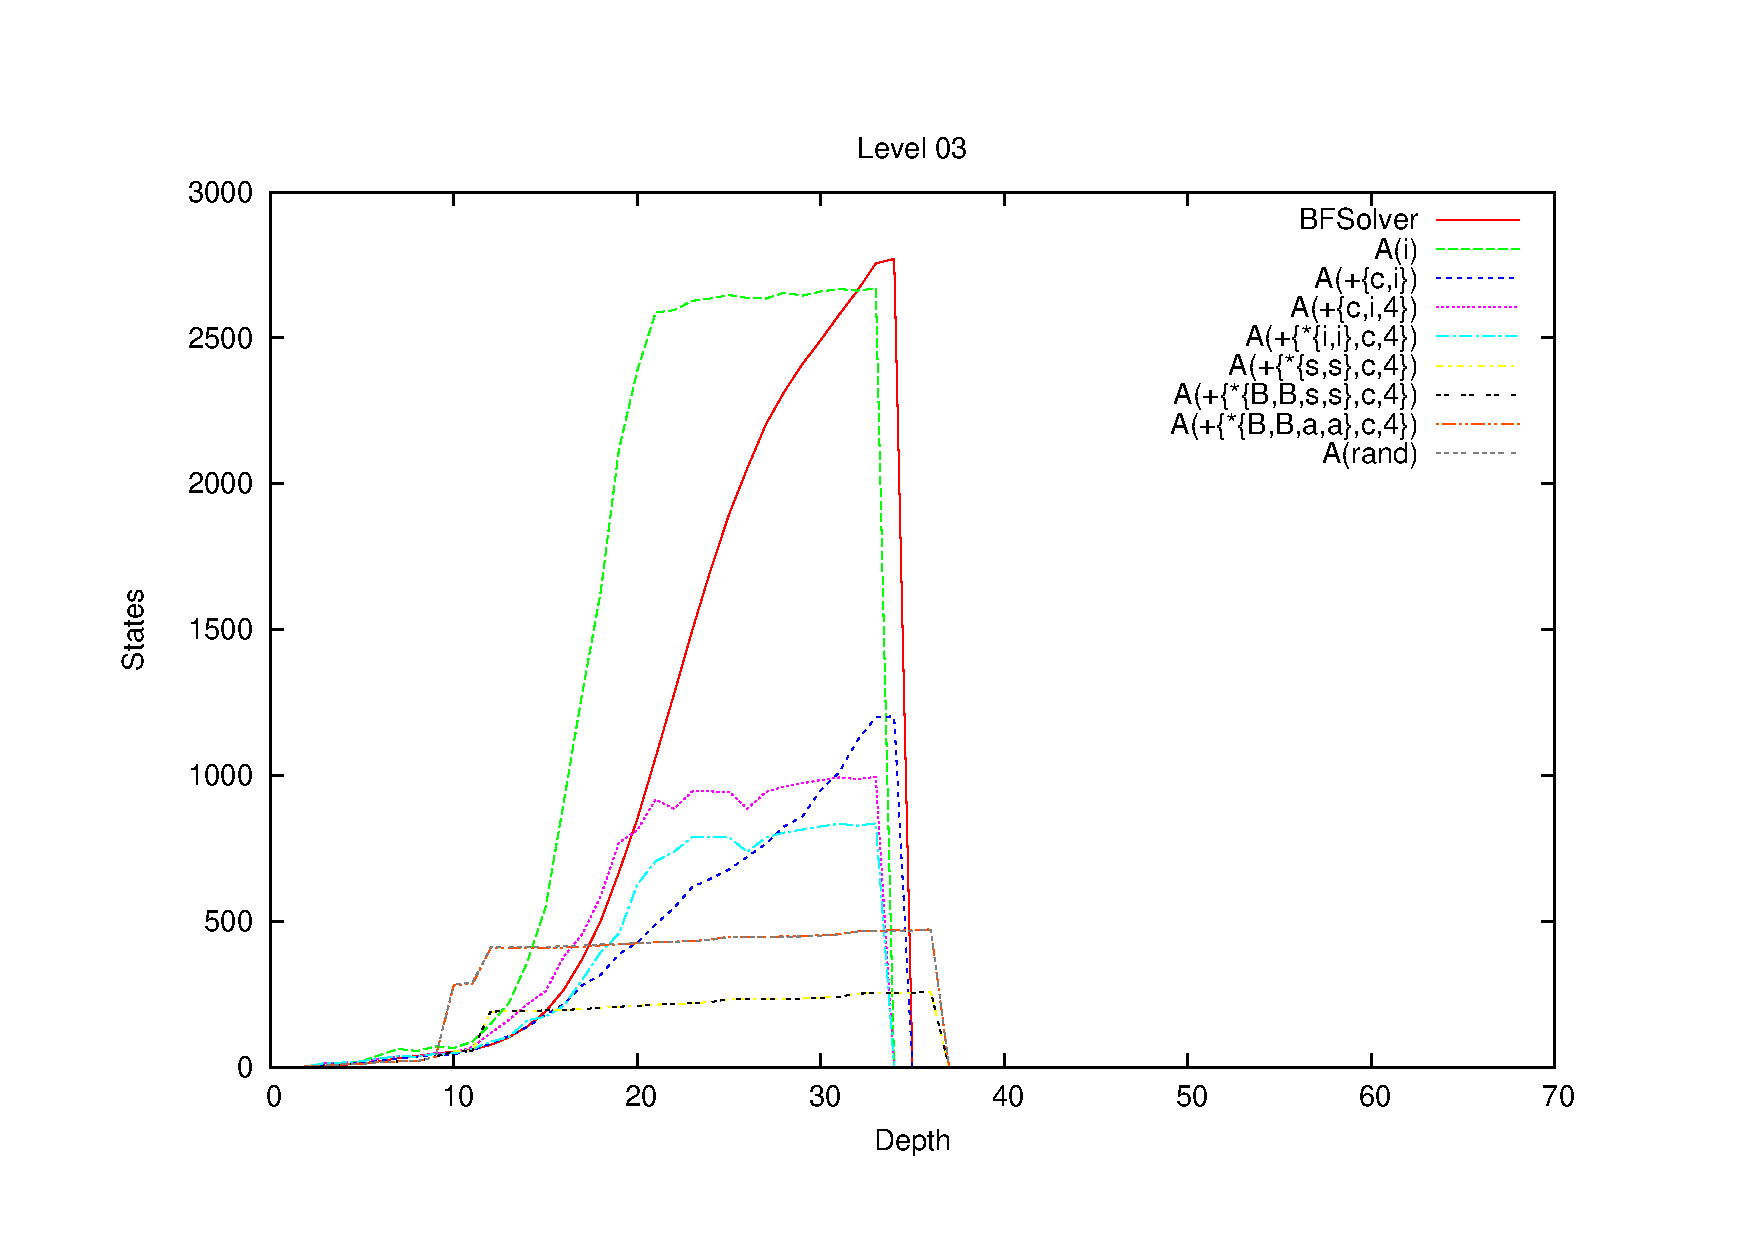
\includegraphics[width=0.85\textwidth]{level03-5}
  \caption{Level 03}
  \label{fig:level03-stats}
\end{figure}
 
\begin{figure}
  \centering
  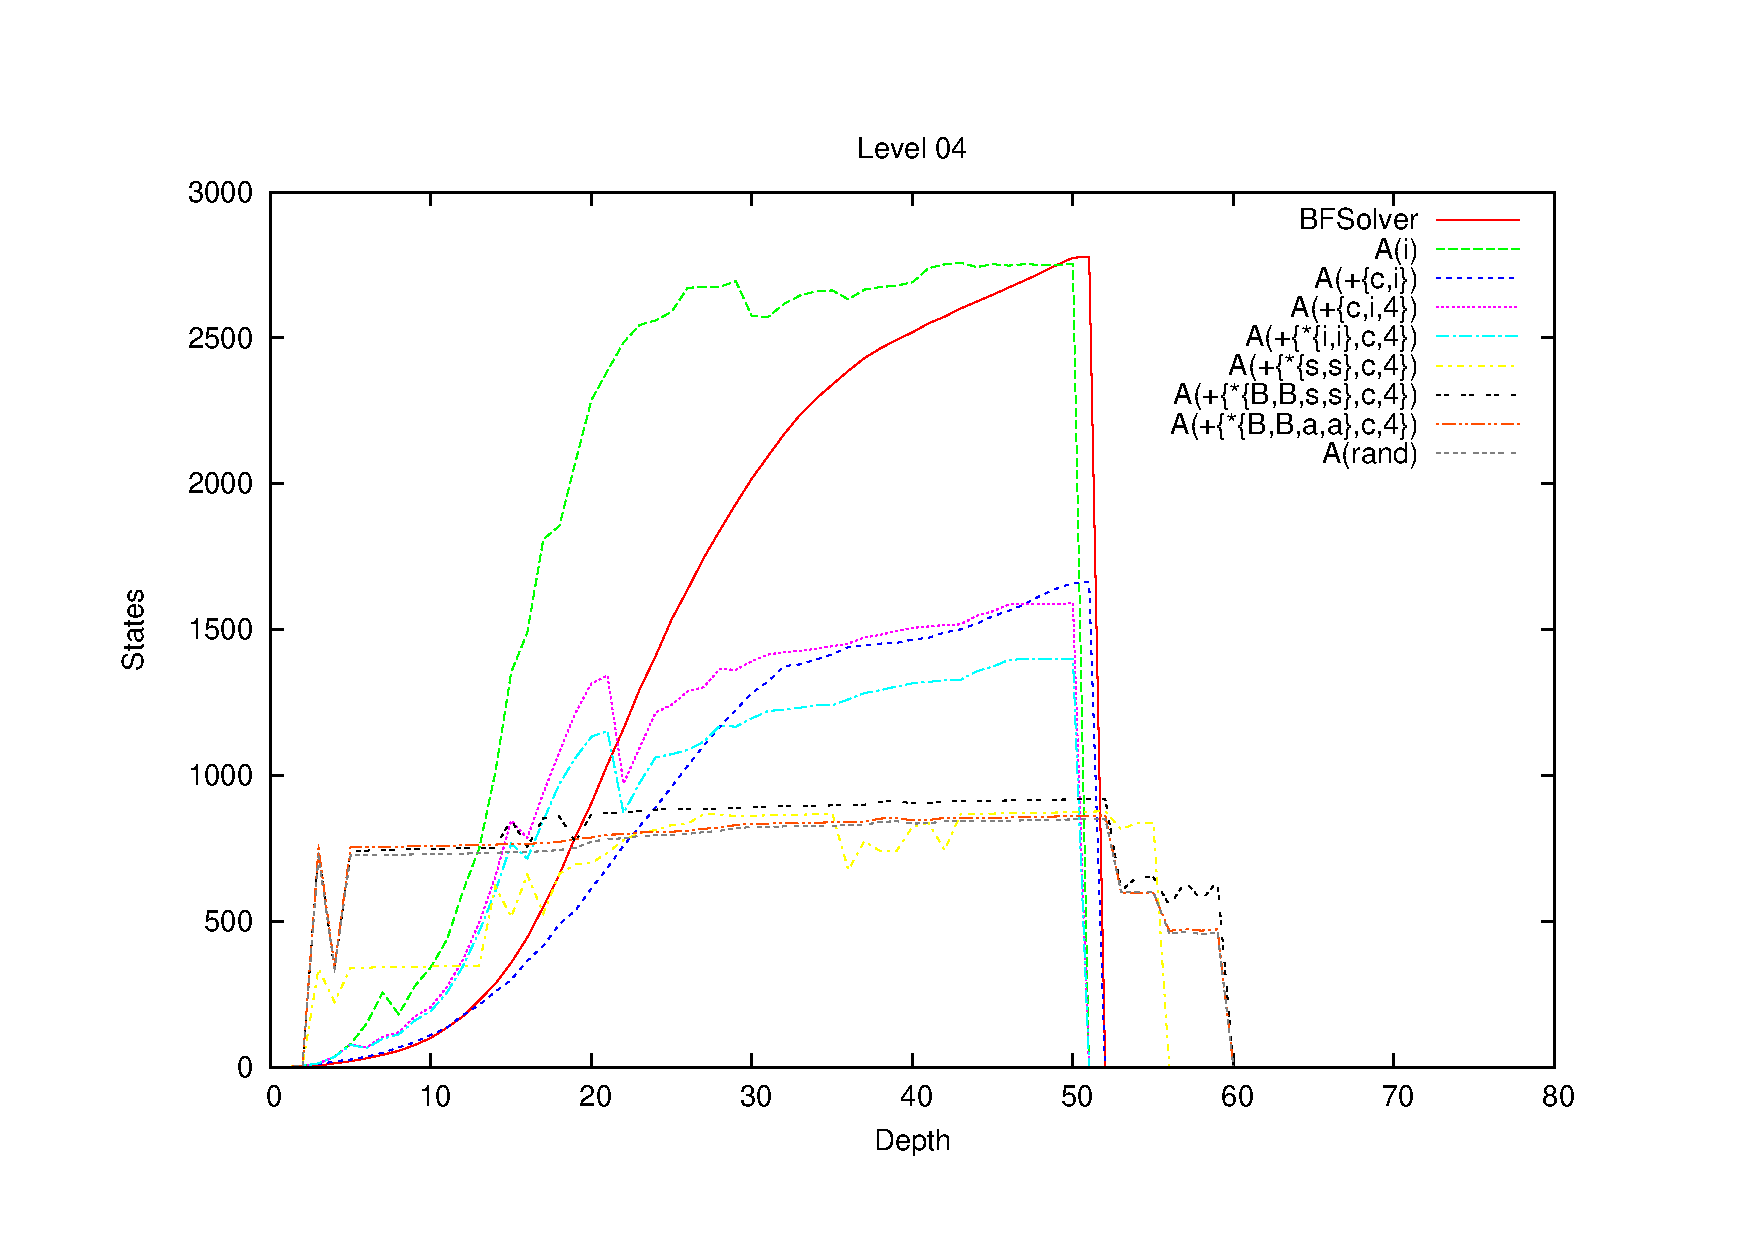
\includegraphics[width=0.85\textwidth]{level04-5}
  \caption{Level 04}
  \label{fig:level04-stats}
\end{figure}

\begin{figure}
  \centering
  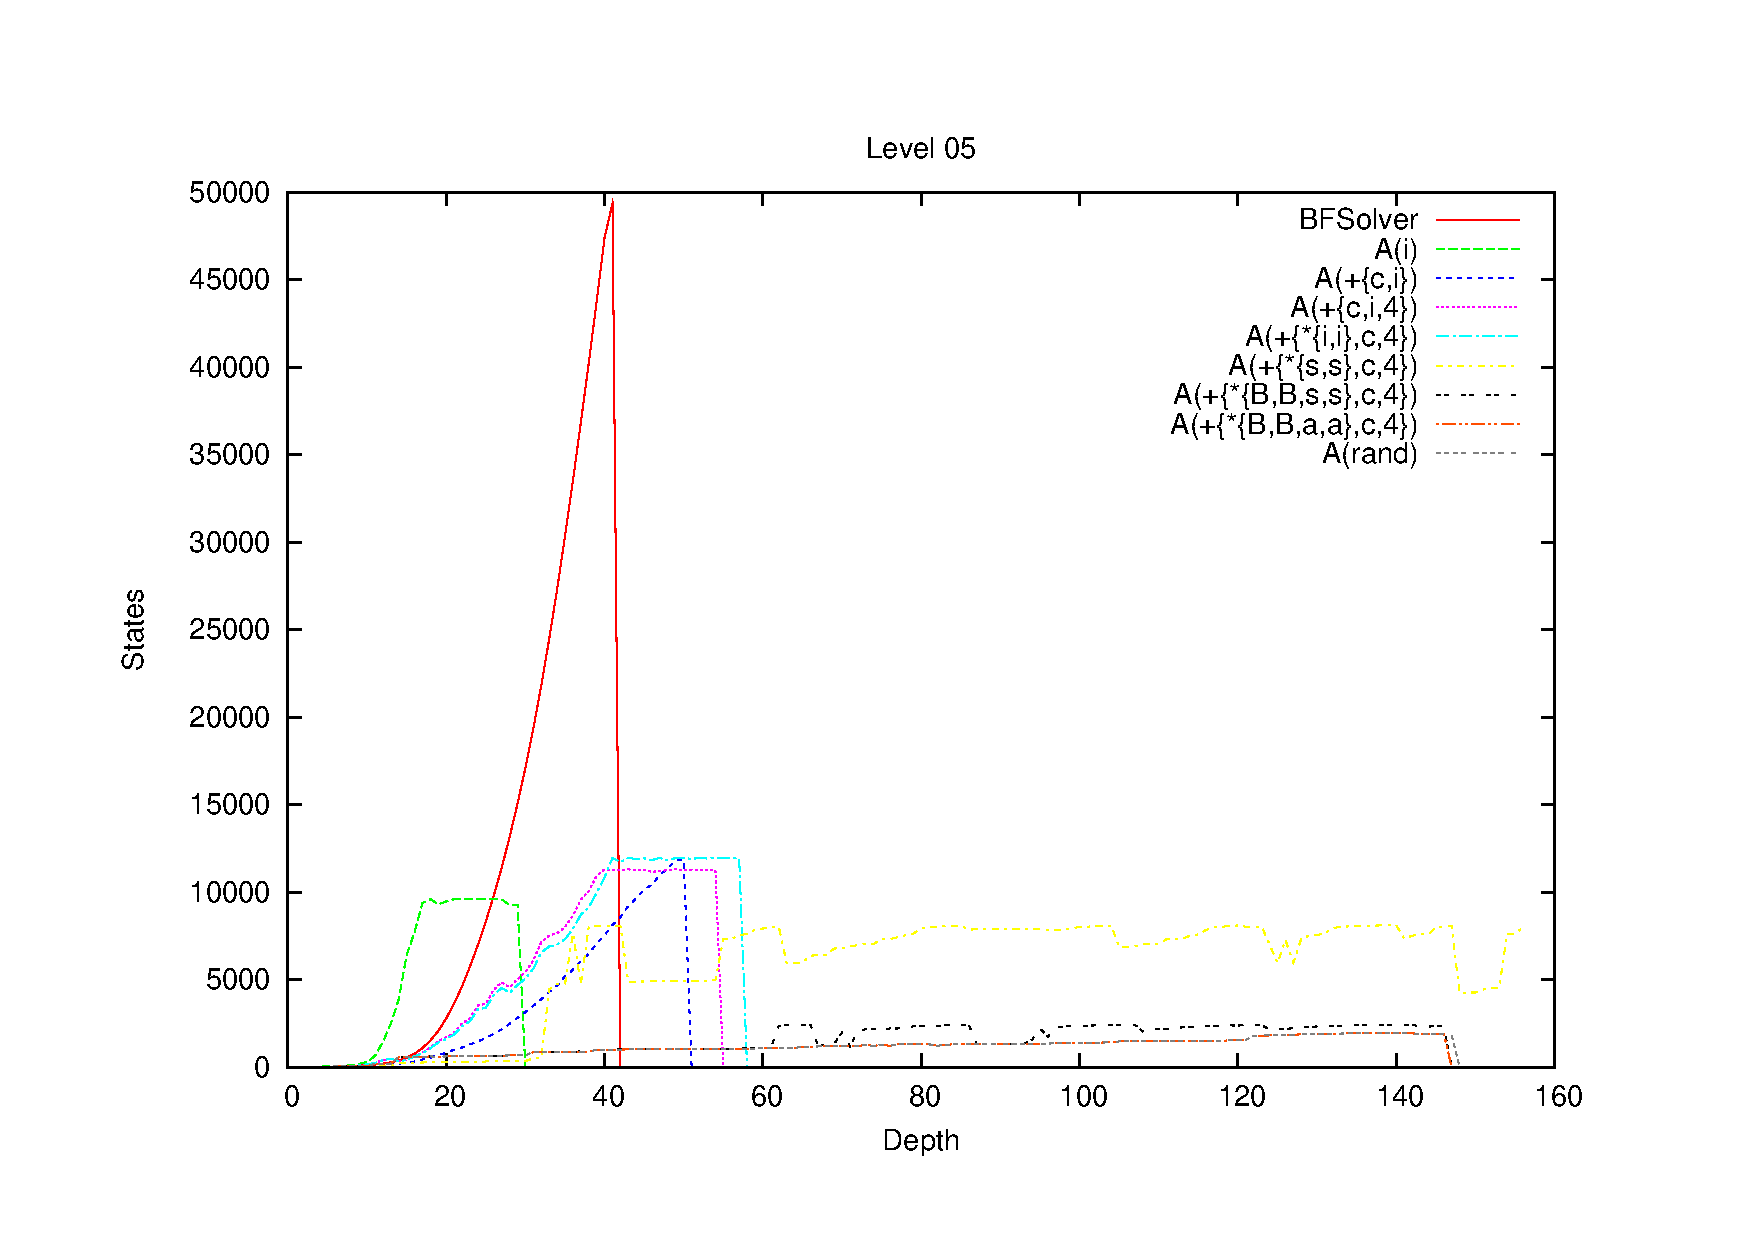
\includegraphics[width=0.85\textwidth]{level05-5}
  \caption{Level 05}
  \label{fig:level05-stats}
\end{figure}
 
\begin{figure}
  \centering
  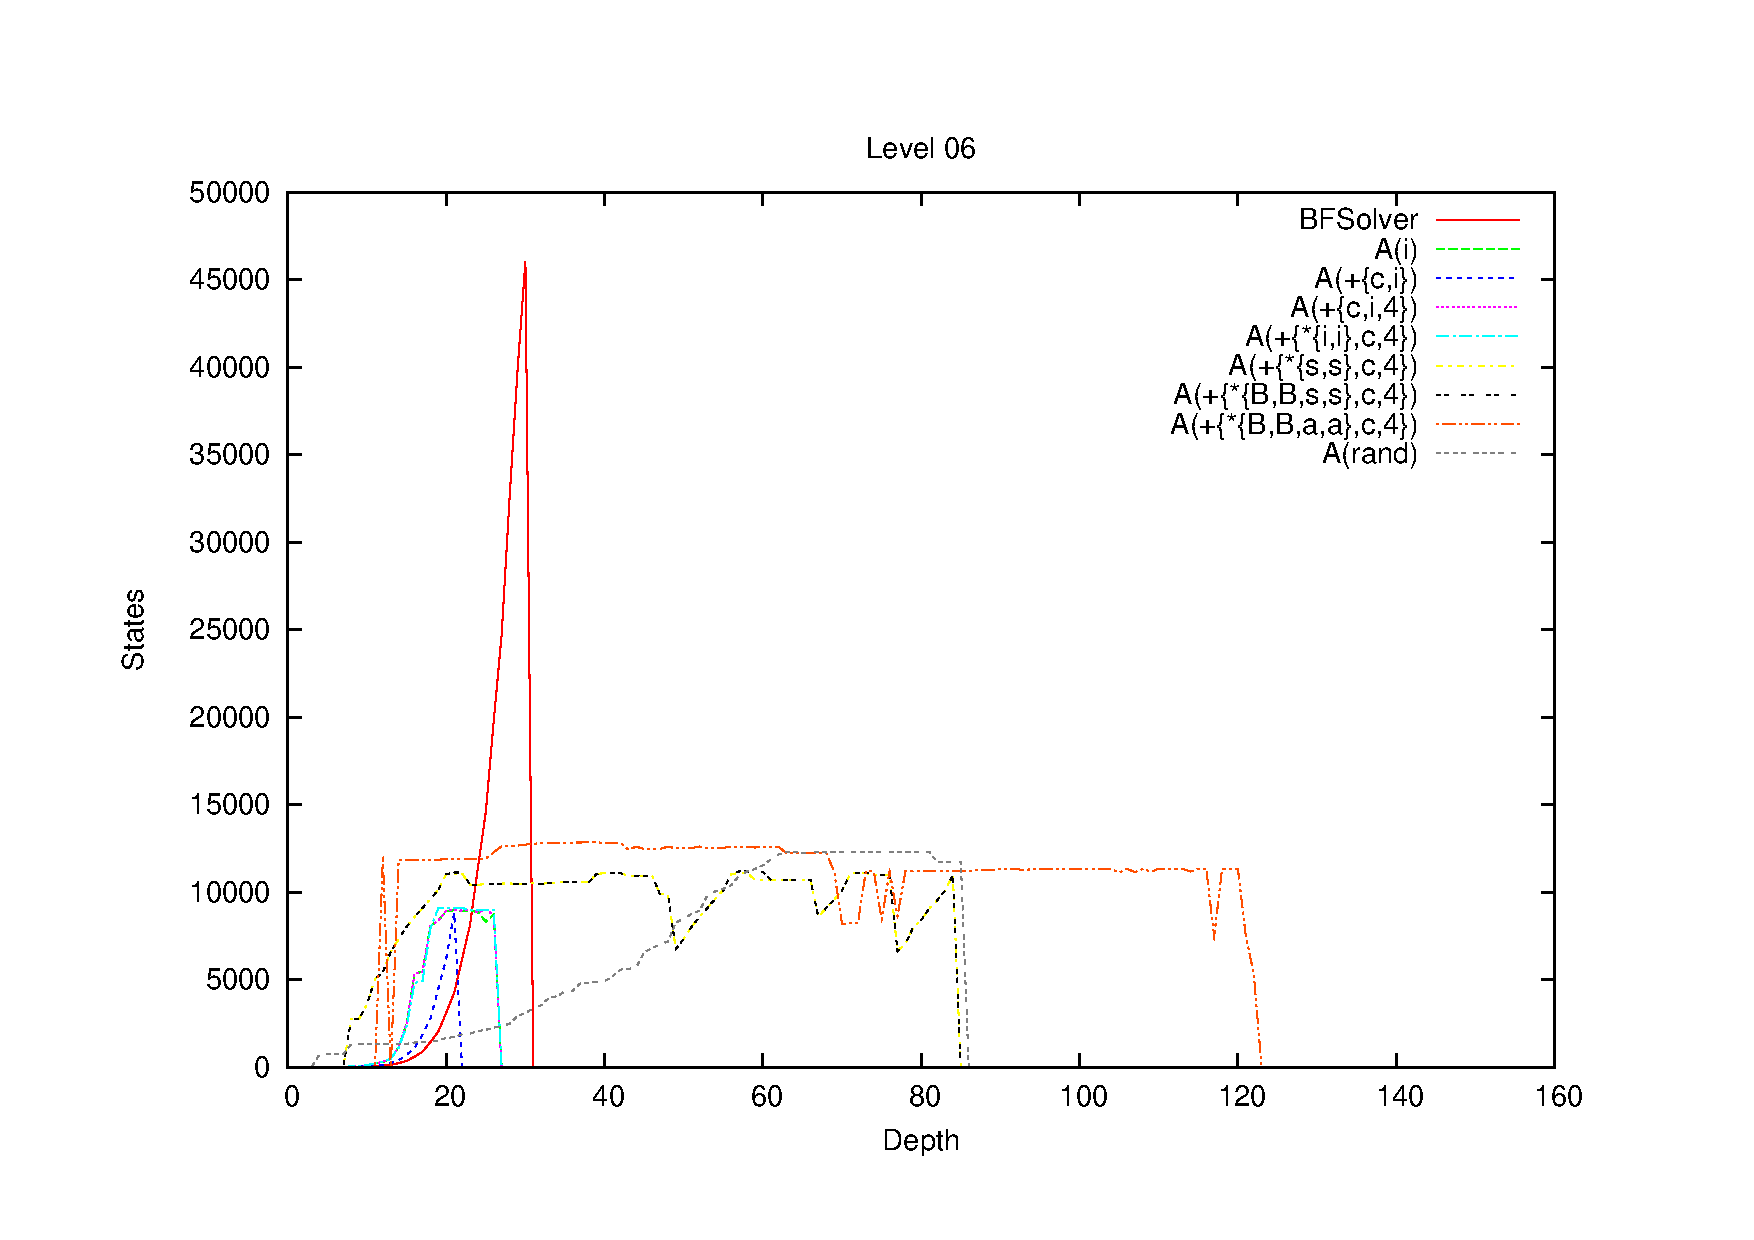
\includegraphics[width=0.85\textwidth]{level06-5}
  \caption{Level 06}
  \label{fig:level06-stats}
\end{figure}

\begin{figure}
  \centering
  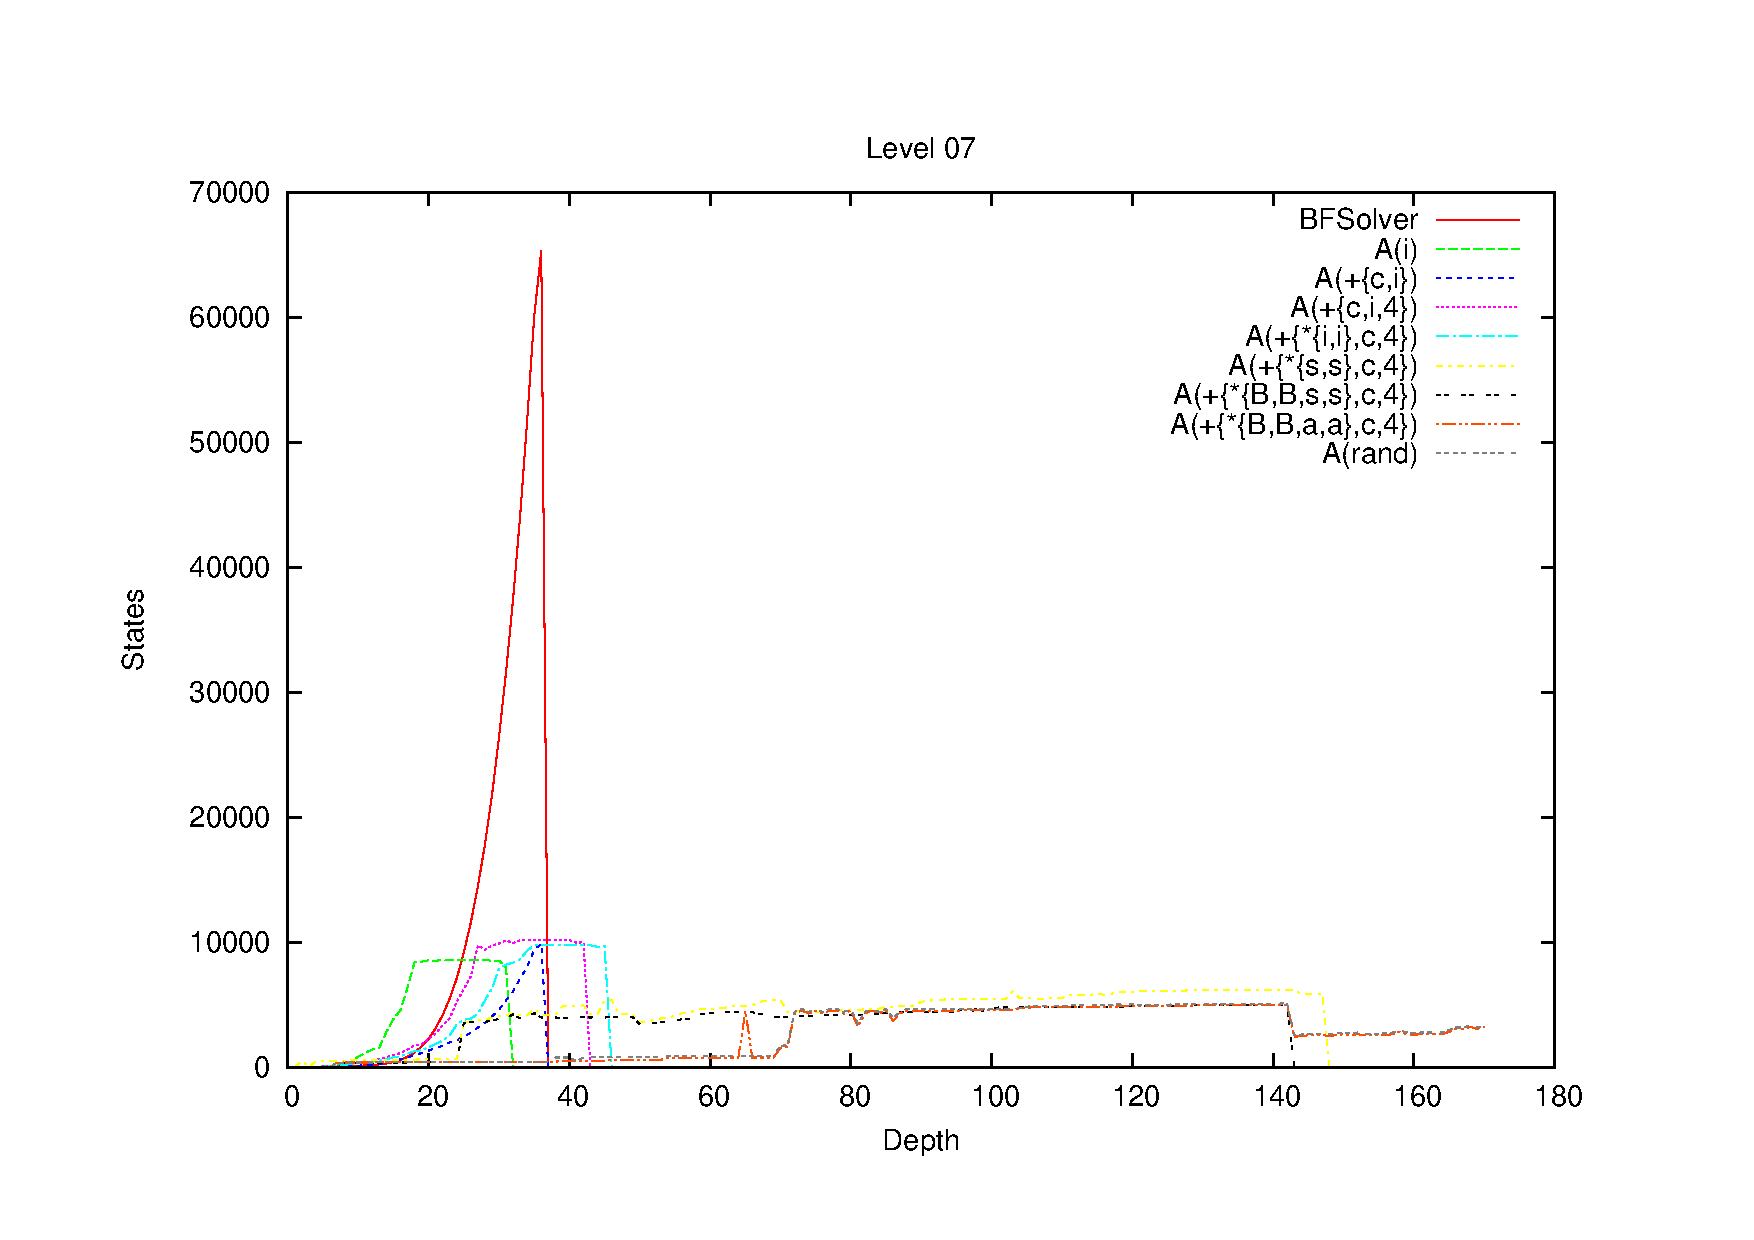
\includegraphics[width=0.85\textwidth]{level07-5}
  \caption{Level 07}
  \label{fig:level07-stats}
\end{figure}
 
\begin{figure}
  \centering
  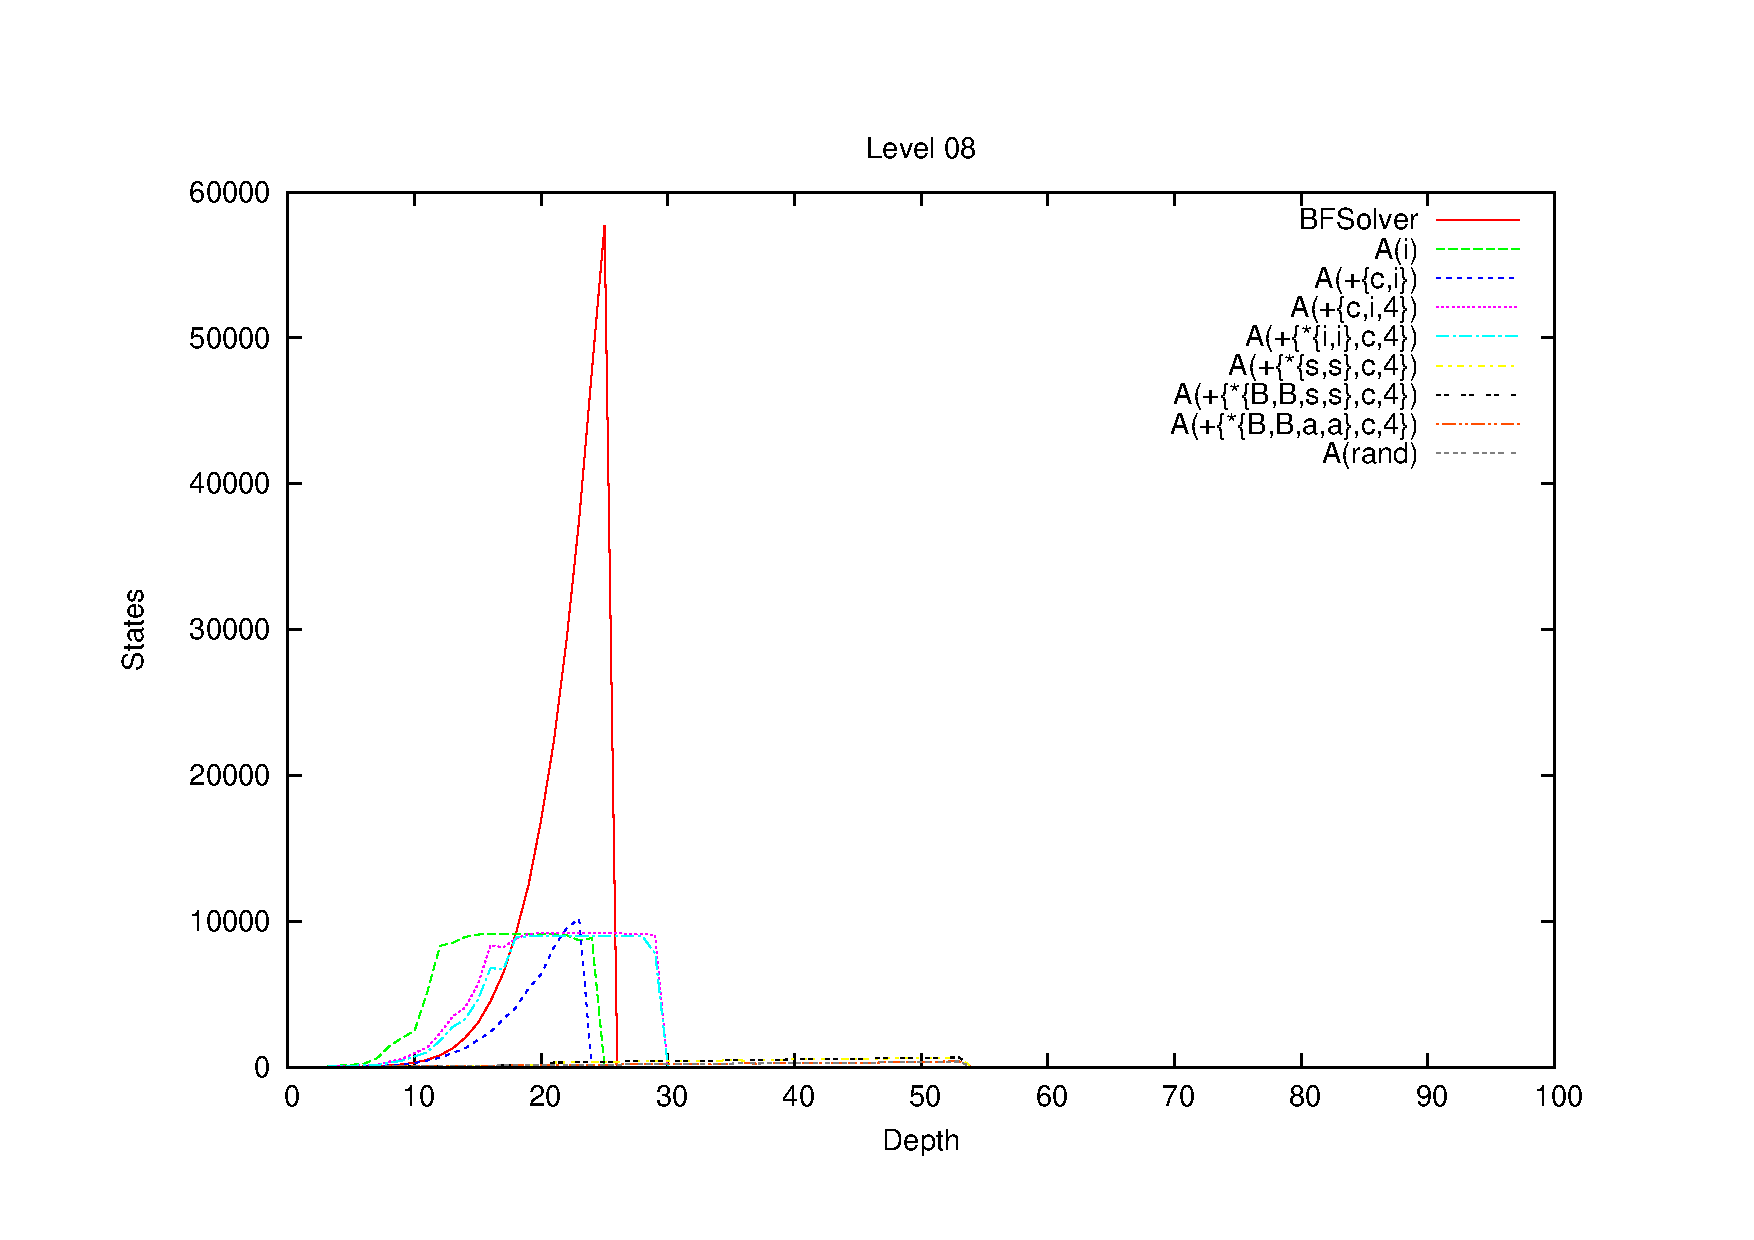
\includegraphics[width=0.85\textwidth]{level08-5}
  \caption{Level 08}
  \label{fig:level08-stats}
\end{figure}

\begin{figure}
  \centering
  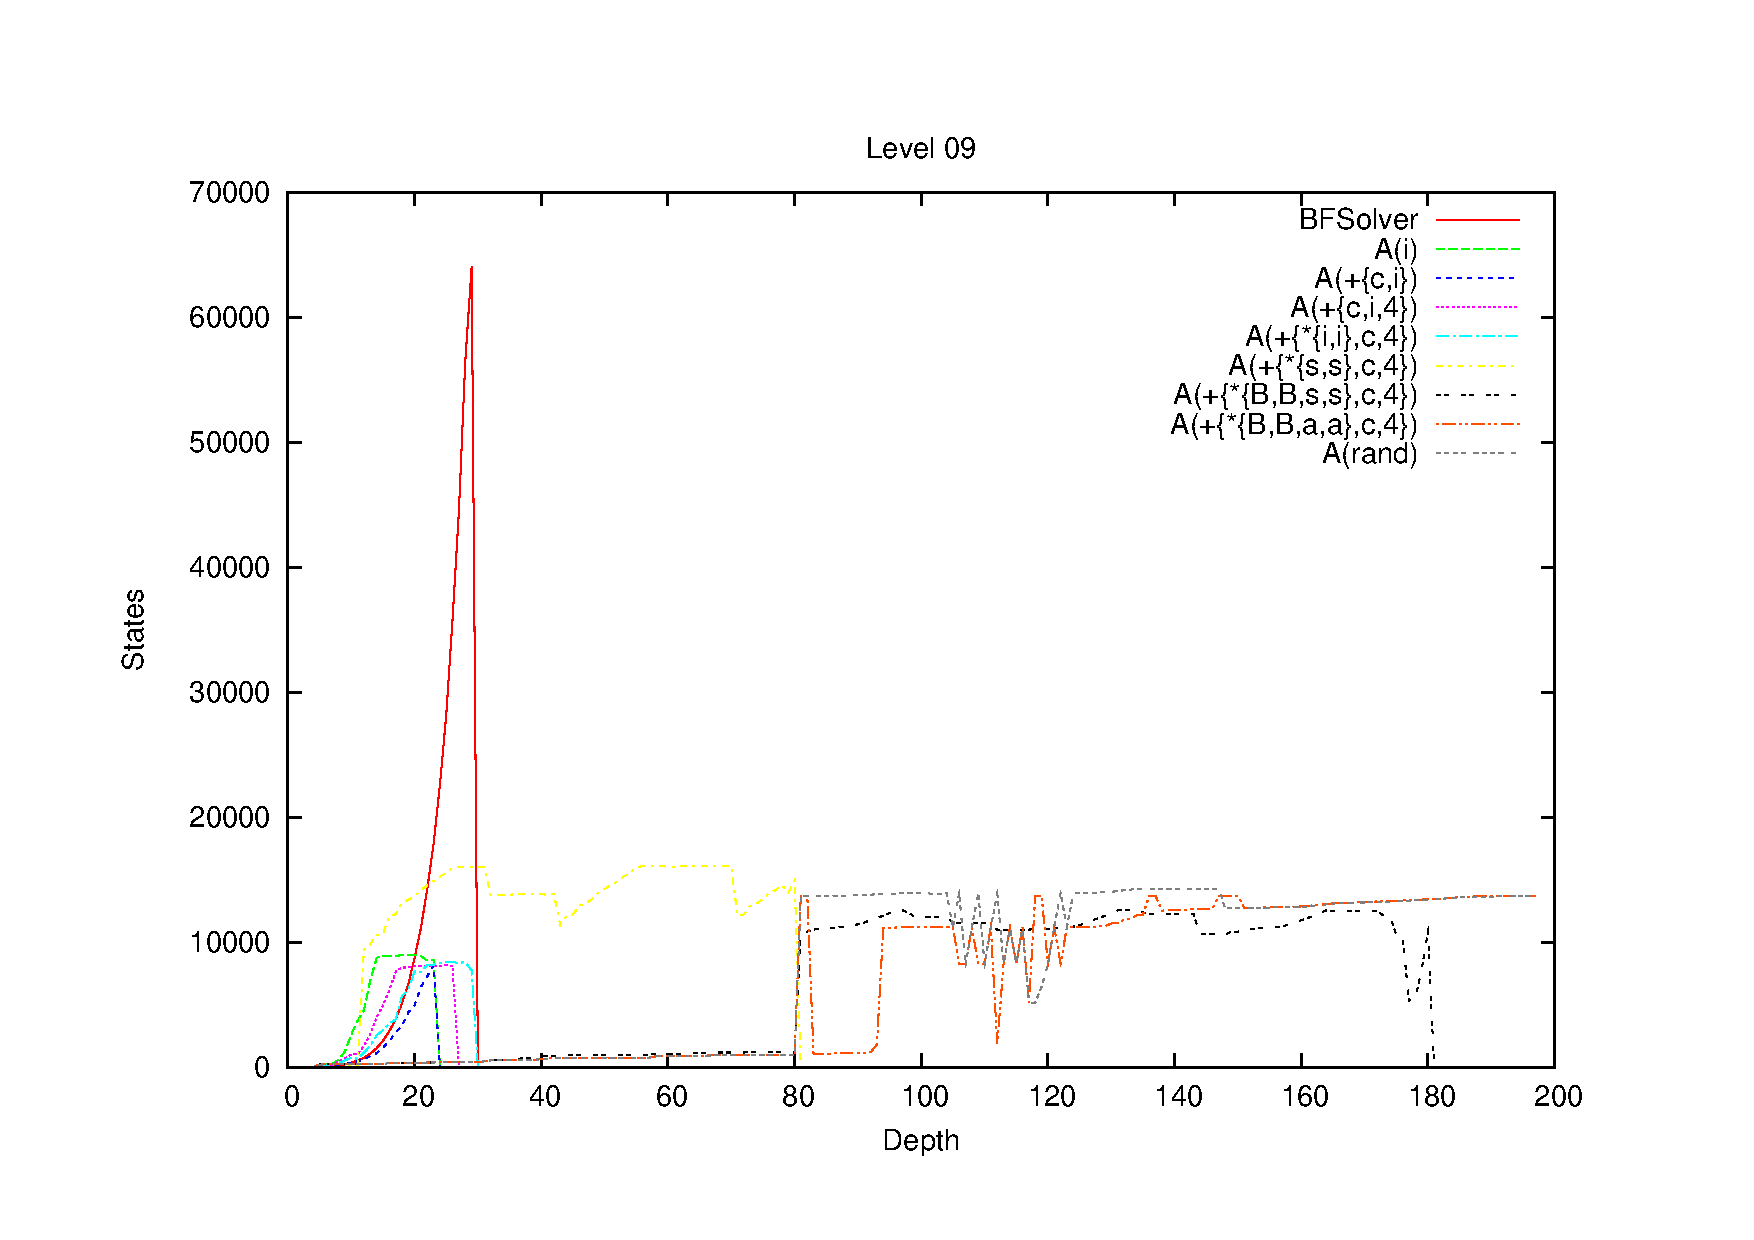
\includegraphics[width=0.85\textwidth]{level09-5}
  \caption{Level 09}
  \label{fig:level09-stats}
\end{figure}
 
\begin{figure}
  \centering
  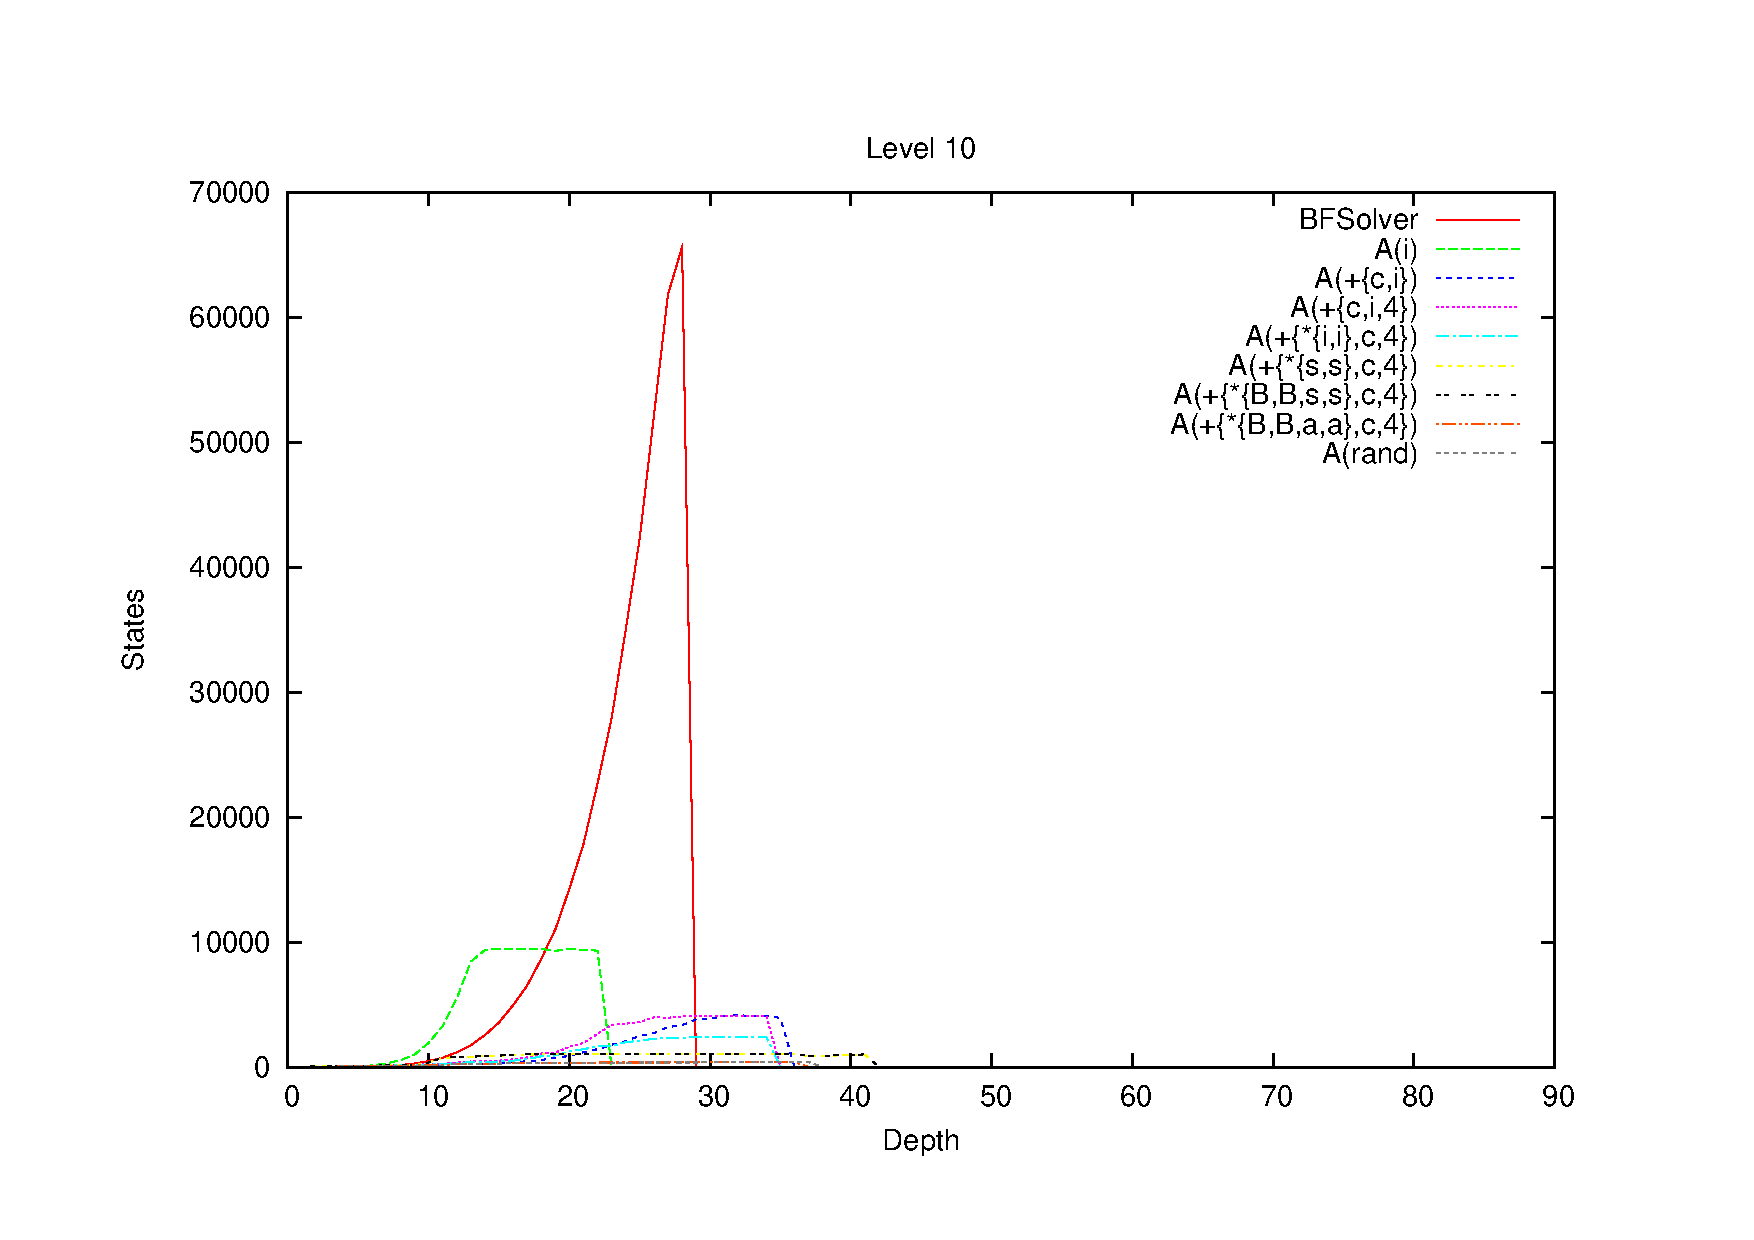
\includegraphics[width=0.85\textwidth]{level10-5}
  \caption{Level 10}
  \label{fig:level10-stats}
\end{figure}

\clearpage

\begin{figure}
  \centering
  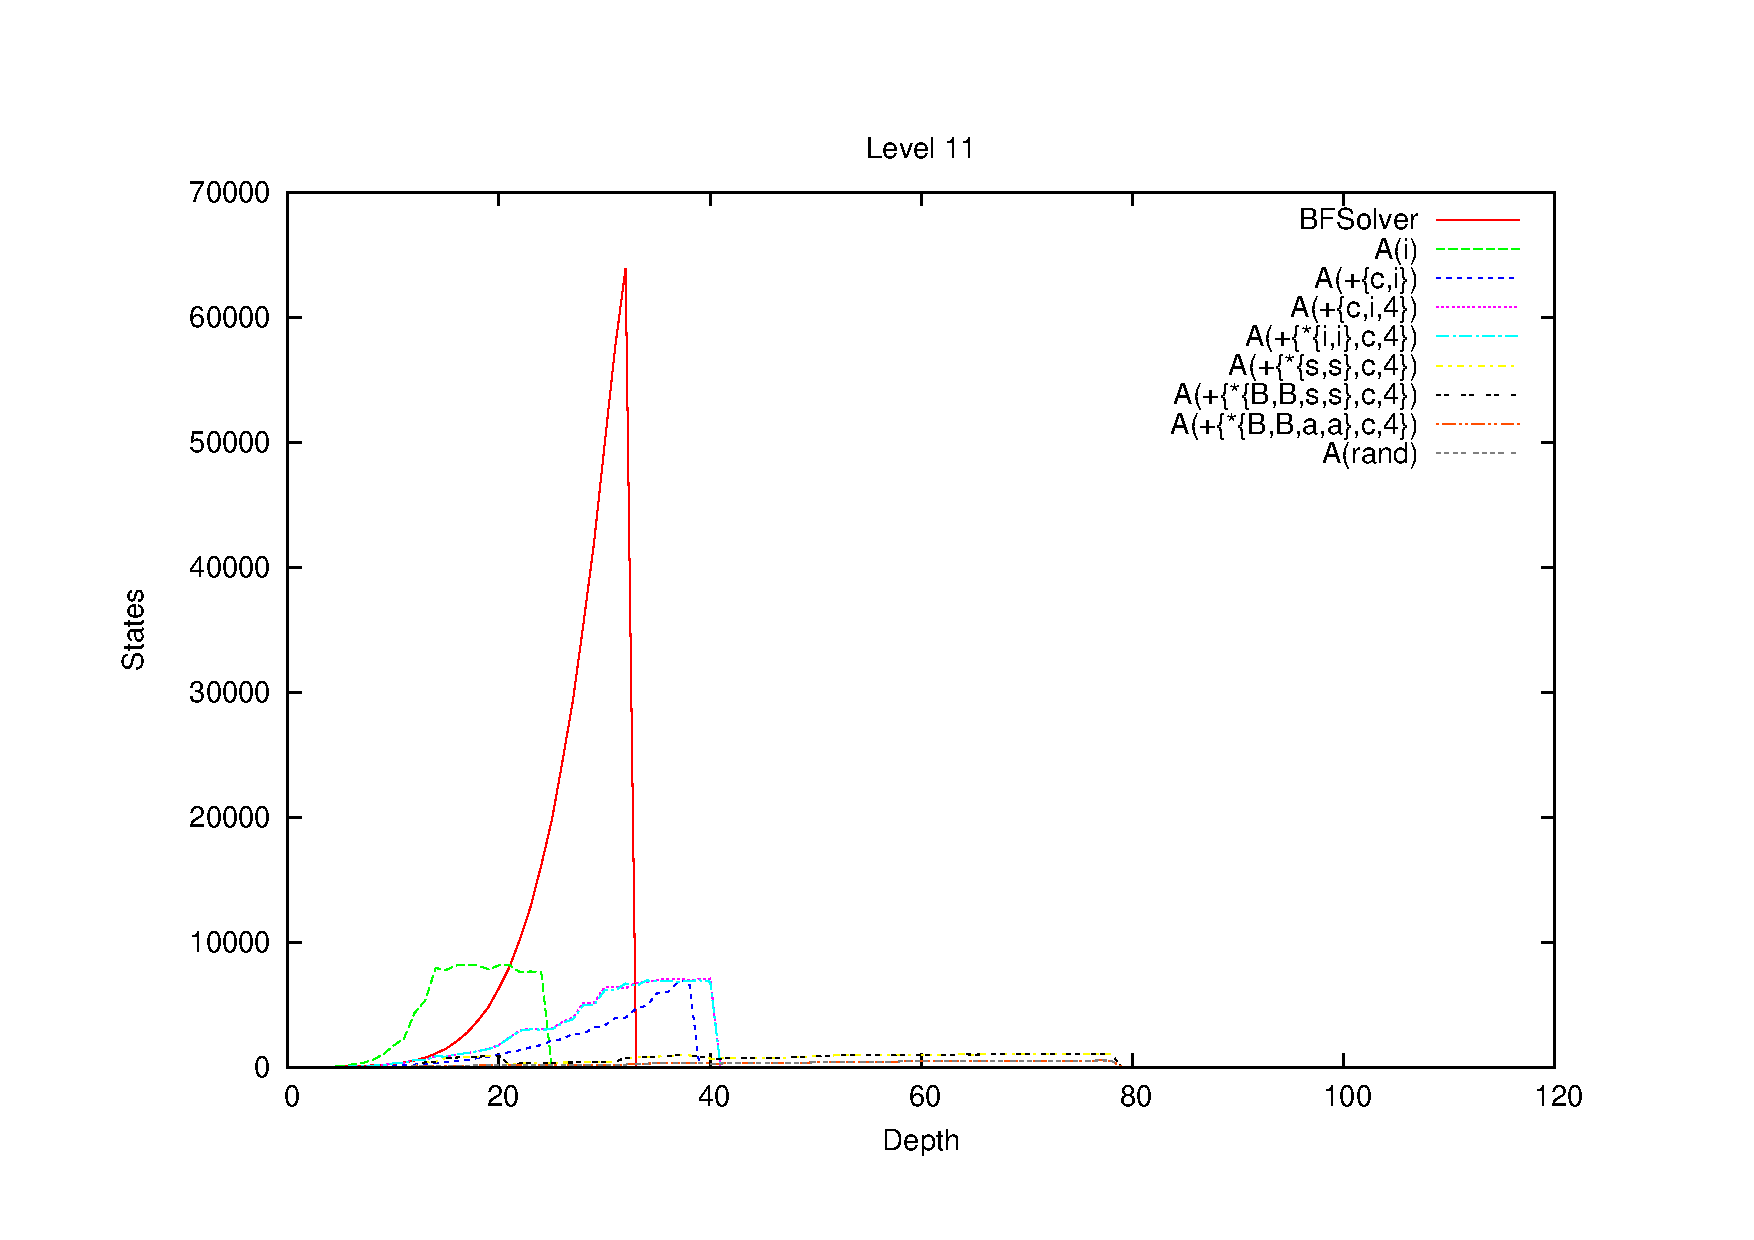
\includegraphics[width=0.85\textwidth]{level11-5}
  \caption{Level 11}
  \label{fig:level11-stats}
\end{figure}
 
\begin{figure}
  \centering
  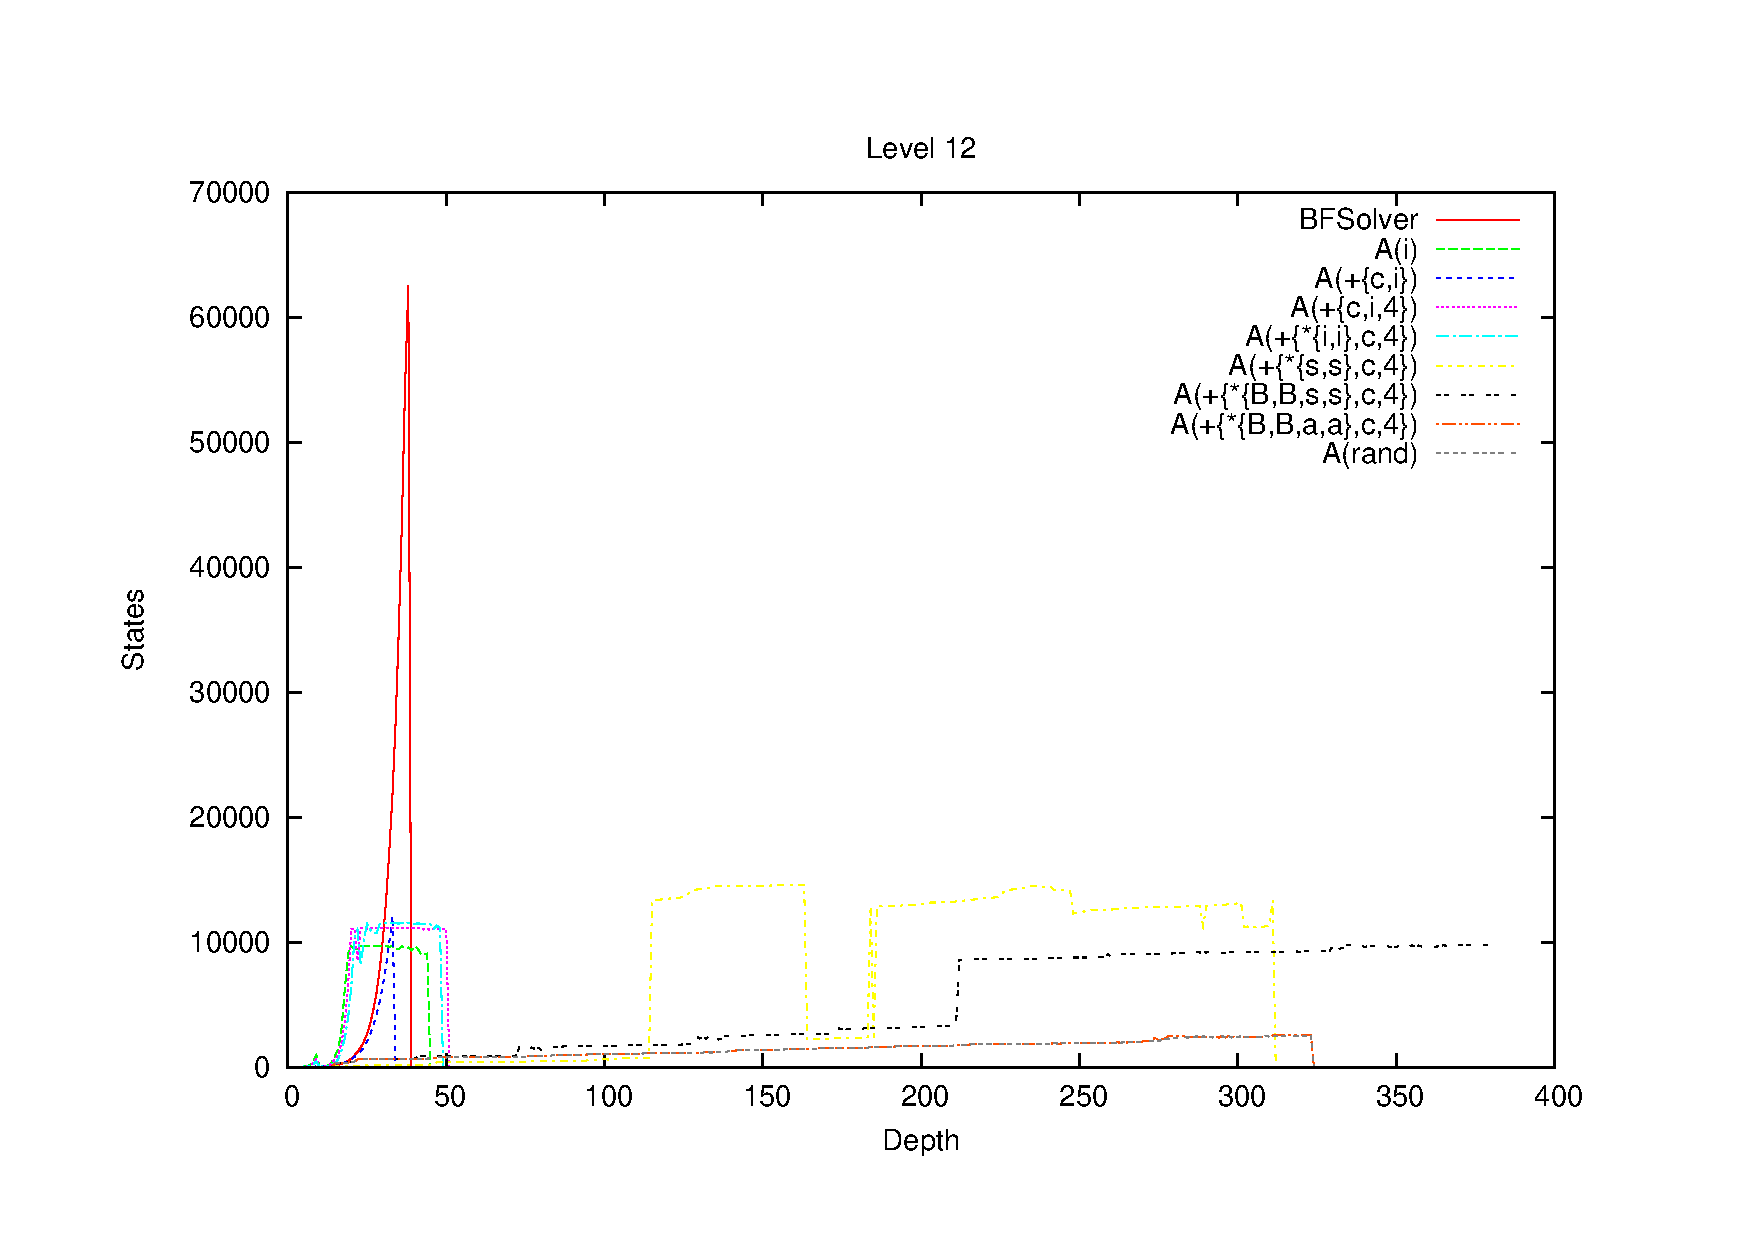
\includegraphics[width=0.85\textwidth]{level12-5}
  \caption{Level 12}
  \label{fig:level12-stats}
\end{figure}

\begin{figure}
  \centering
  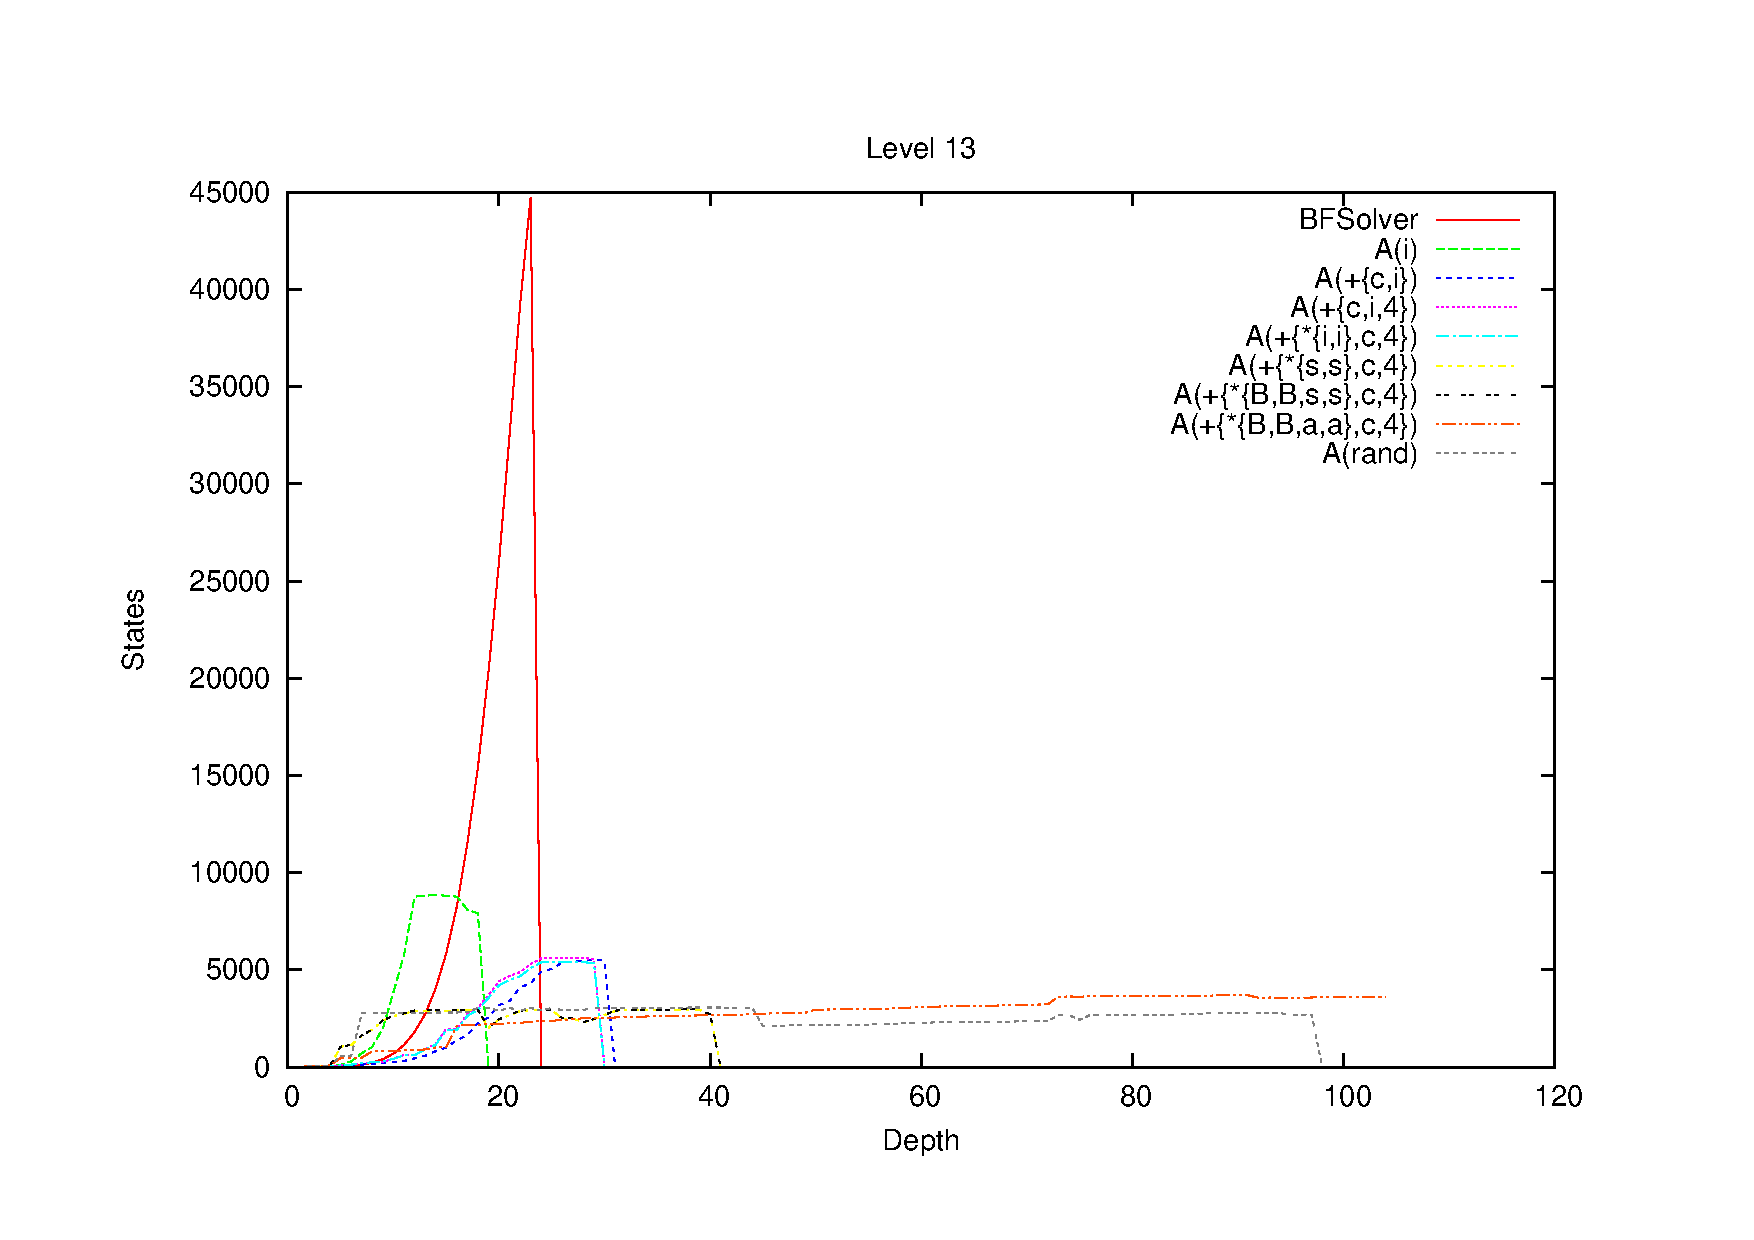
\includegraphics[width=0.85\textwidth]{level13-5}
  \caption{Level 13}
  \label{fig:level13-stats}
\end{figure}

\begin{figure}
  \centering
  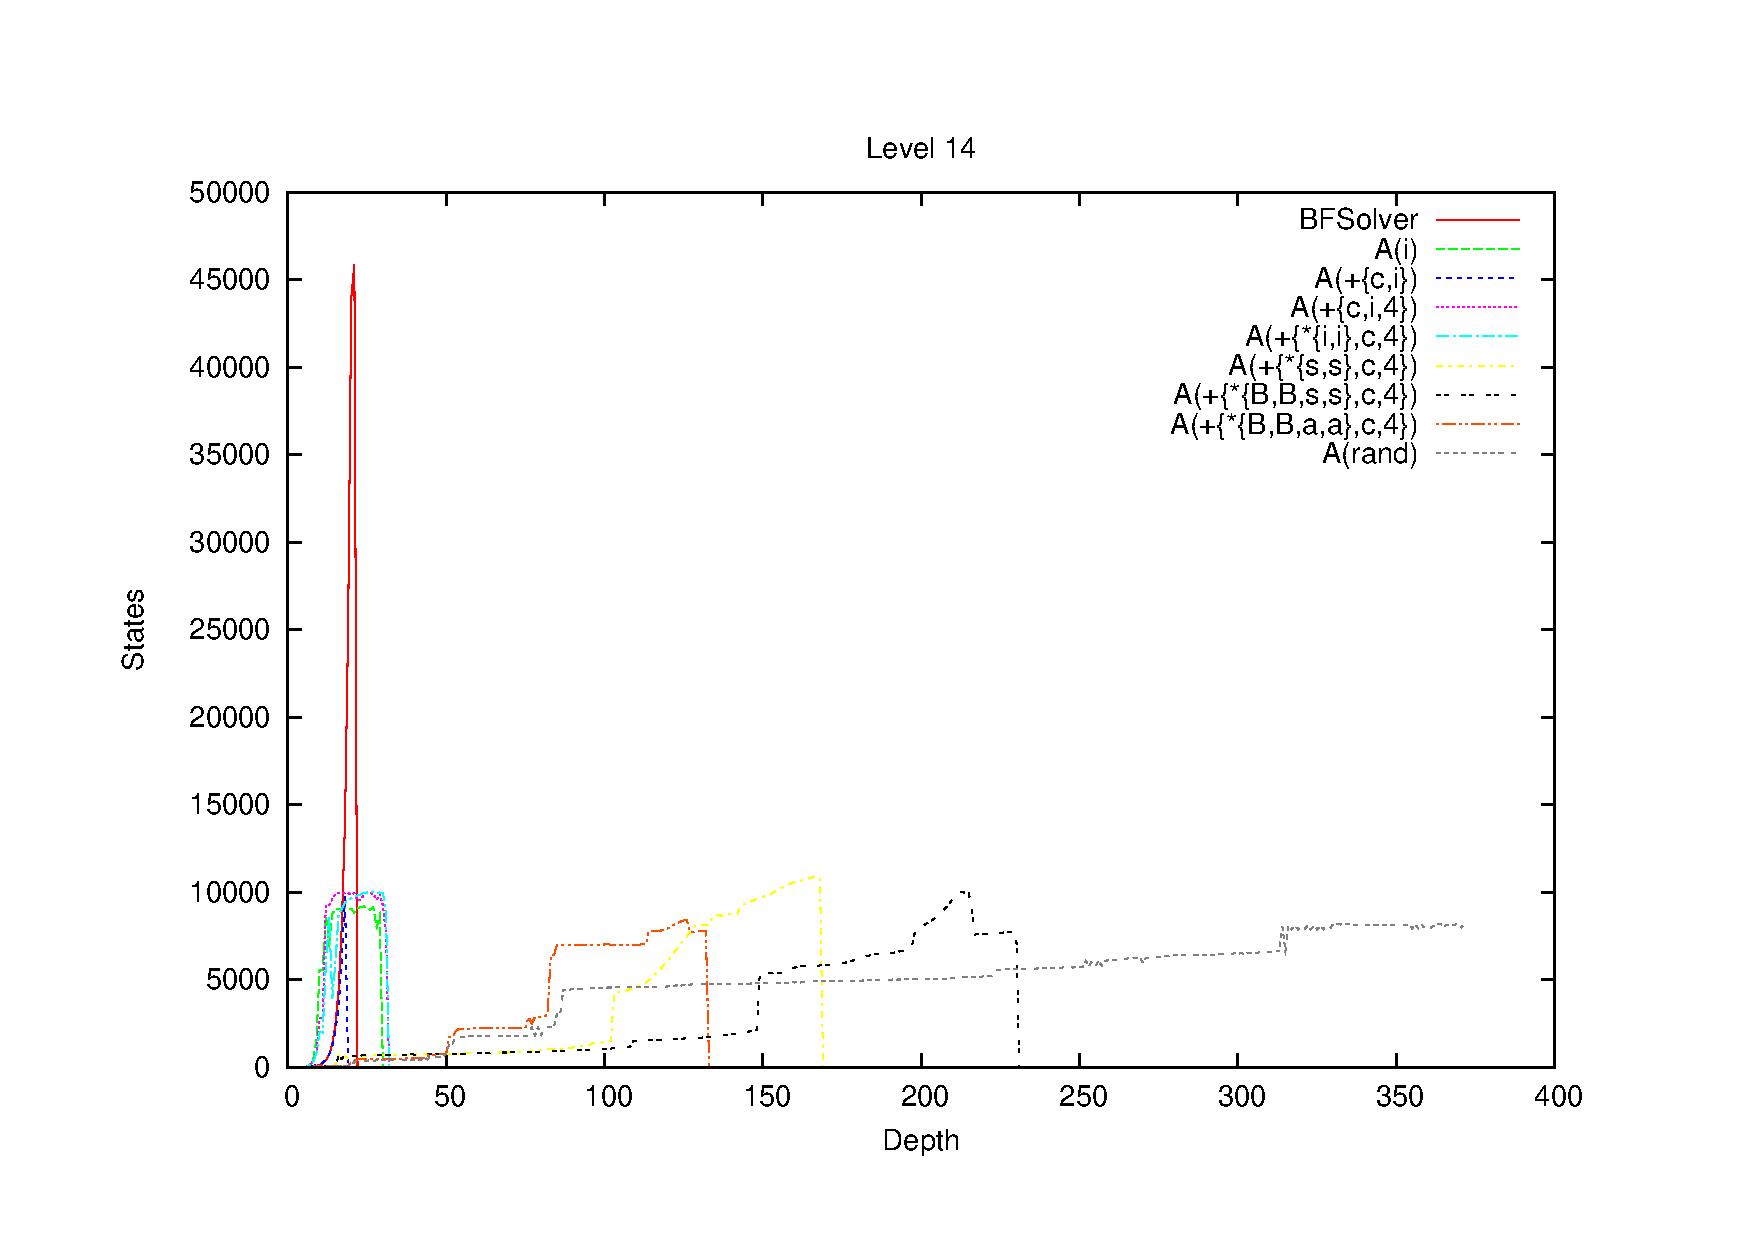
\includegraphics[width=0.85\textwidth]{level14-5}
  \caption{Level 14}
  \label{fig:level14-stats}
\end{figure}
 
\begin{figure}
  \centering
  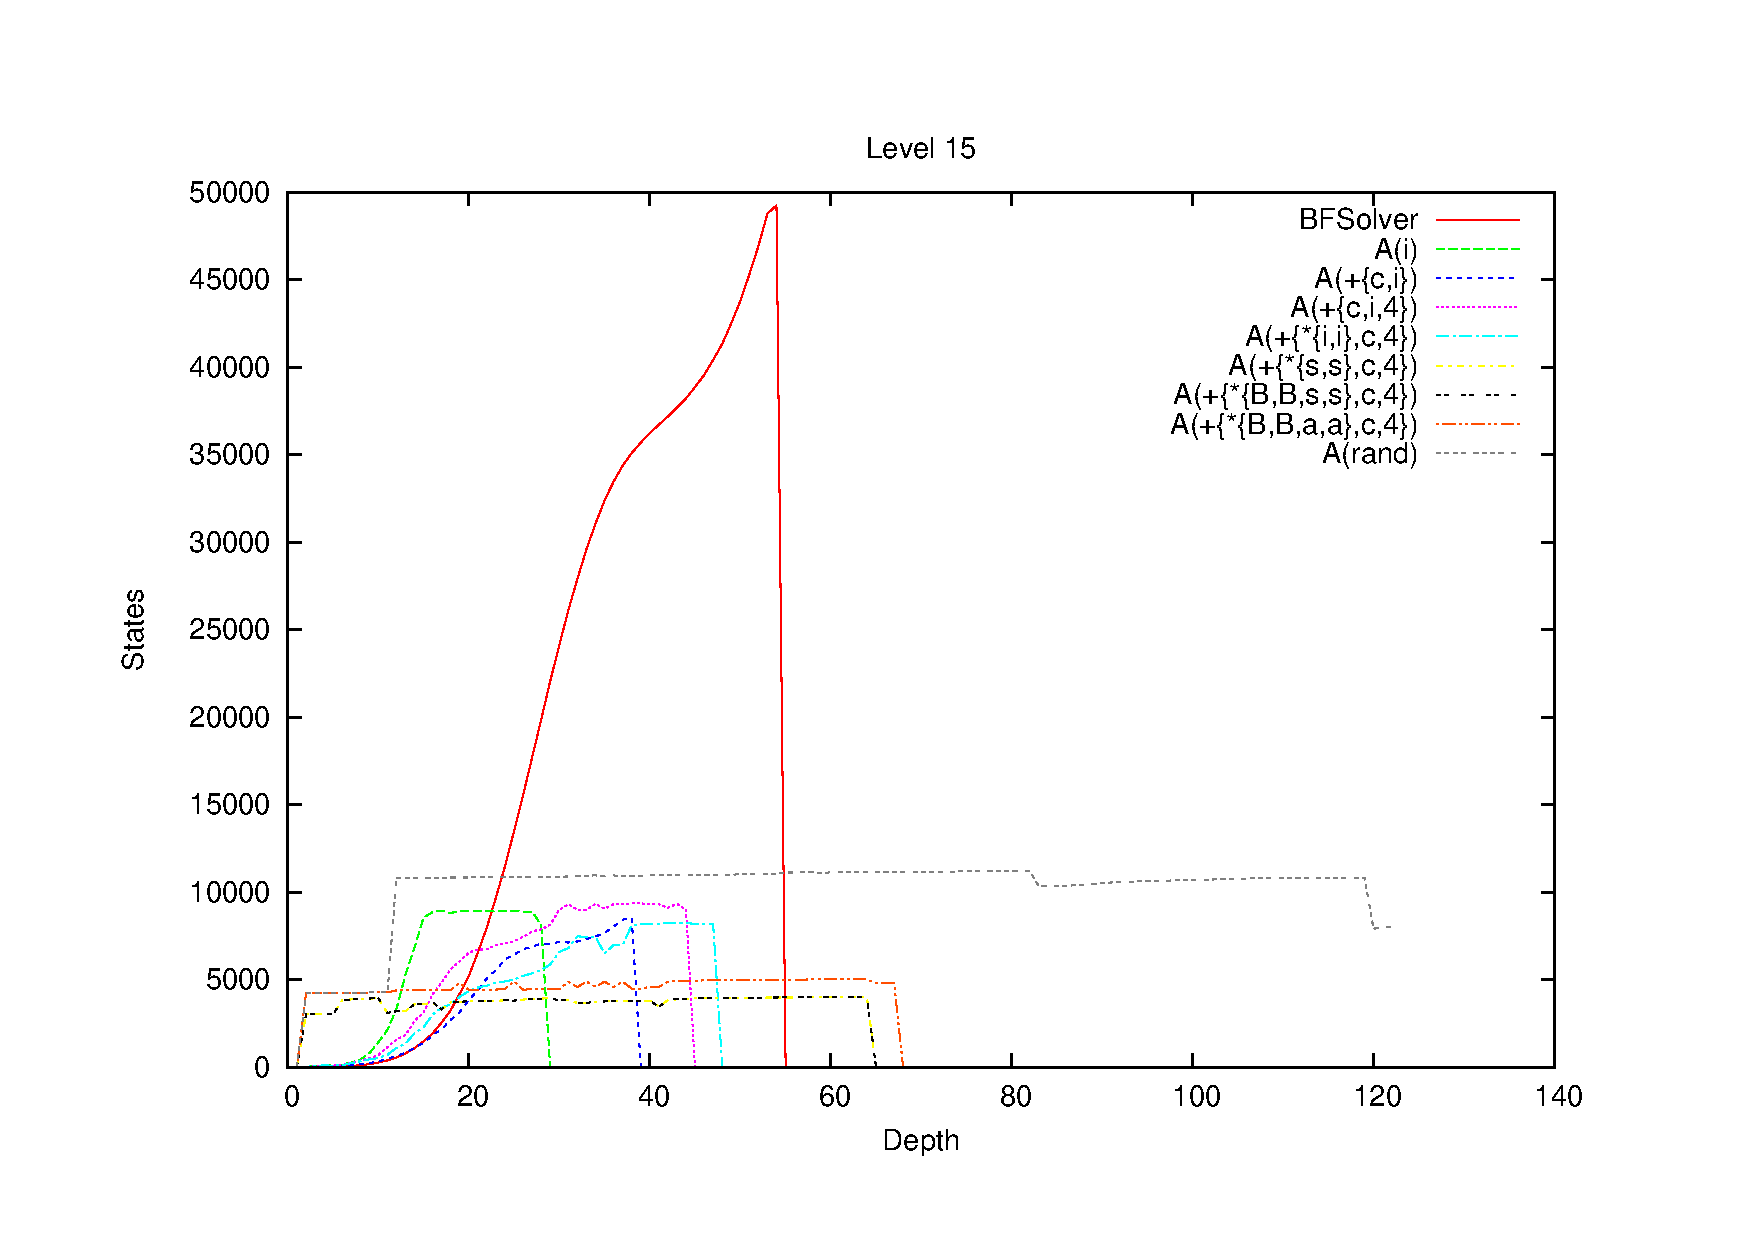
\includegraphics[width=0.85\textwidth]{level15-5}
  \caption{Level 15}
  \label{fig:level15-stats}
\end{figure}

\begin{figure}
  \centering
  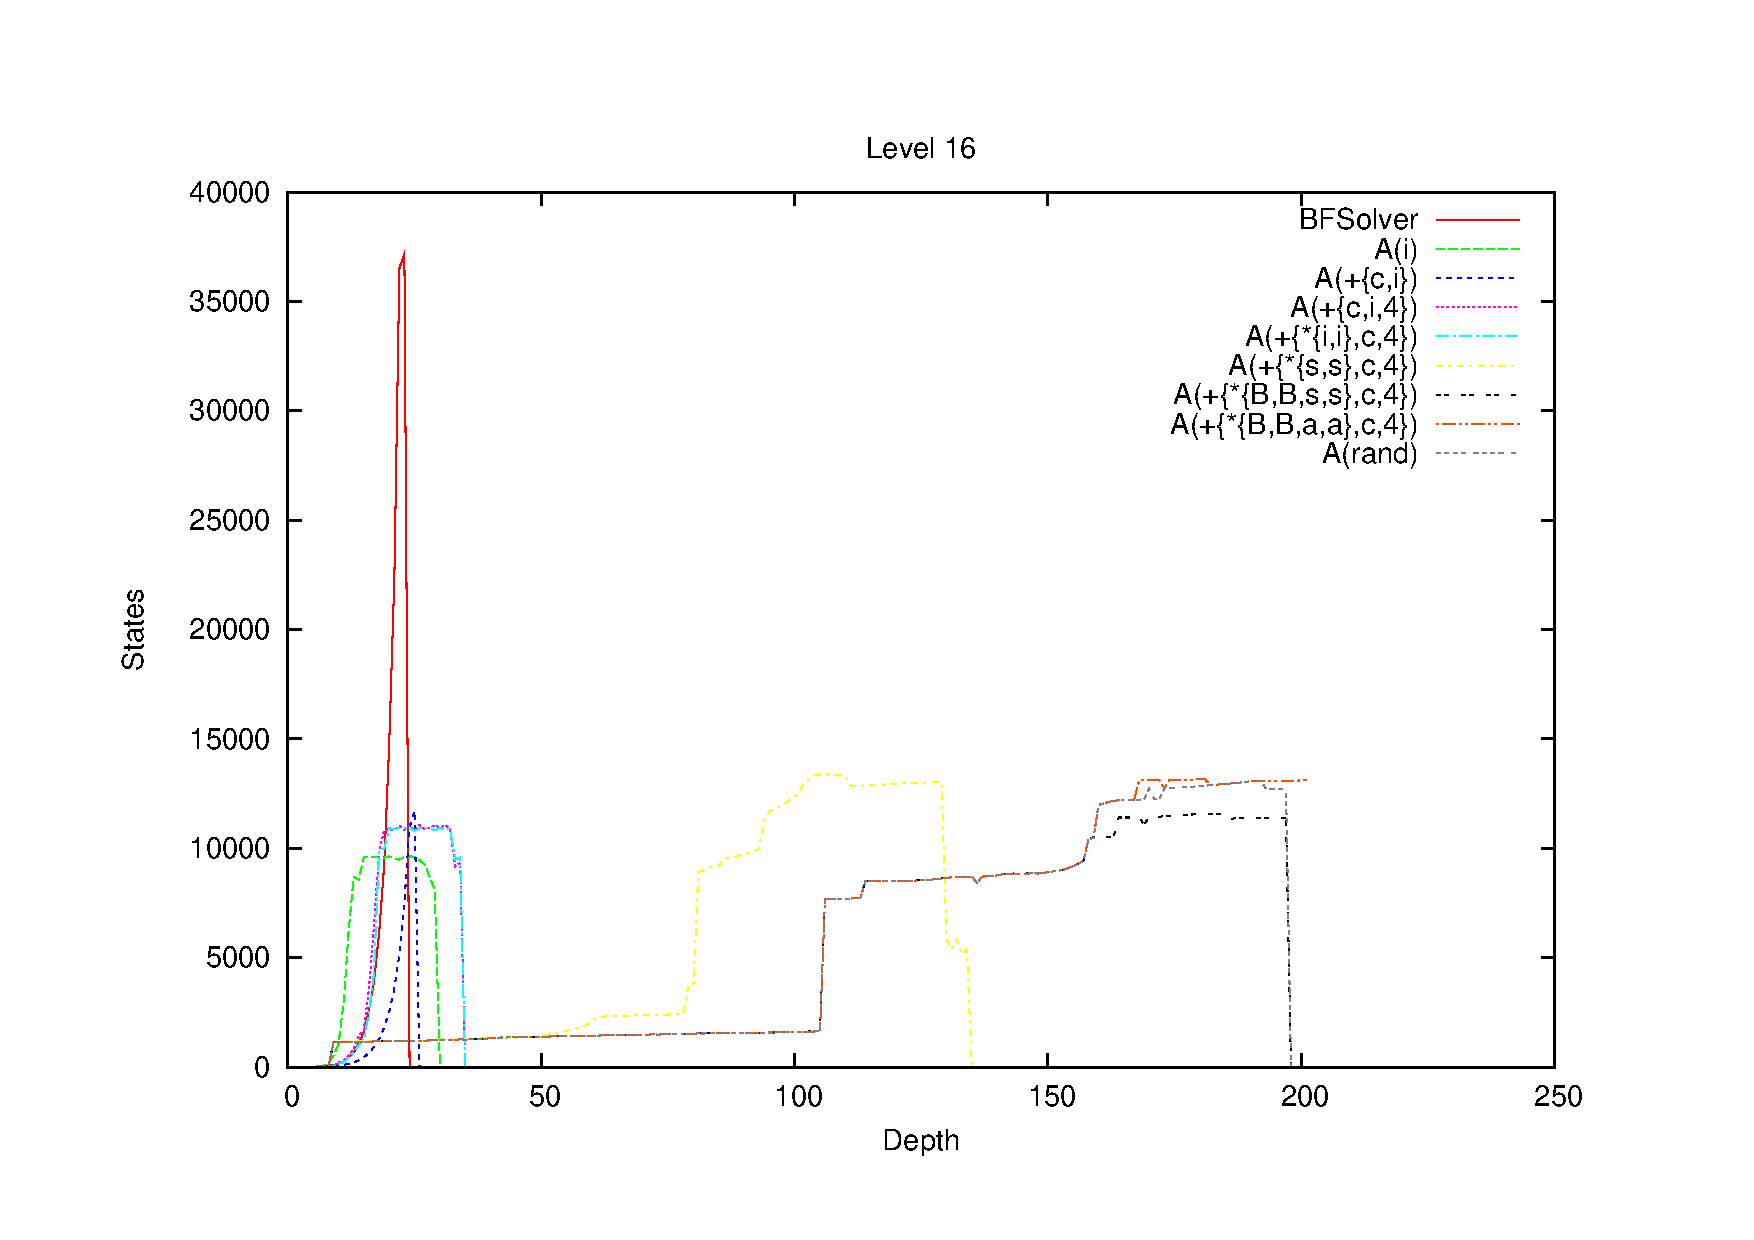
\includegraphics[width=0.85\textwidth]{level16-5}
  \caption{Level 16}
  \label{fig:level16-stats}
\end{figure}
 
\begin{figure}
  \centering
  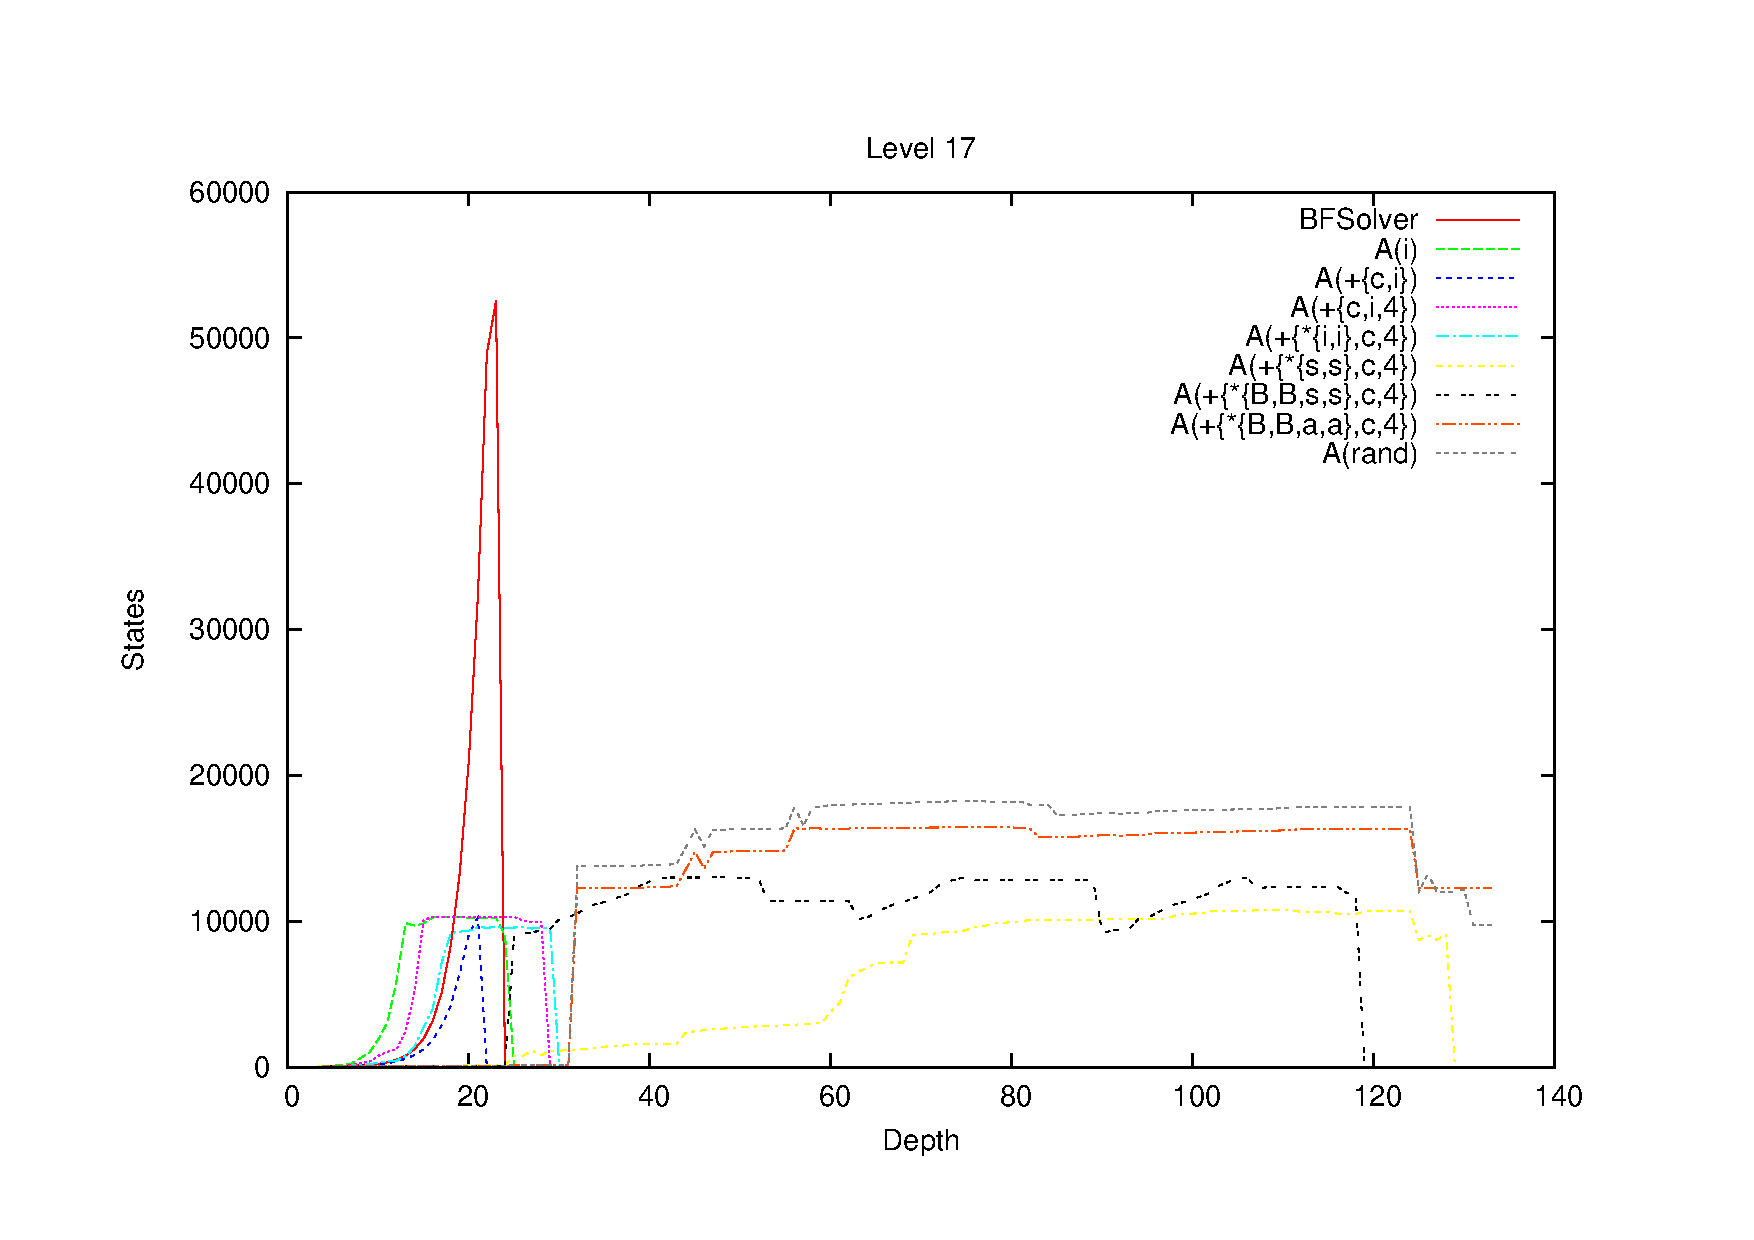
\includegraphics[width=0.85\textwidth]{level17-5}
  \caption{Level 17}
  \label{fig:level17-stats}
\end{figure}

\begin{figure}
  \centering
  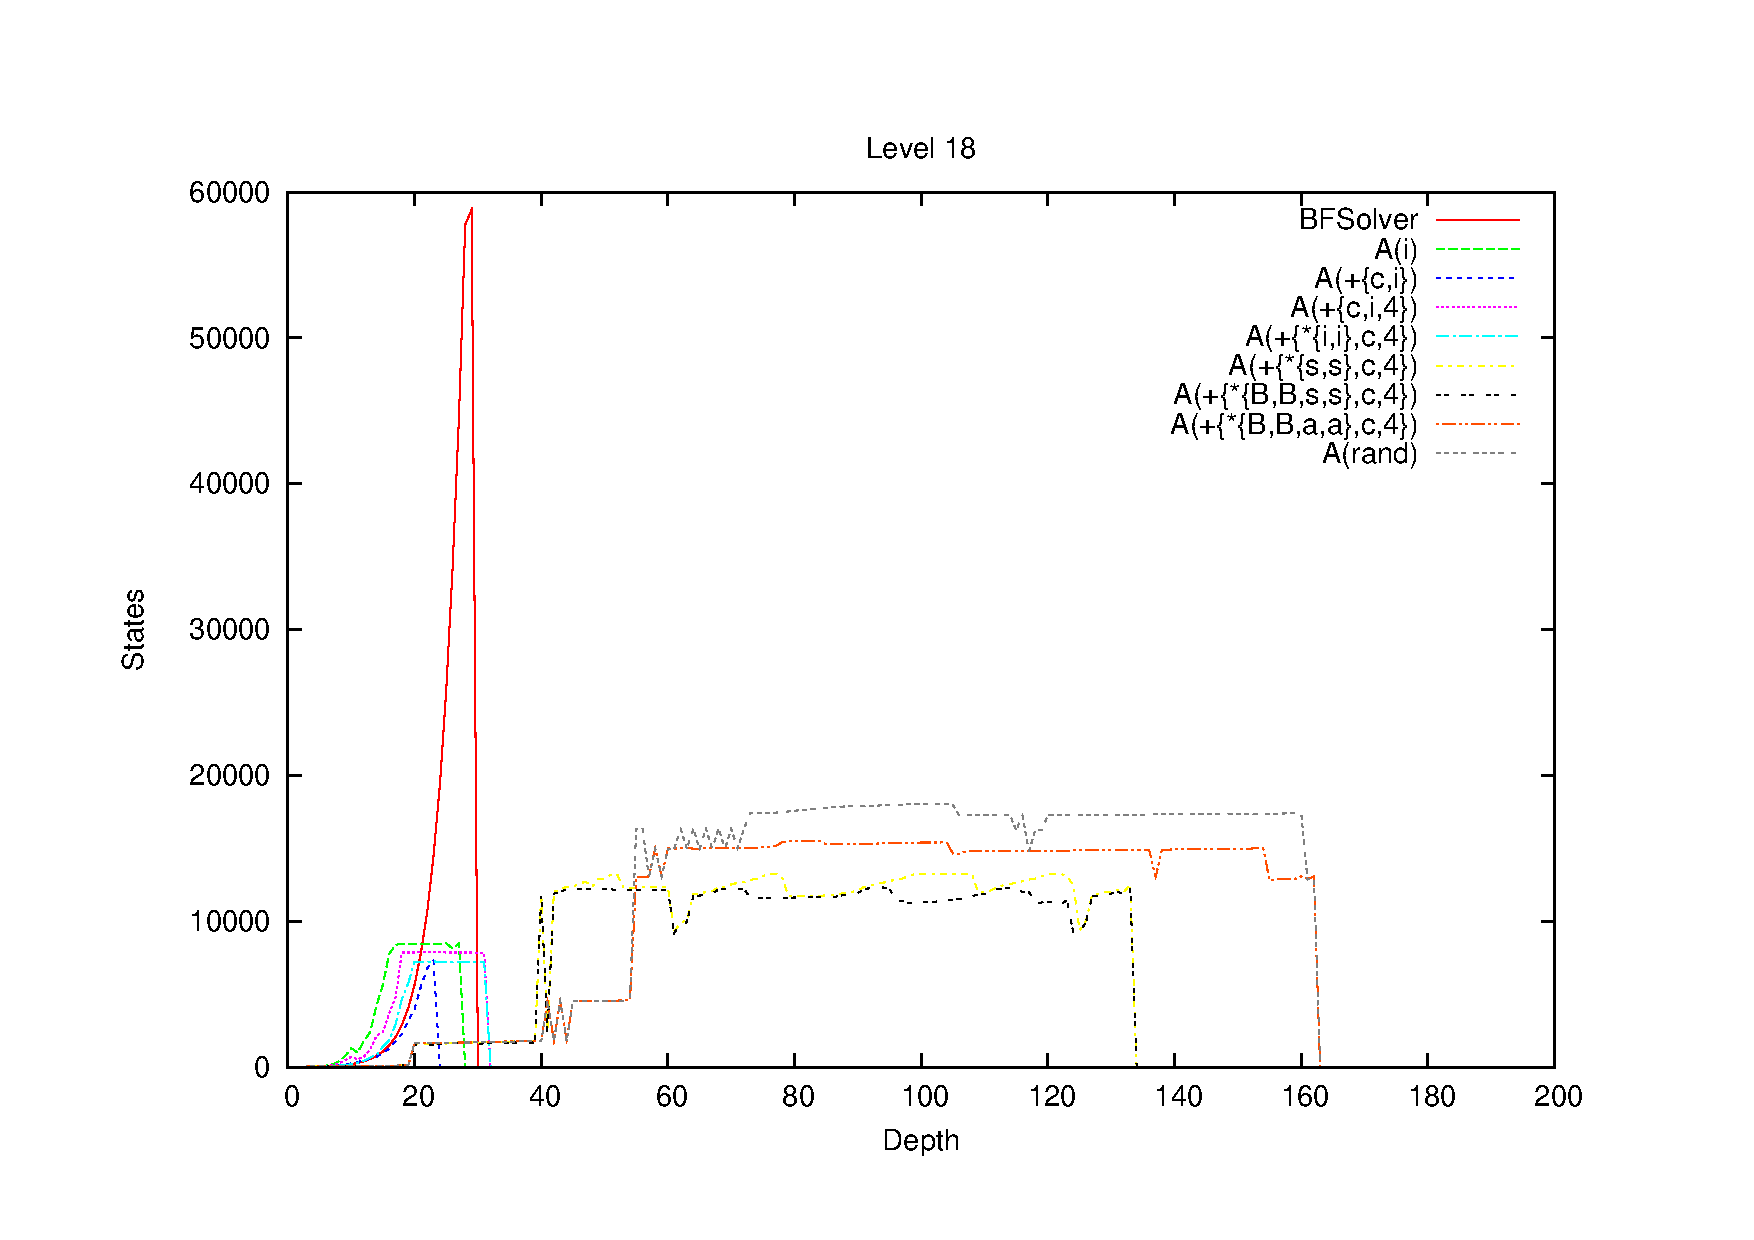
\includegraphics[width=0.85\textwidth]{level18-5}
  \caption{Level 18}
  \label{fig:level18-stats}
\end{figure}
 
\begin{figure}
  \centering
  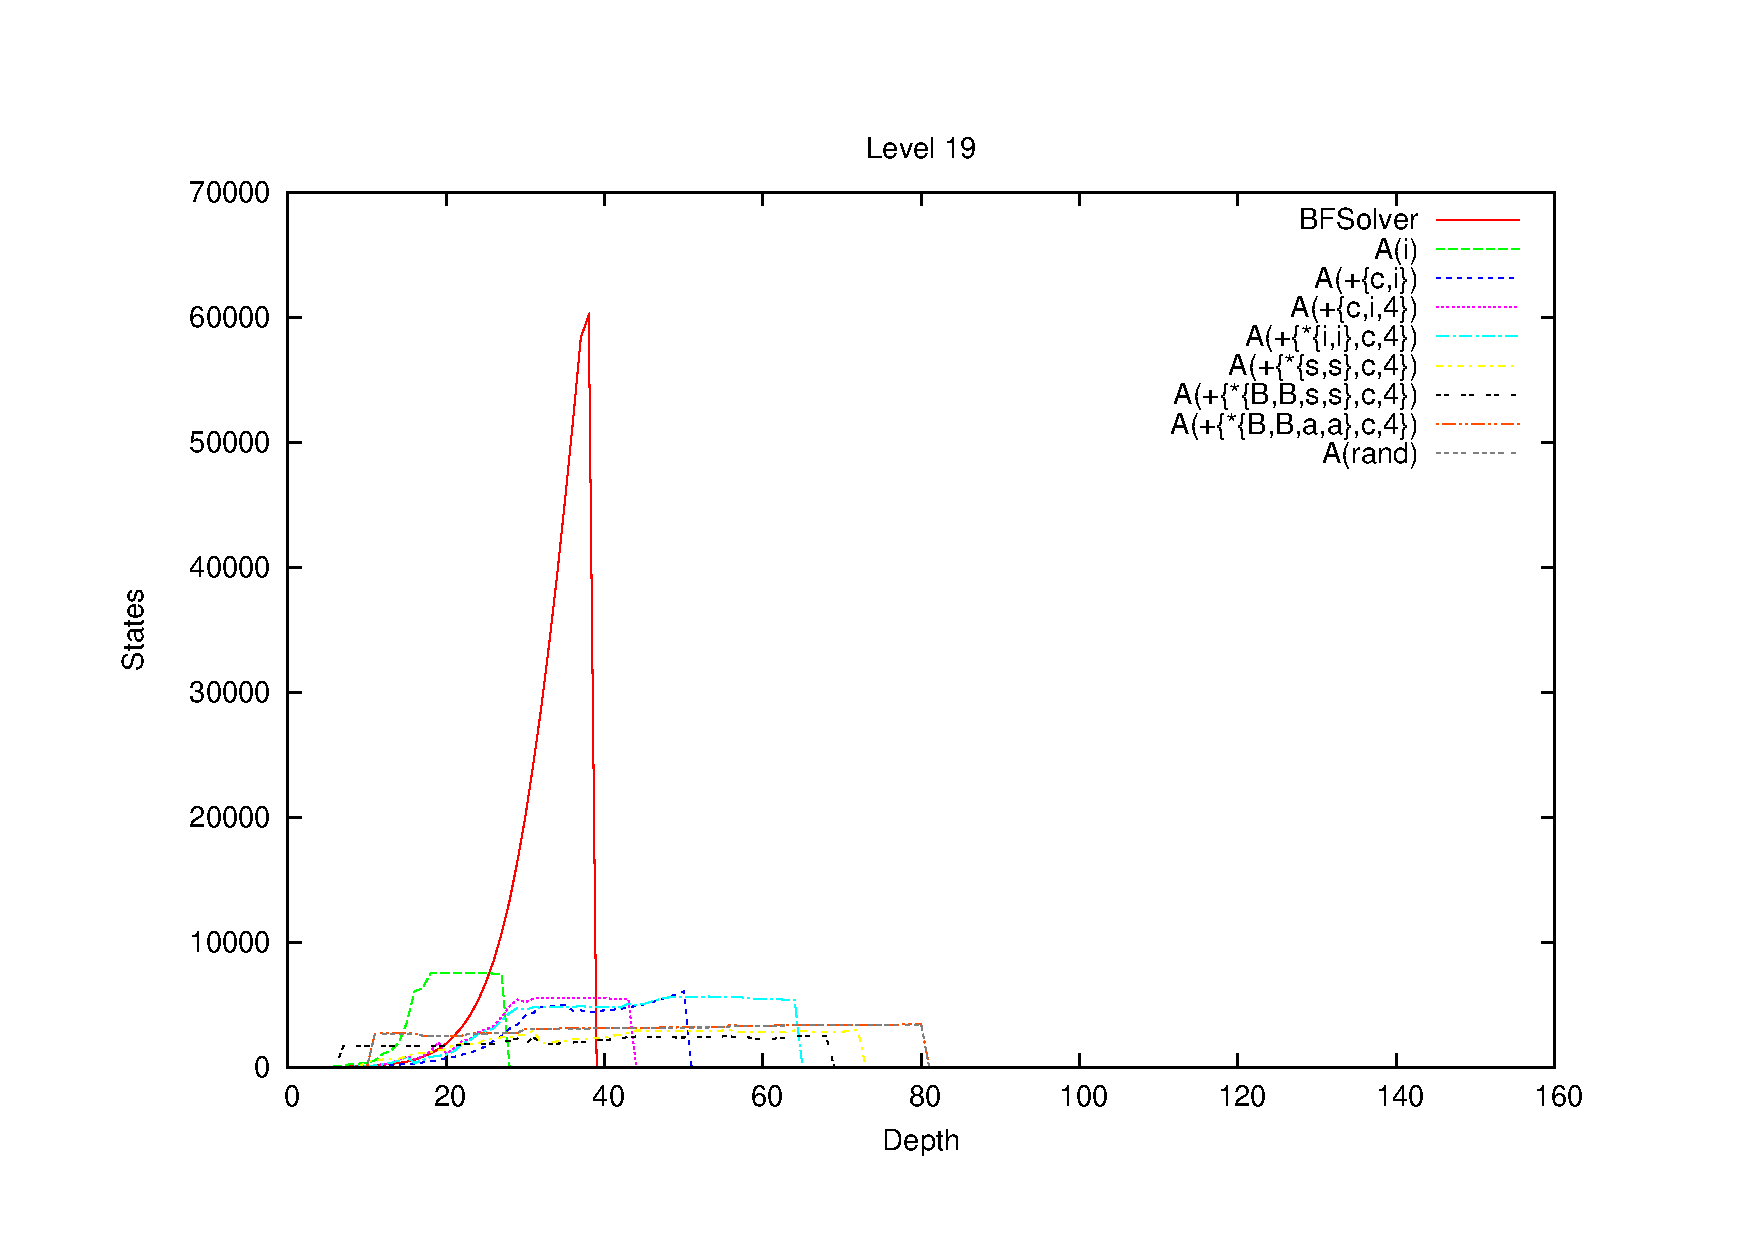
\includegraphics[width=0.85\textwidth]{level19-5}
  \caption{Level 19}
  \label{fig:level19-stats}
\end{figure}

\begin{figure}
  \centering
  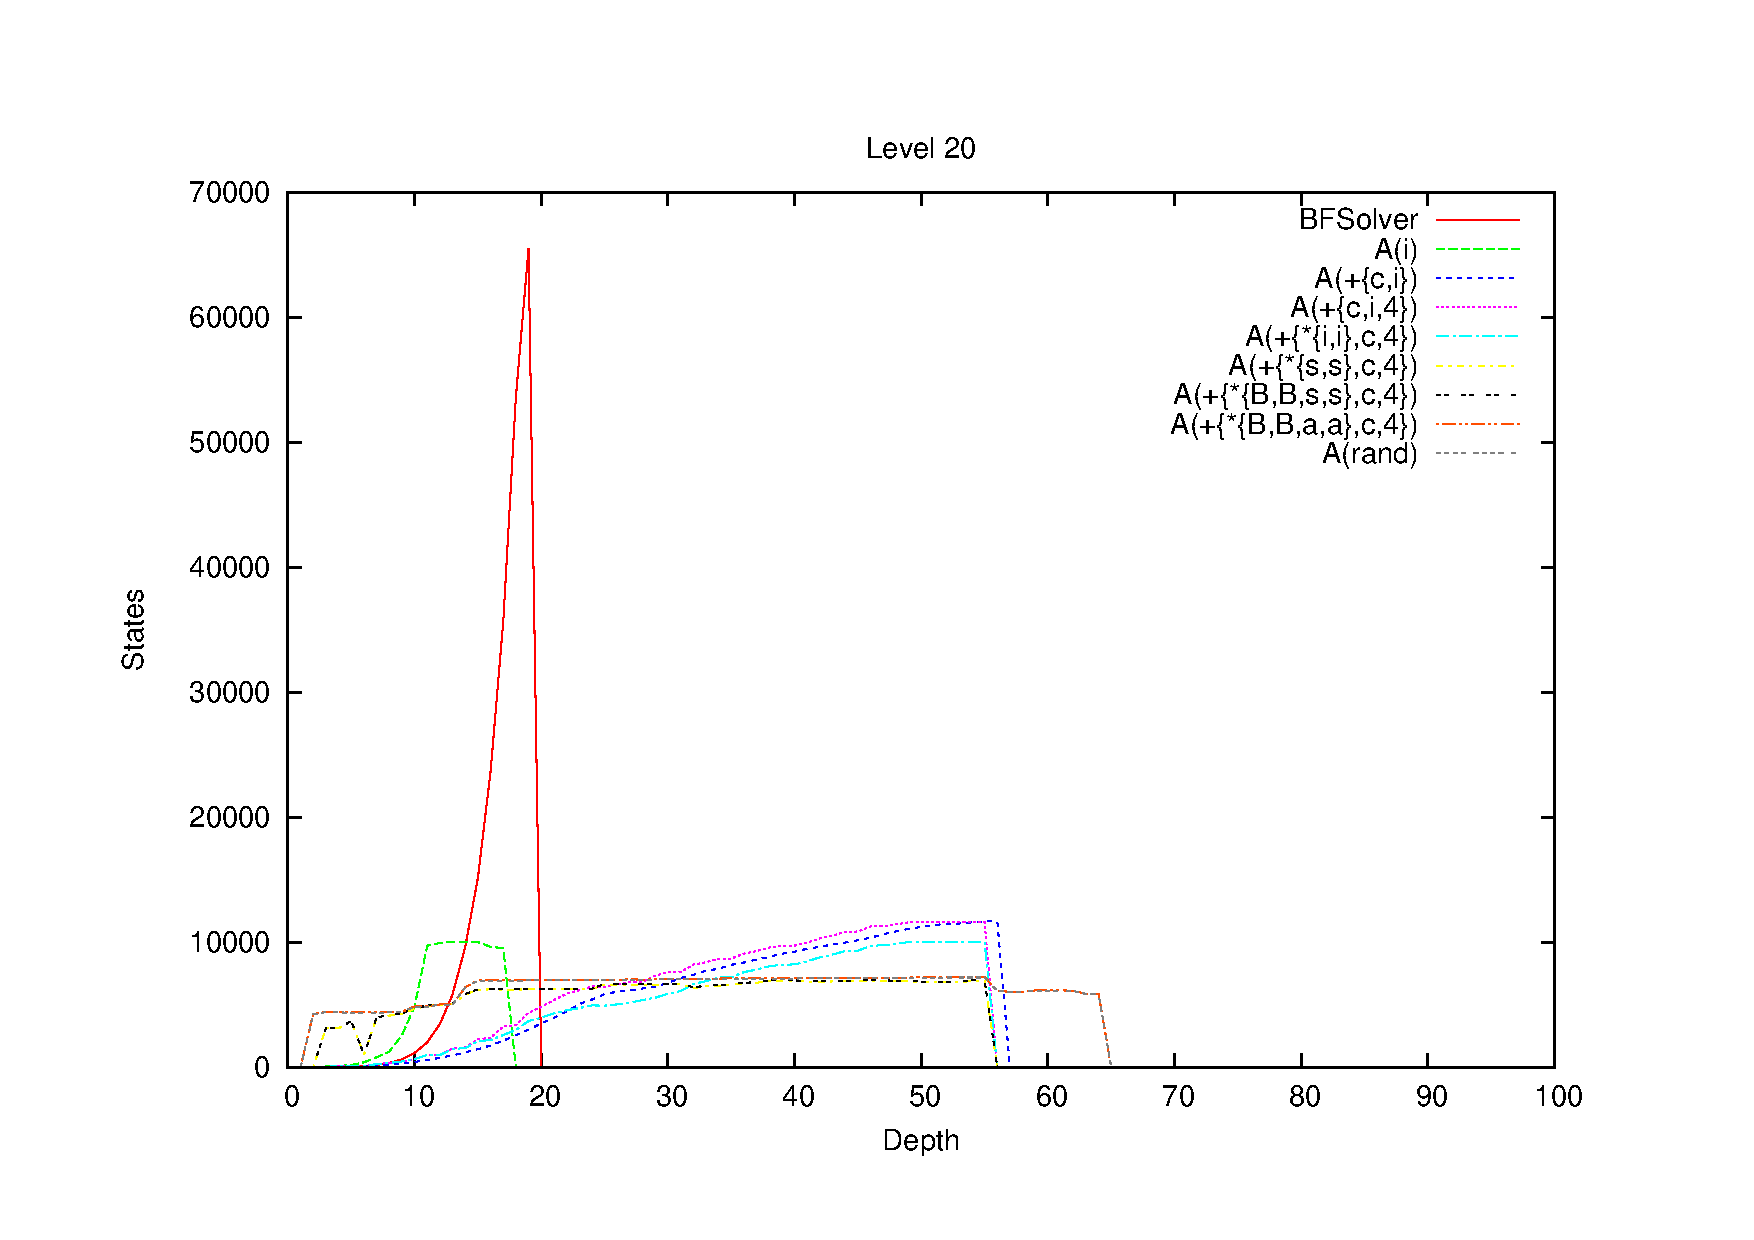
\includegraphics[width=0.85\textwidth]{level20-5}
  \caption{Level 20}
  \label{fig:level20-stats}
\end{figure}

\clearpage
 
\begin{figure}
  \centering
  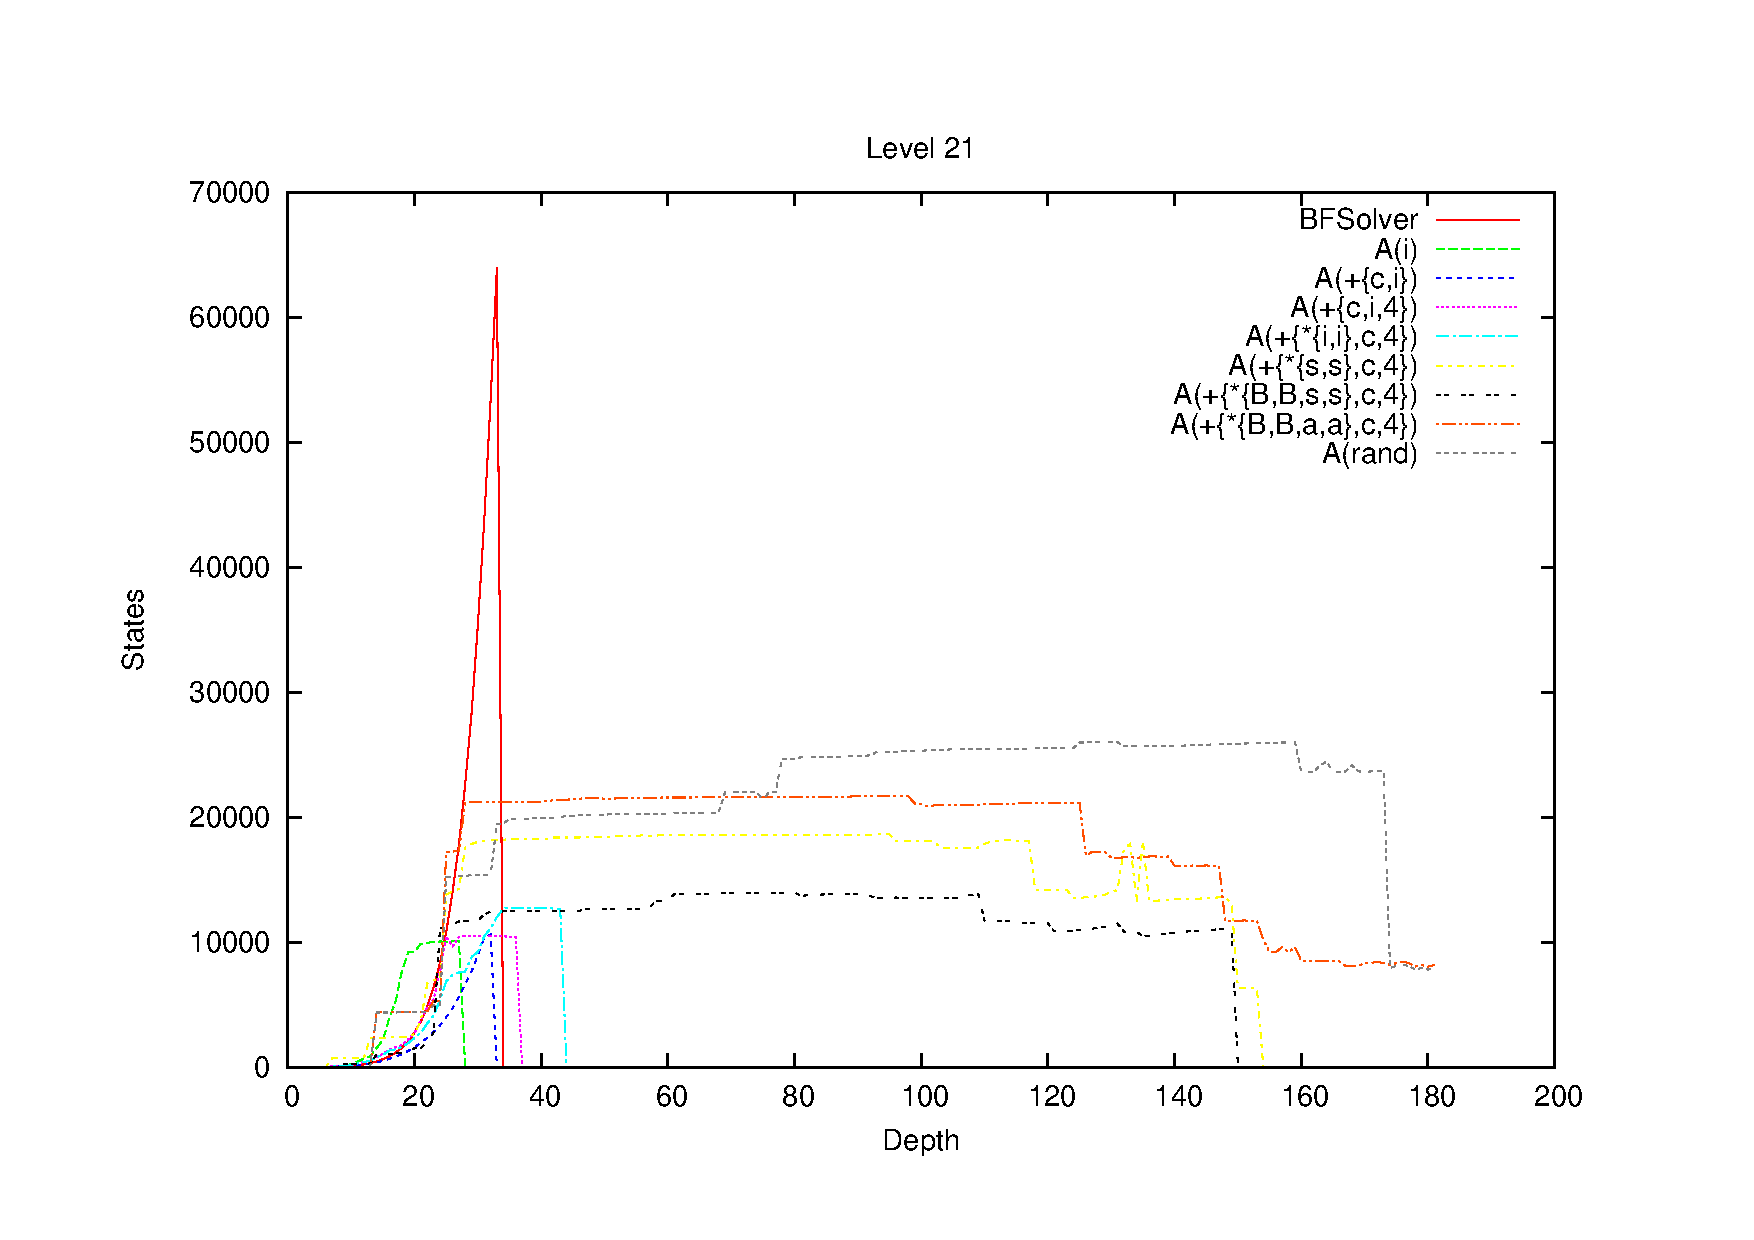
\includegraphics[width=0.85\textwidth]{level21-5}
  \caption{Level 21}
  \label{fig:level21-stats}
\end{figure}

\begin{figure}
  \centering
  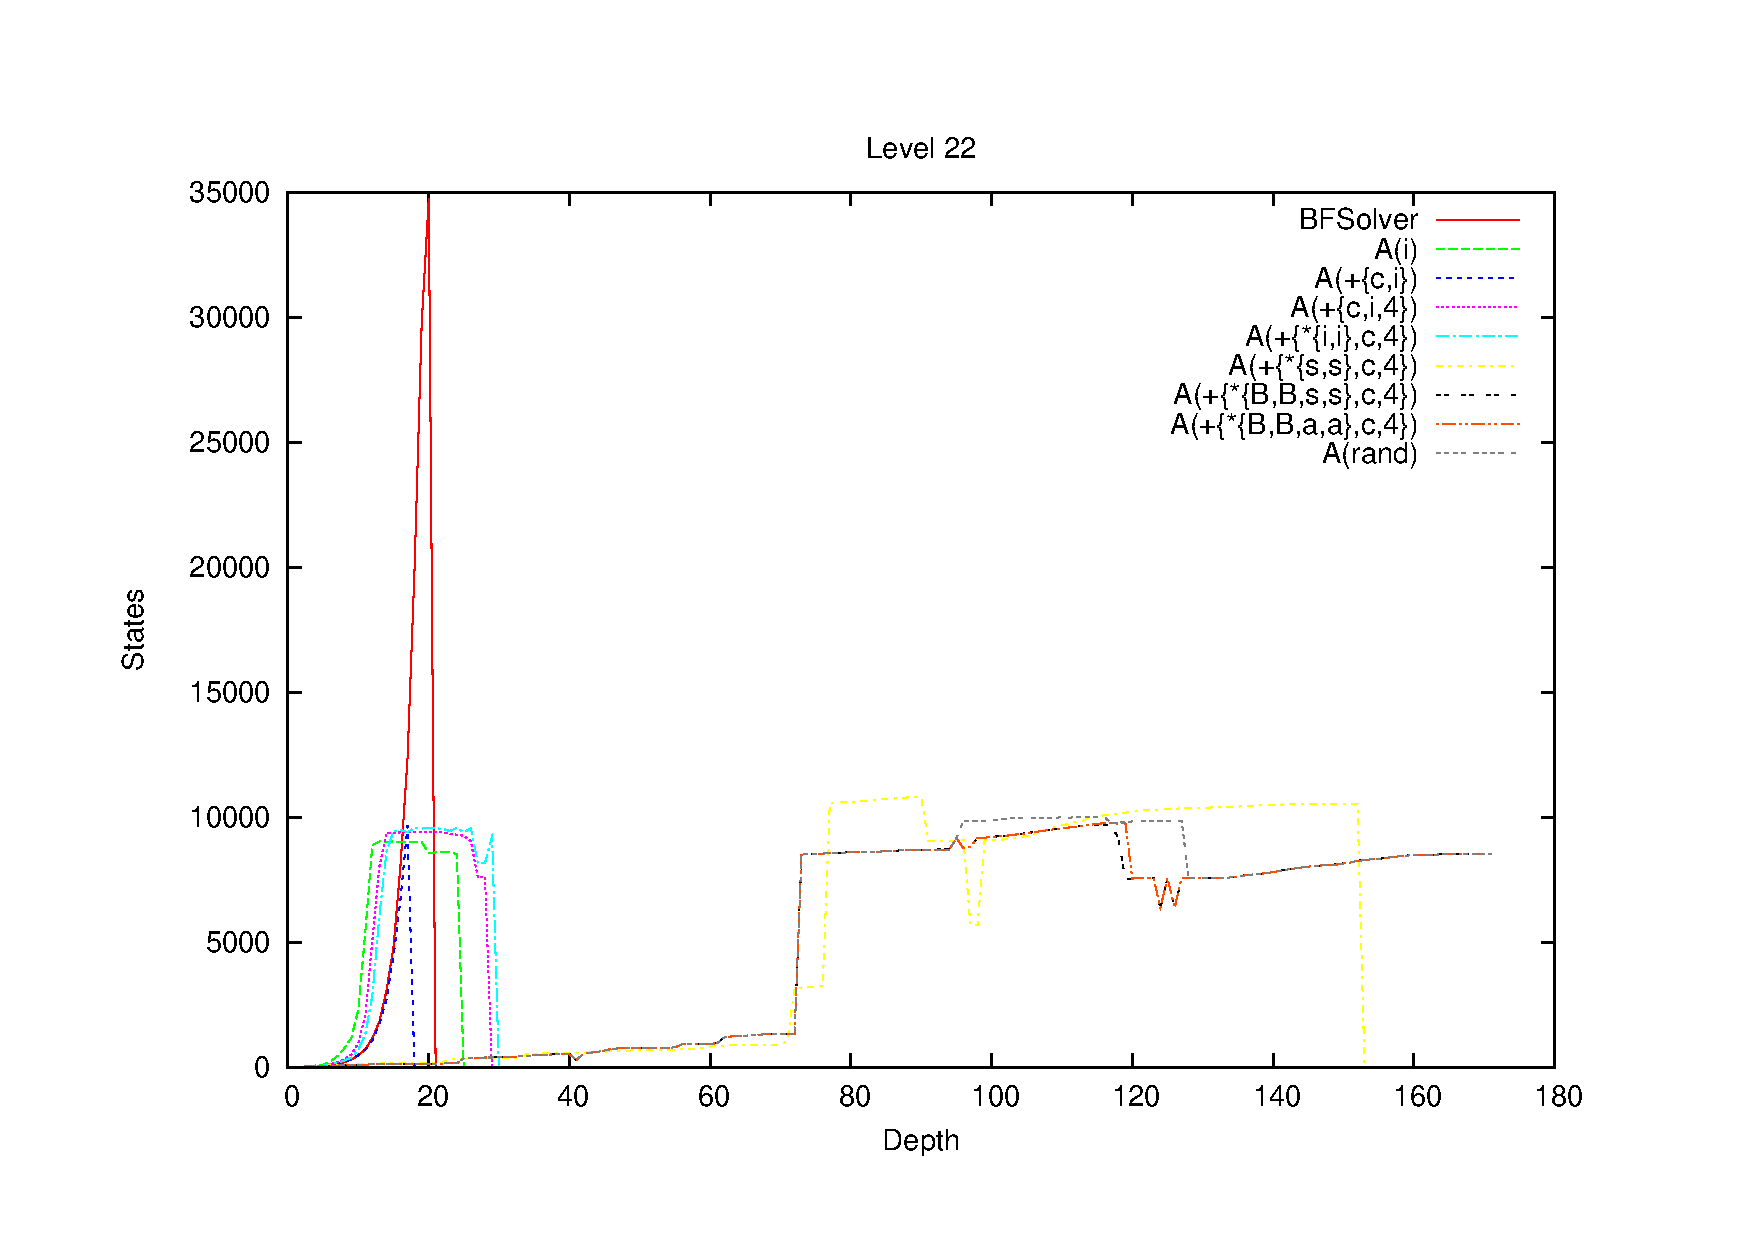
\includegraphics[width=0.85\textwidth]{level22-5}
  \caption{Level 22}
  \label{fig:level2-stats}
\end{figure}
 
\begin{figure}
  \centering
  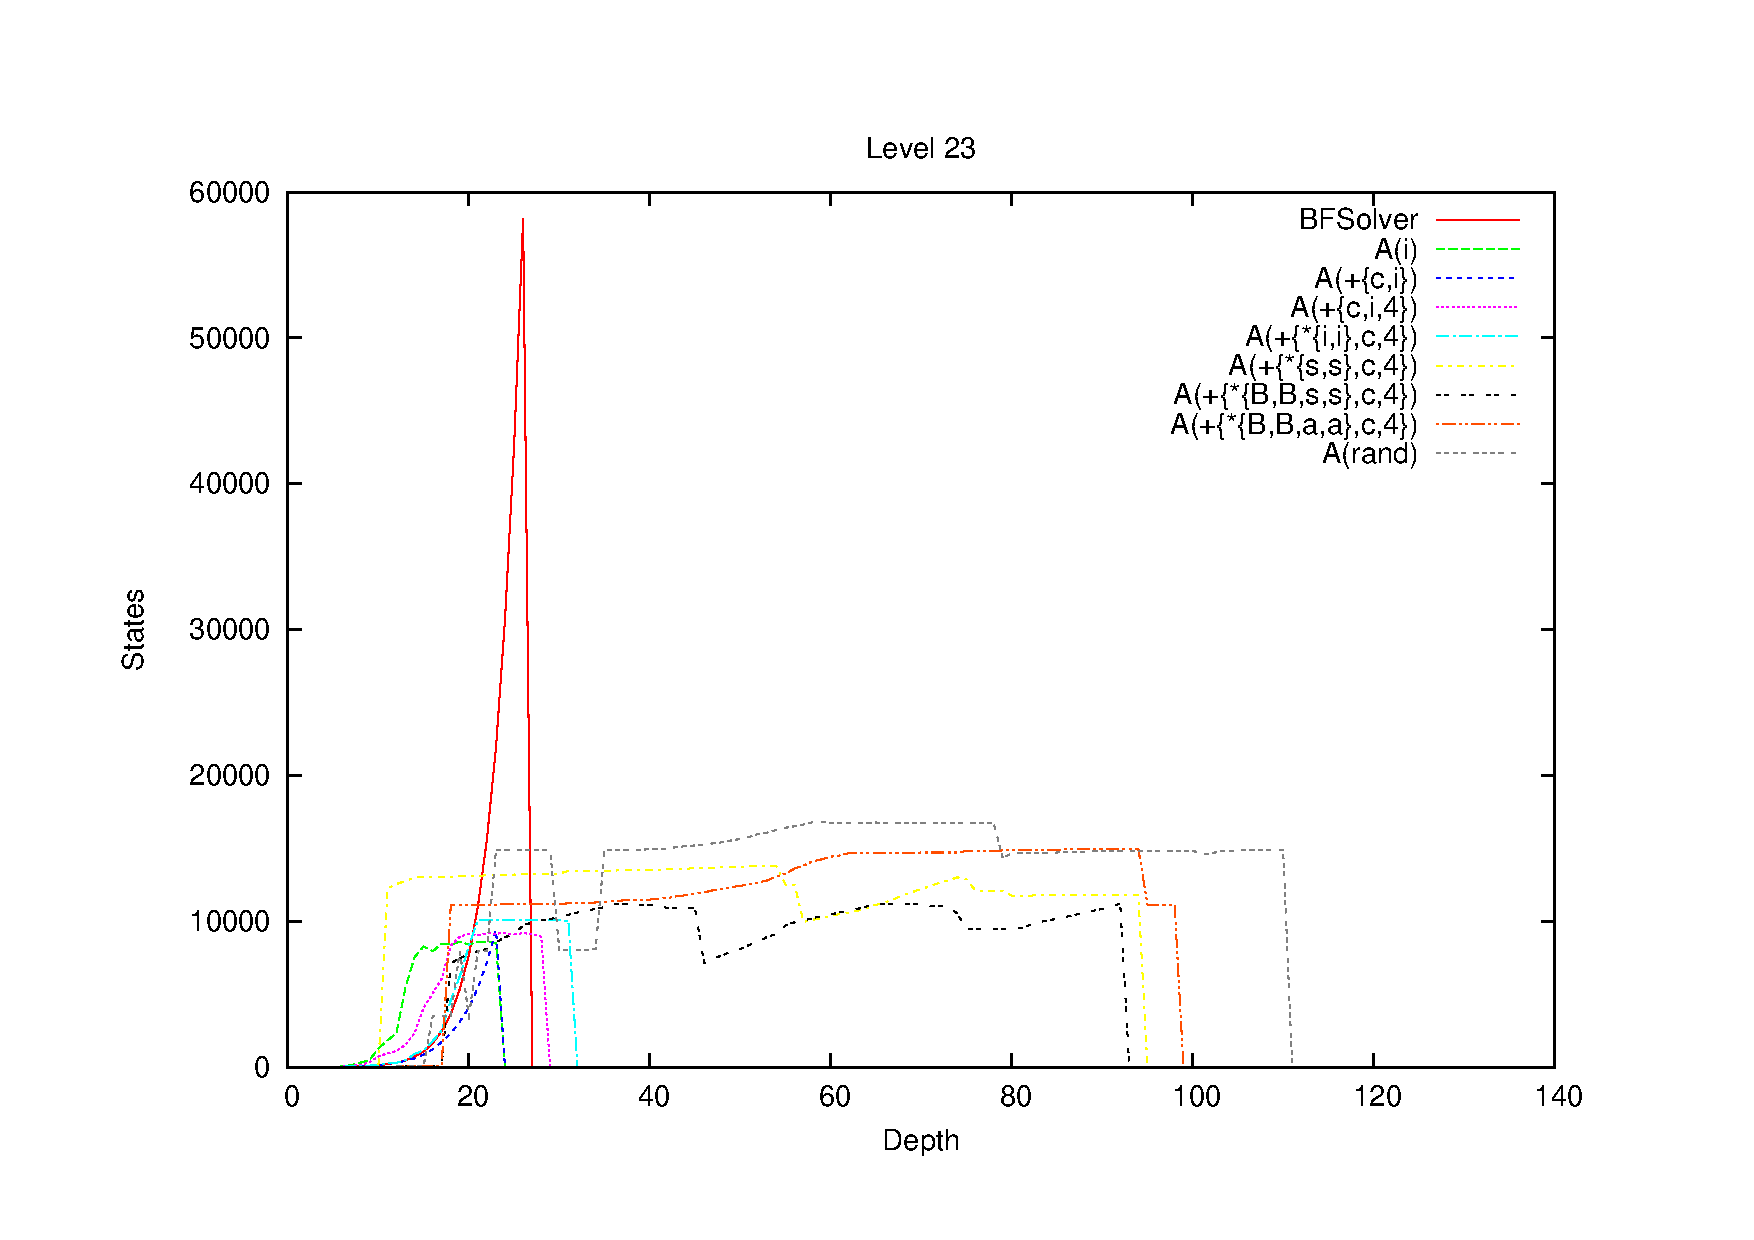
\includegraphics[width=0.85\textwidth]{level23-5}
  \caption{Level 23}
  \label{fig:level23-stats}
\end{figure}

\begin{figure}
  \centering
  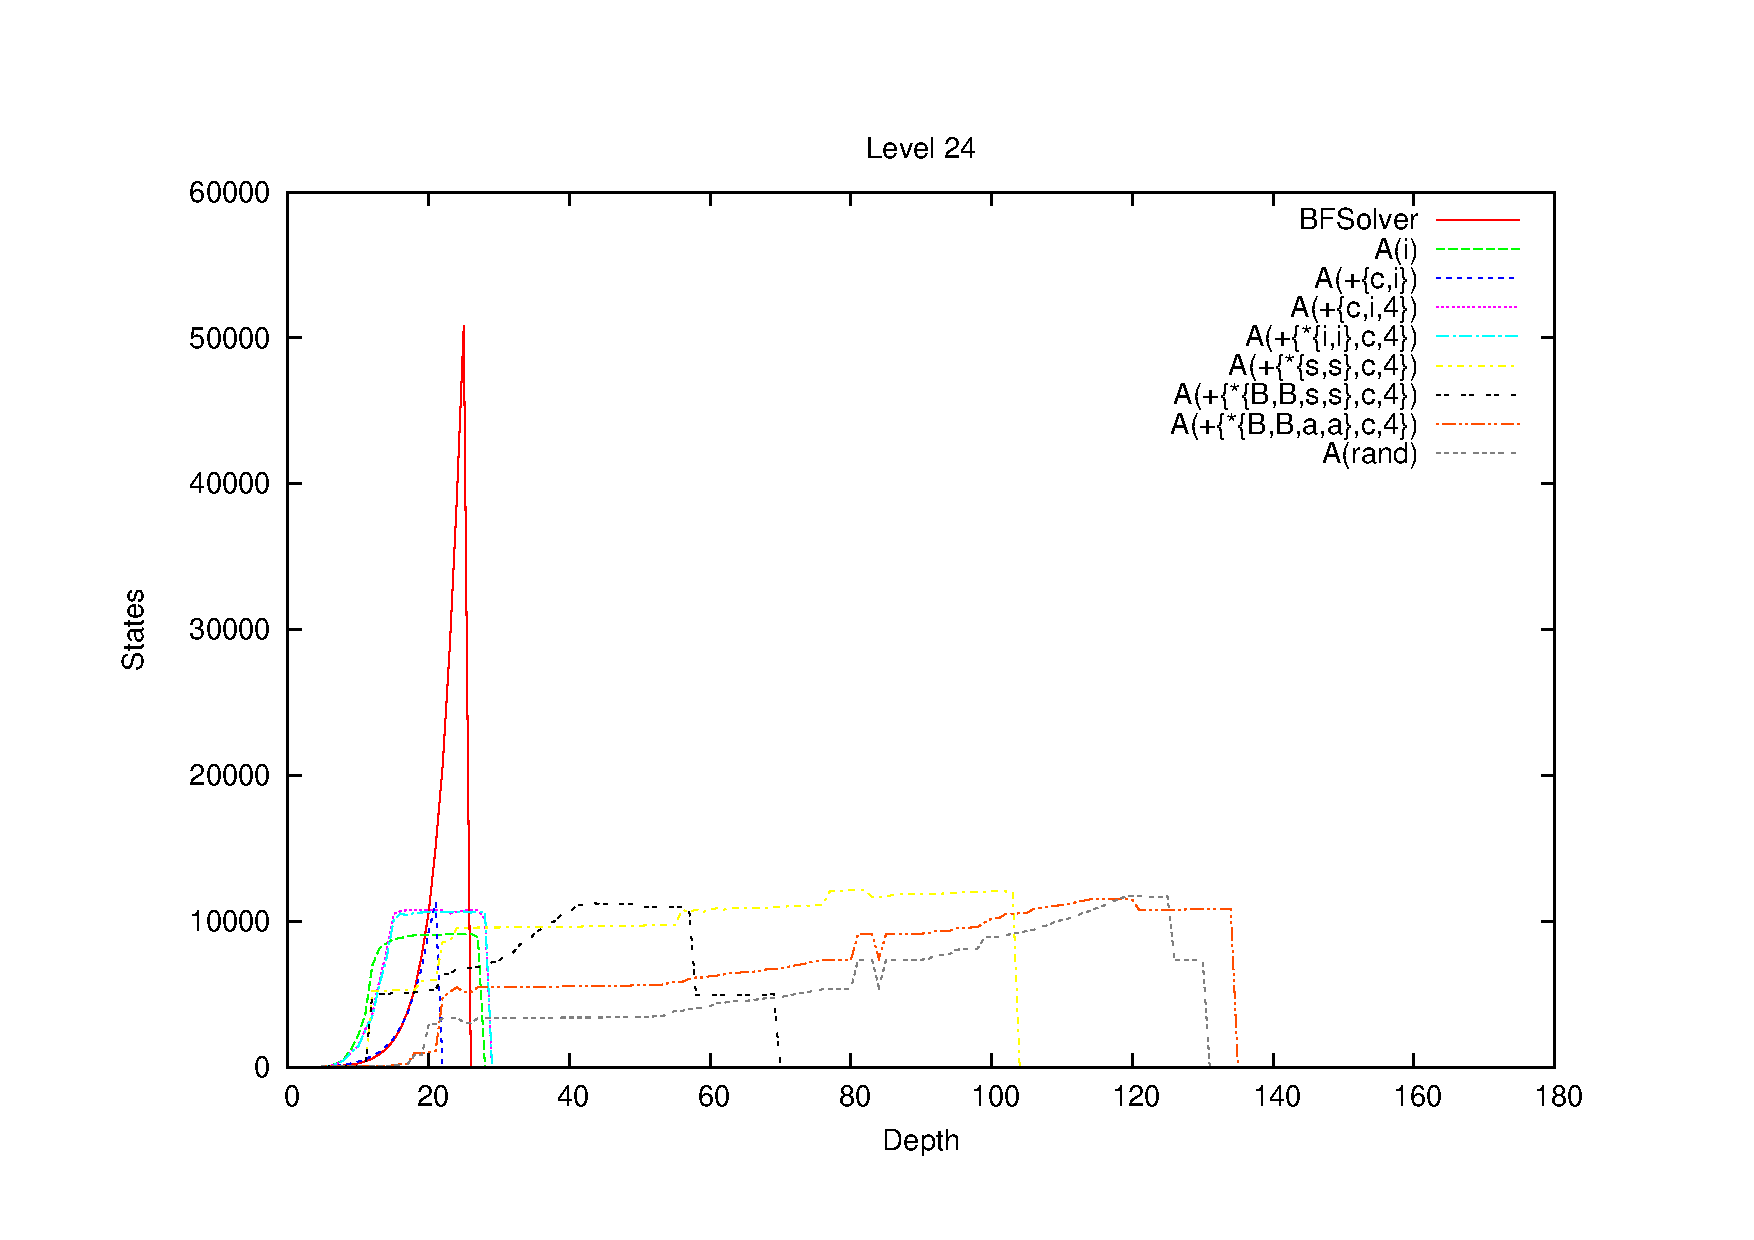
\includegraphics[width=0.85\textwidth]{level24-5}
  \caption{Level 24}
  \label{fig:level24-stats}
\end{figure}
 
\begin{figure}
  \centering
  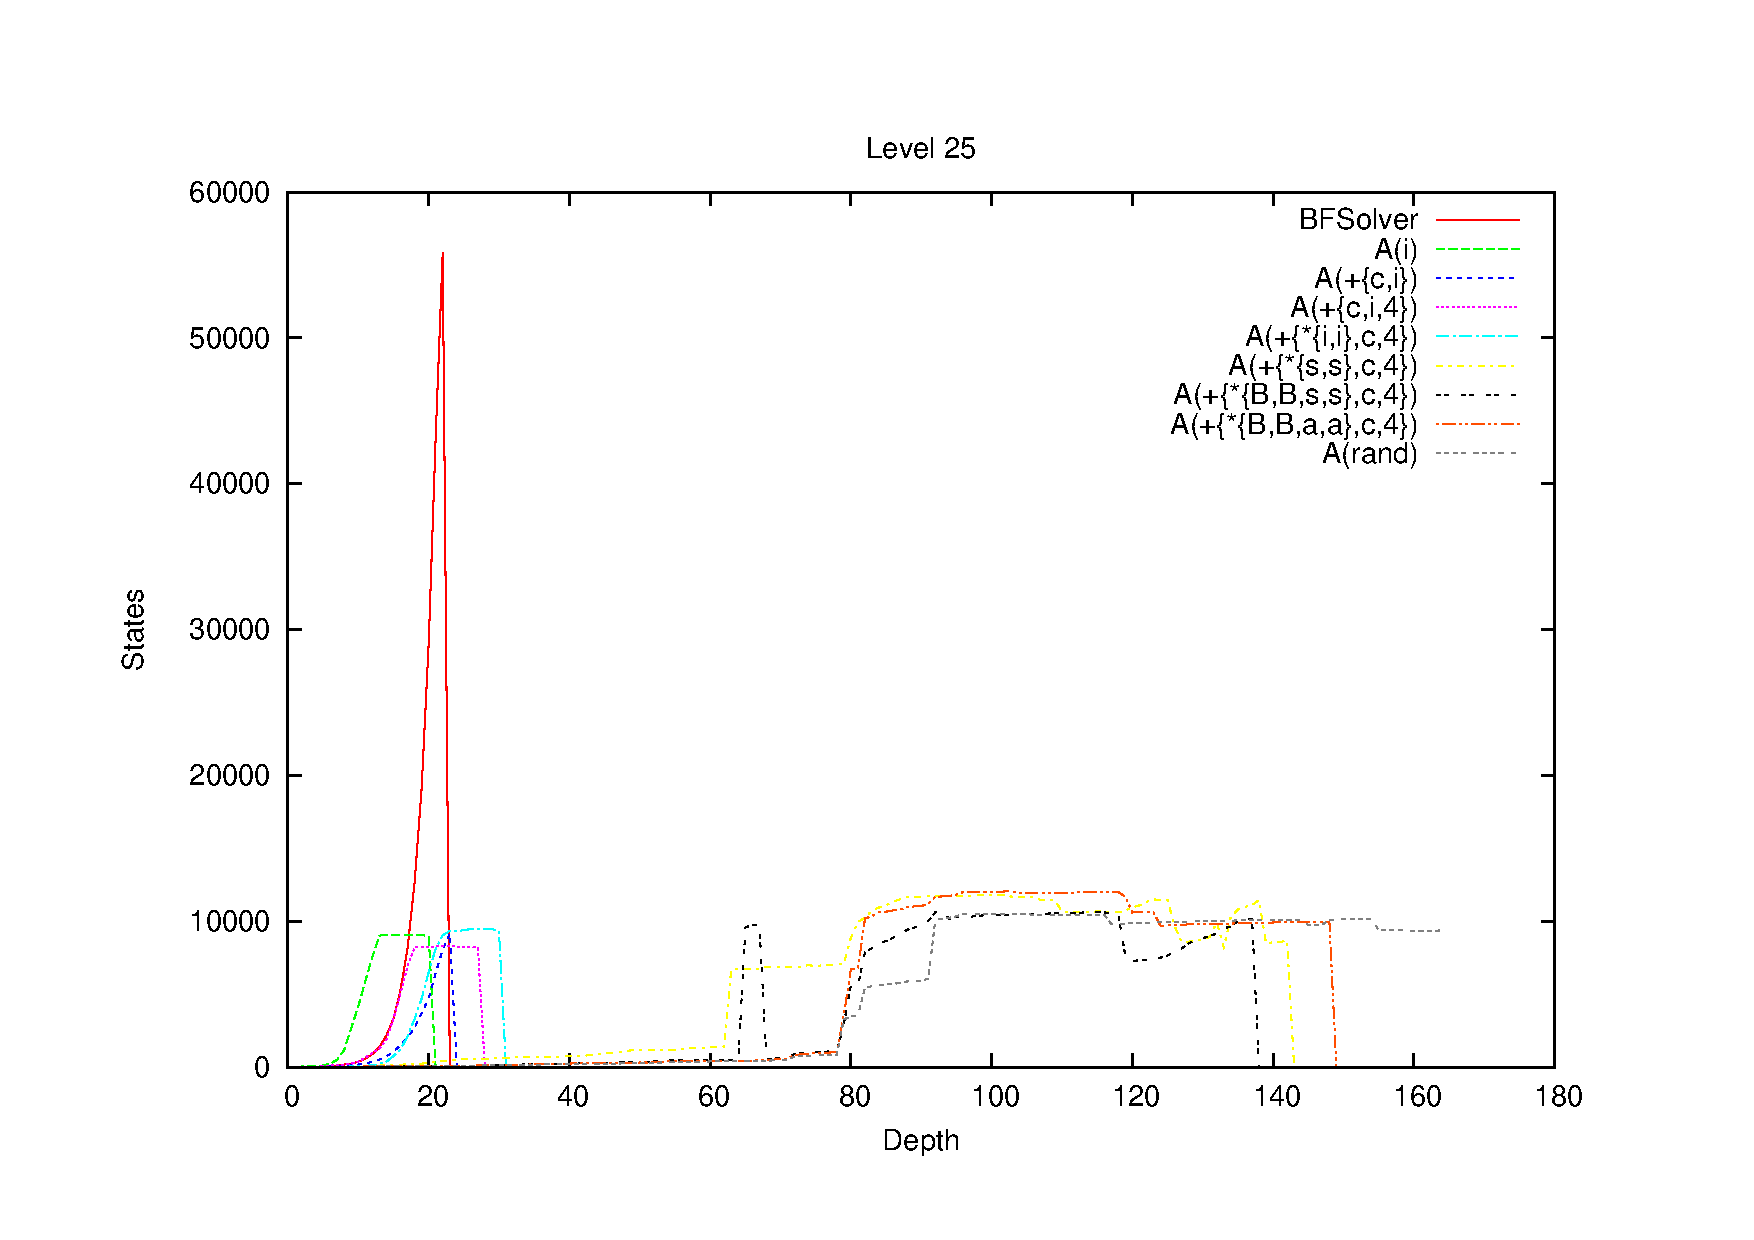
\includegraphics[width=0.85\textwidth]{level25-5}
  \caption{Level 25}
  \label{fig:level25-stats}
\end{figure}

\begin{figure}
  \centering
  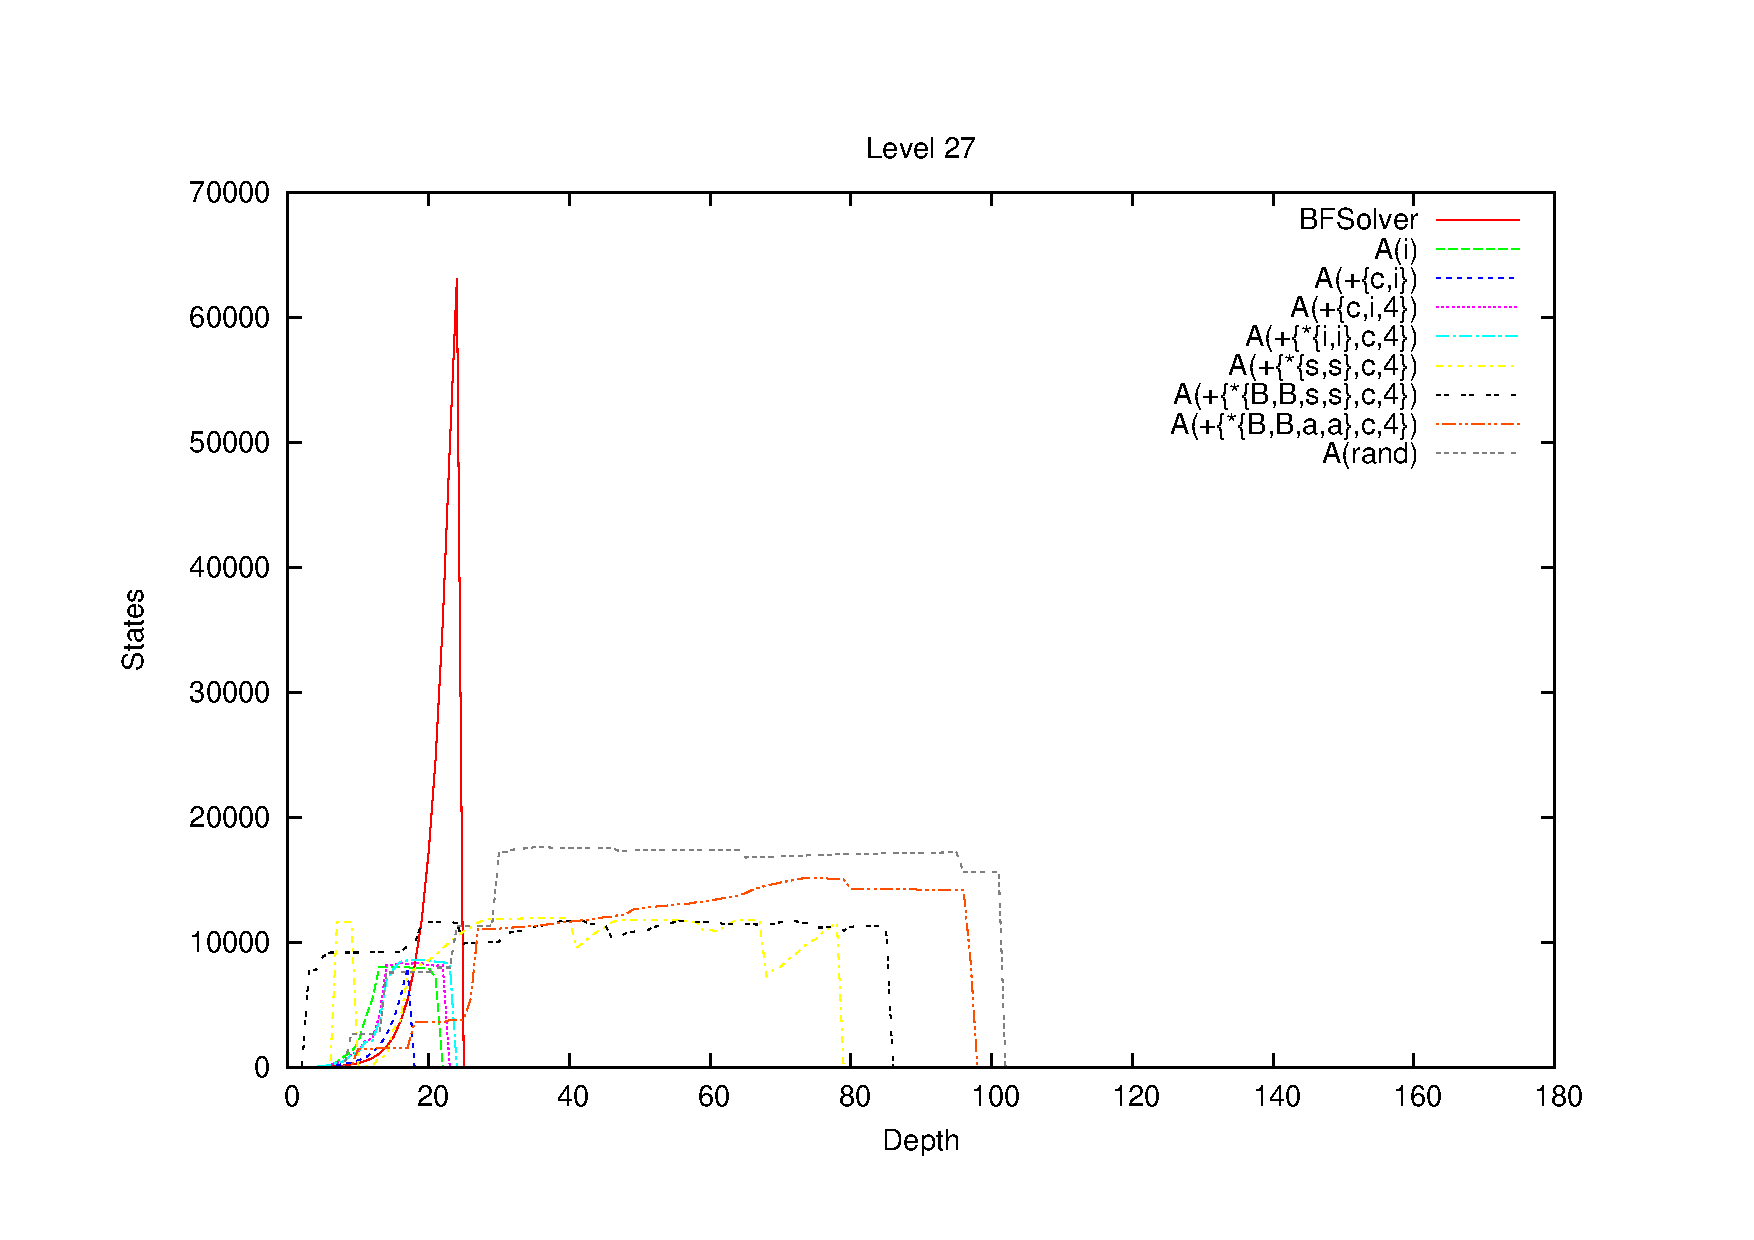
\includegraphics[width=0.85\textwidth]{level27-5}
  \caption{Level 27}
  \label{fig:level27-stats}
\end{figure}
 
\begin{figure}
  \centering
  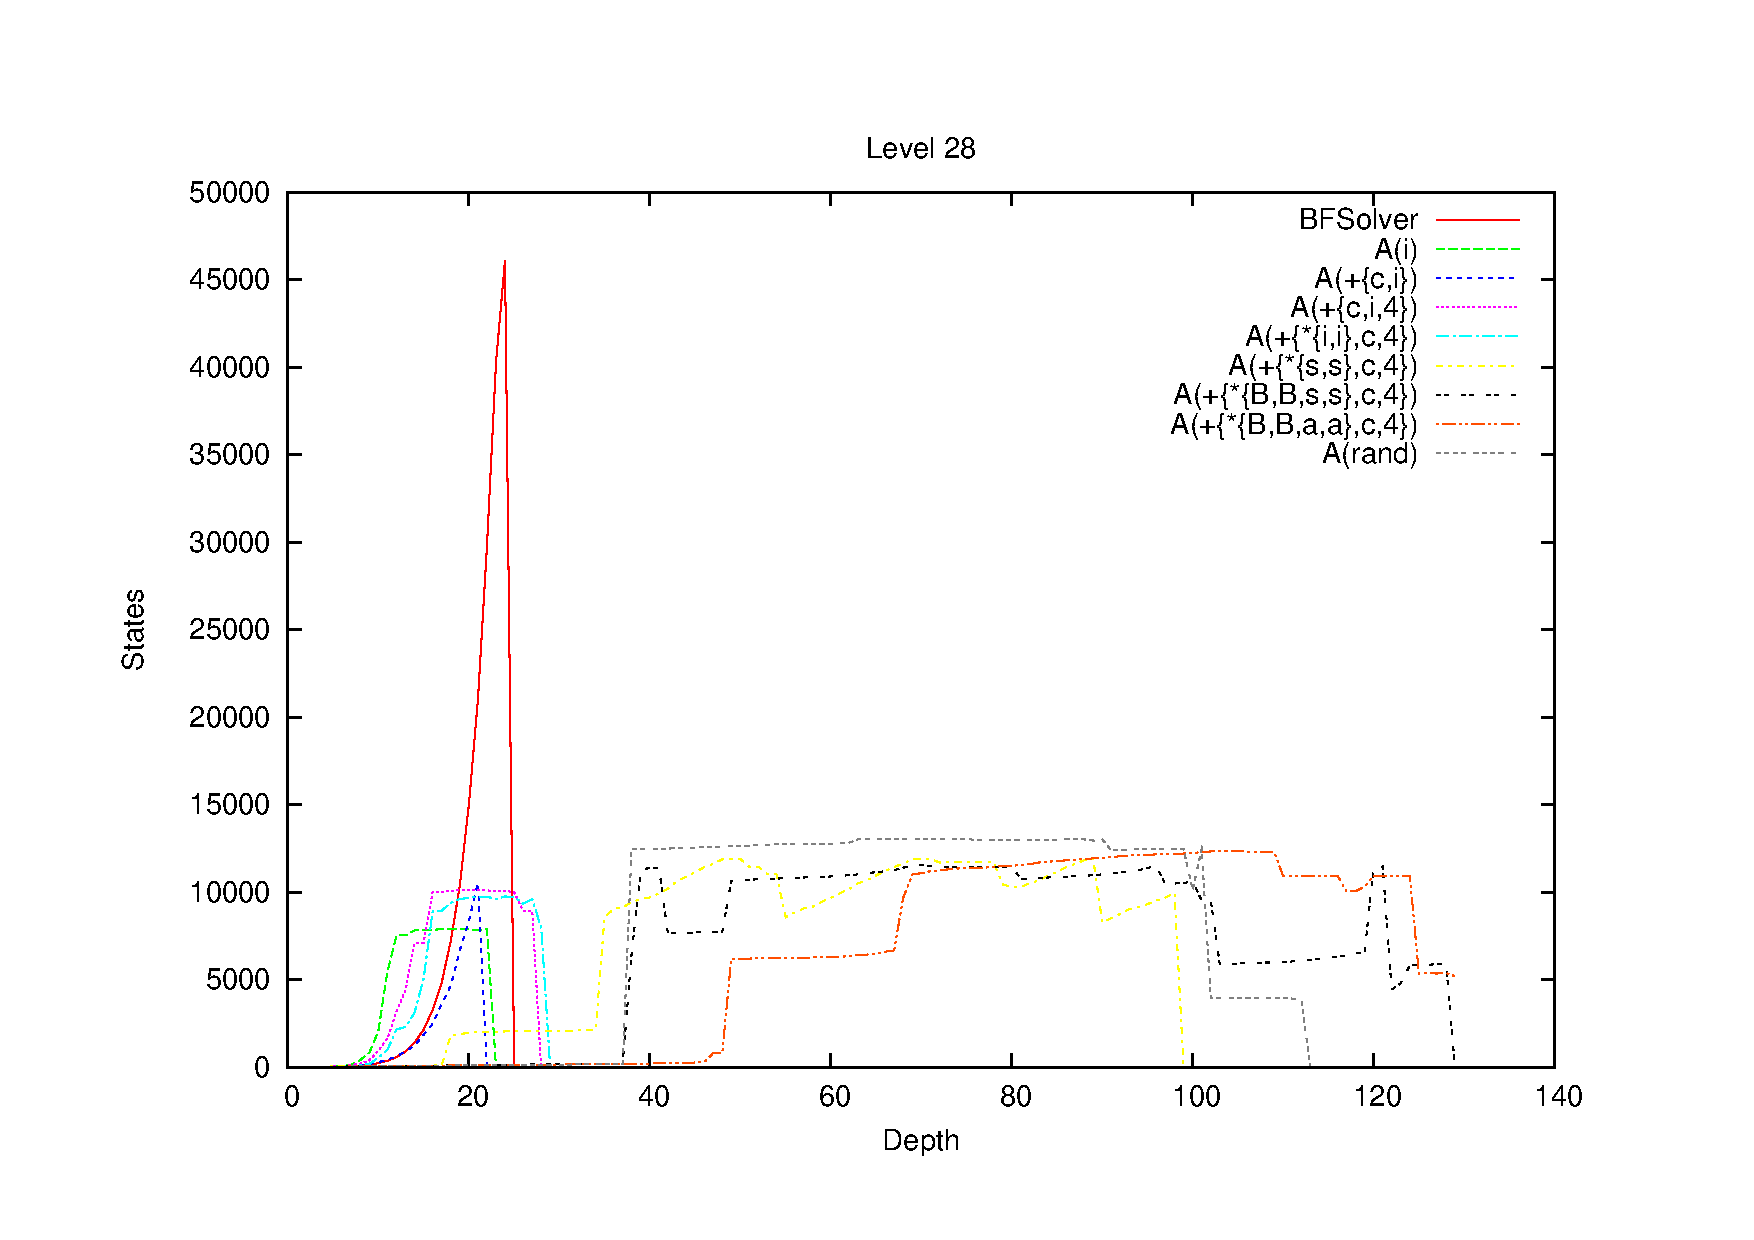
\includegraphics[width=0.85\textwidth]{level28-5}
  \caption{Level 28}
  \label{fig:level28-stats}
\end{figure}

\begin{figure}
  \centering
  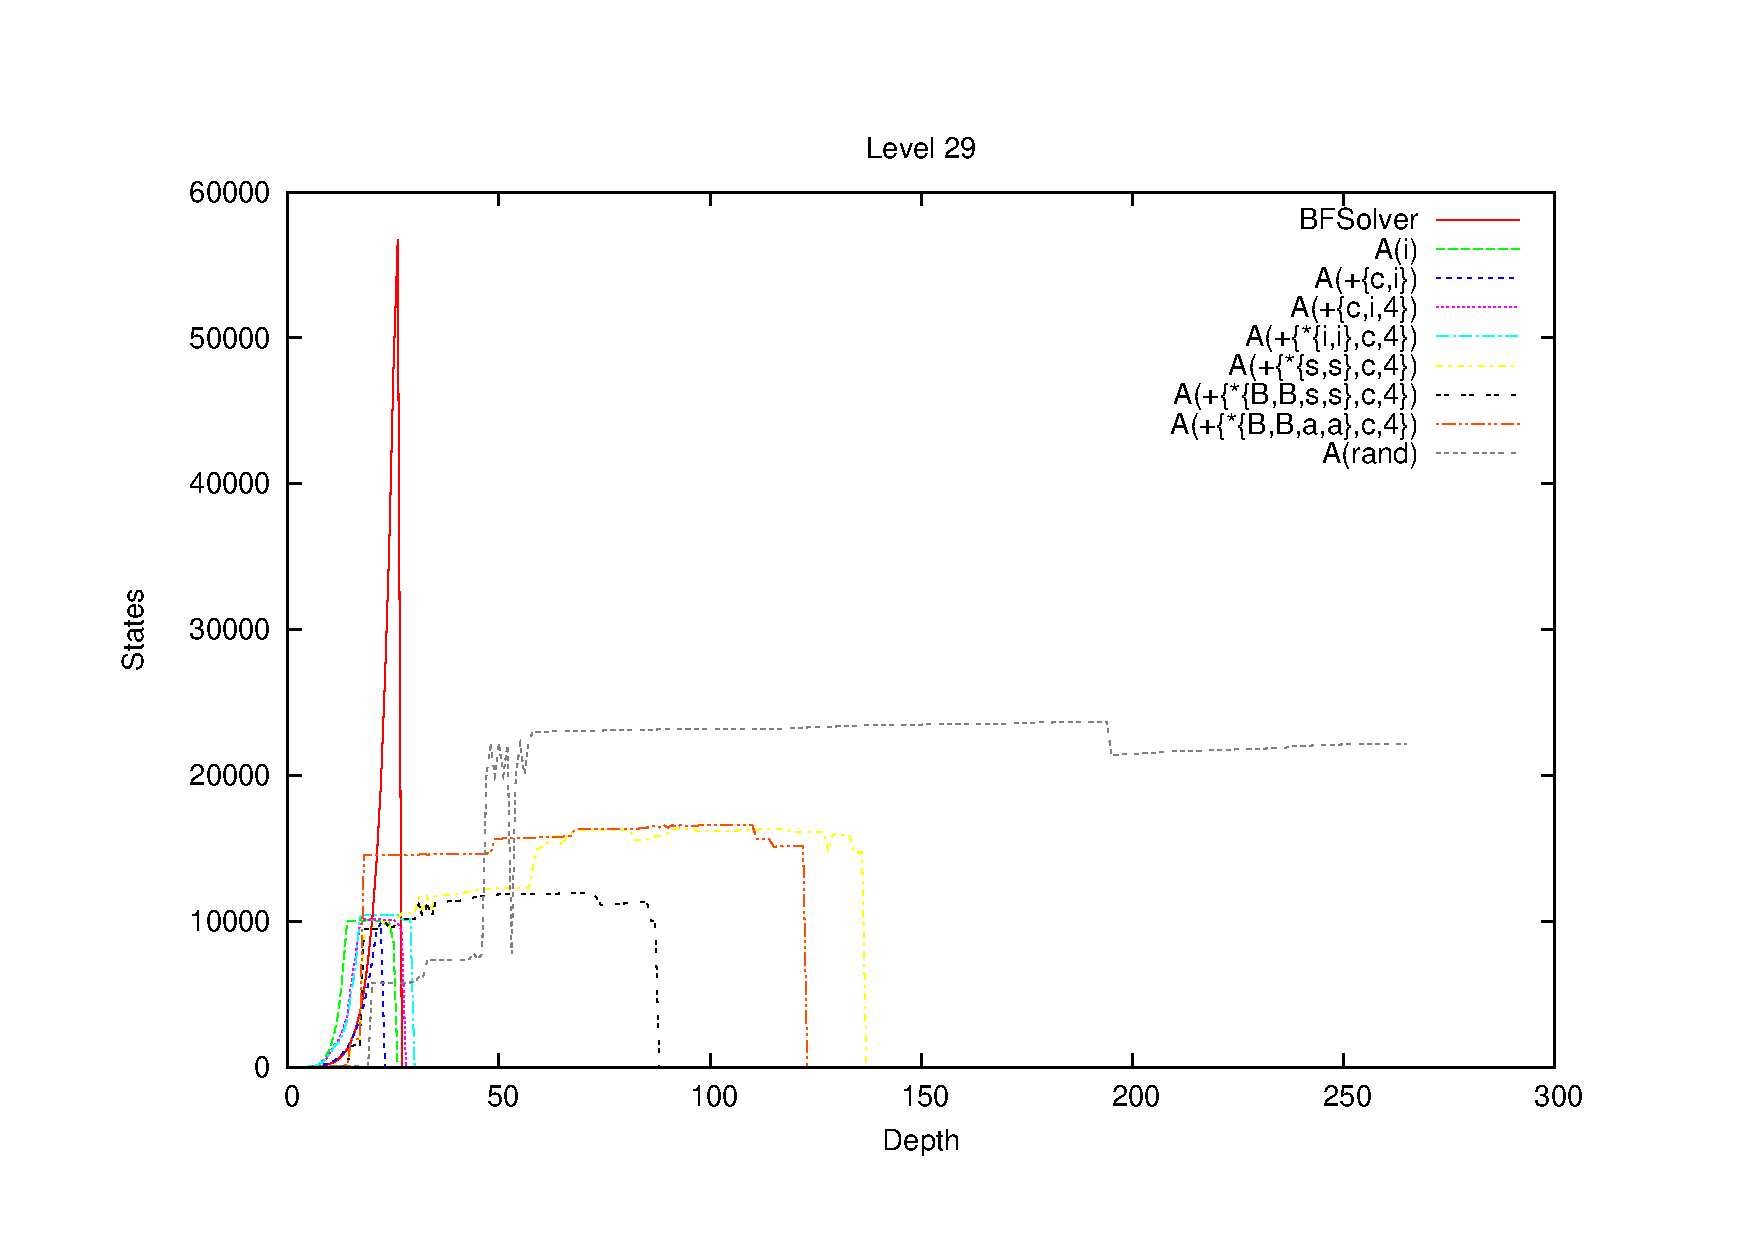
\includegraphics[width=0.85\textwidth]{level29-5}
  \caption{Level 29}
  \label{fig:level29-stats}
\end{figure}
 
\begin{figure}
  \centering
  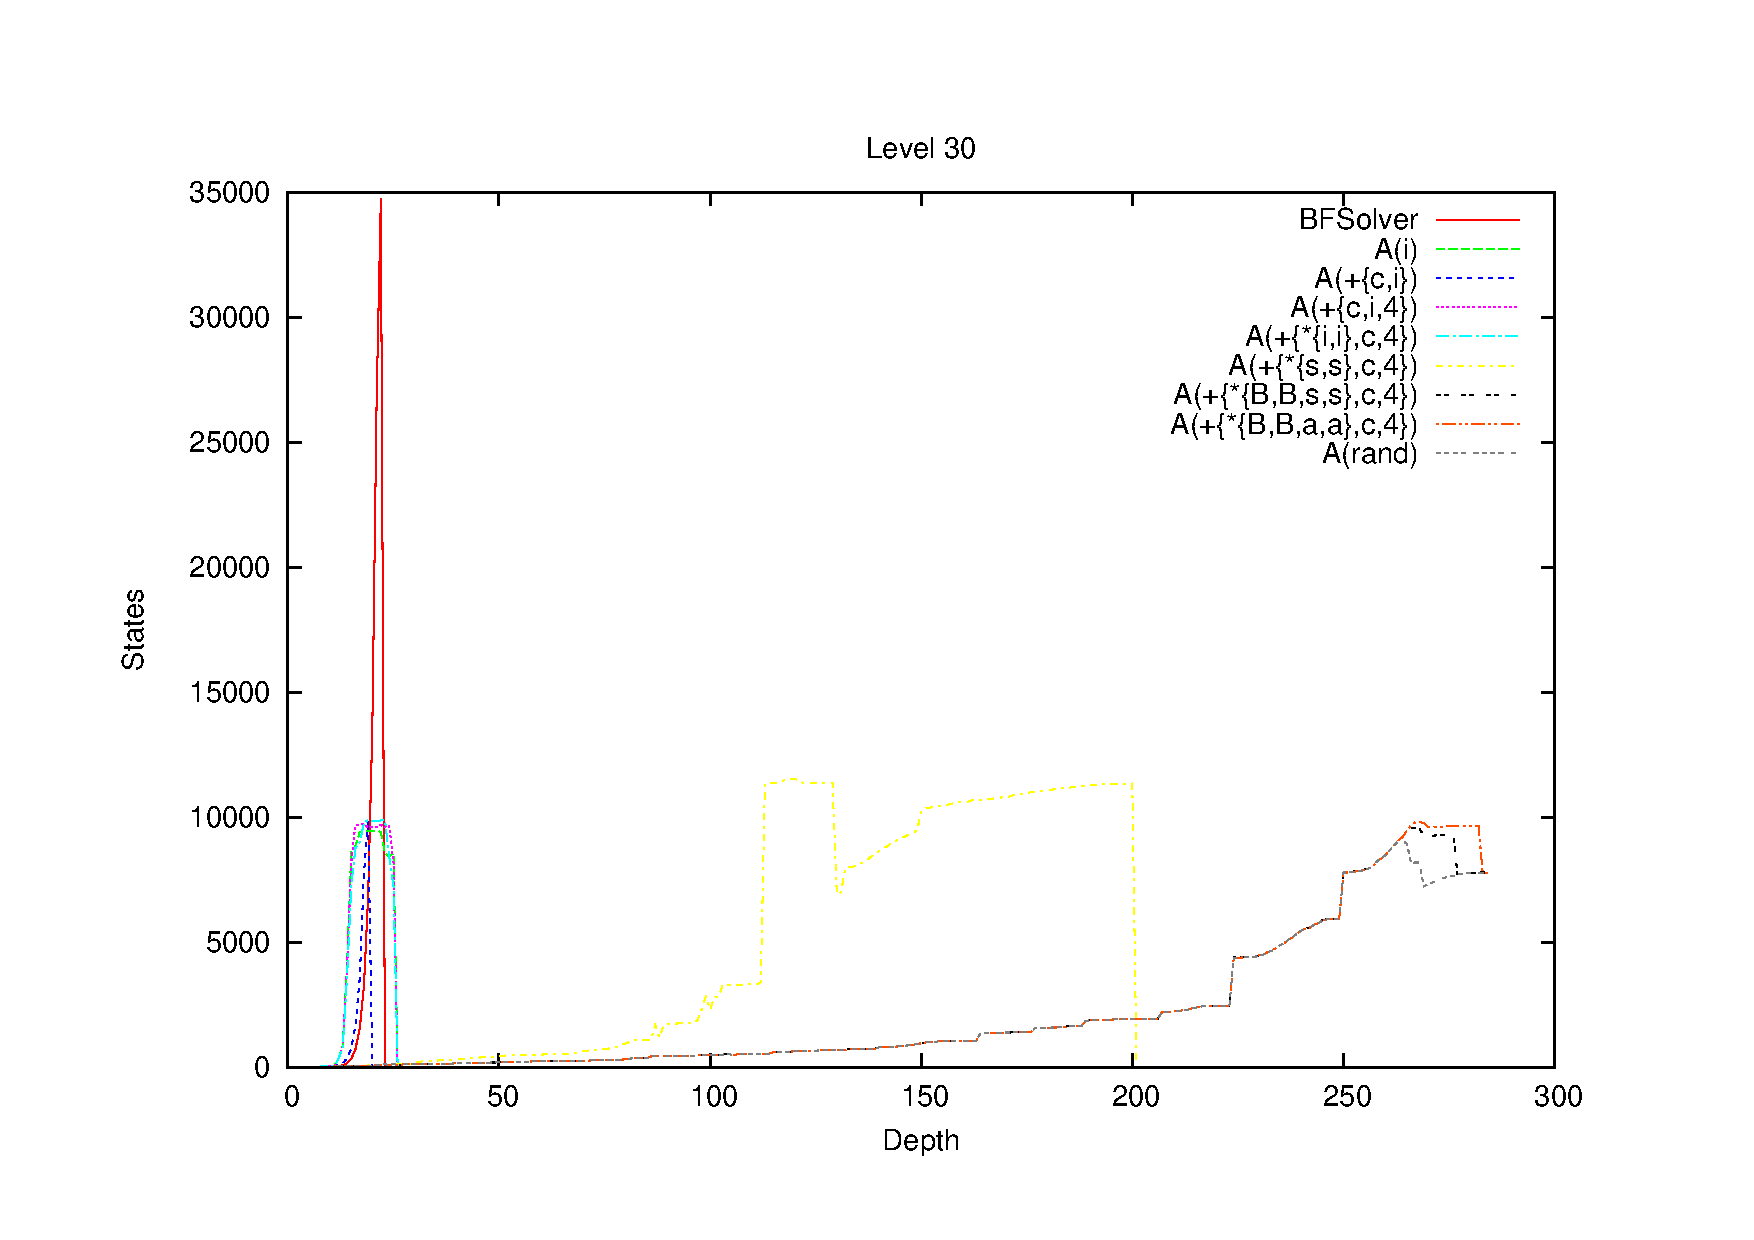
\includegraphics[width=0.85\textwidth]{level30-5}
  \caption{Level 30}
  \label{fig:level30-stats}
\end{figure}

\clearpage

\begin{figure}
  \centering
  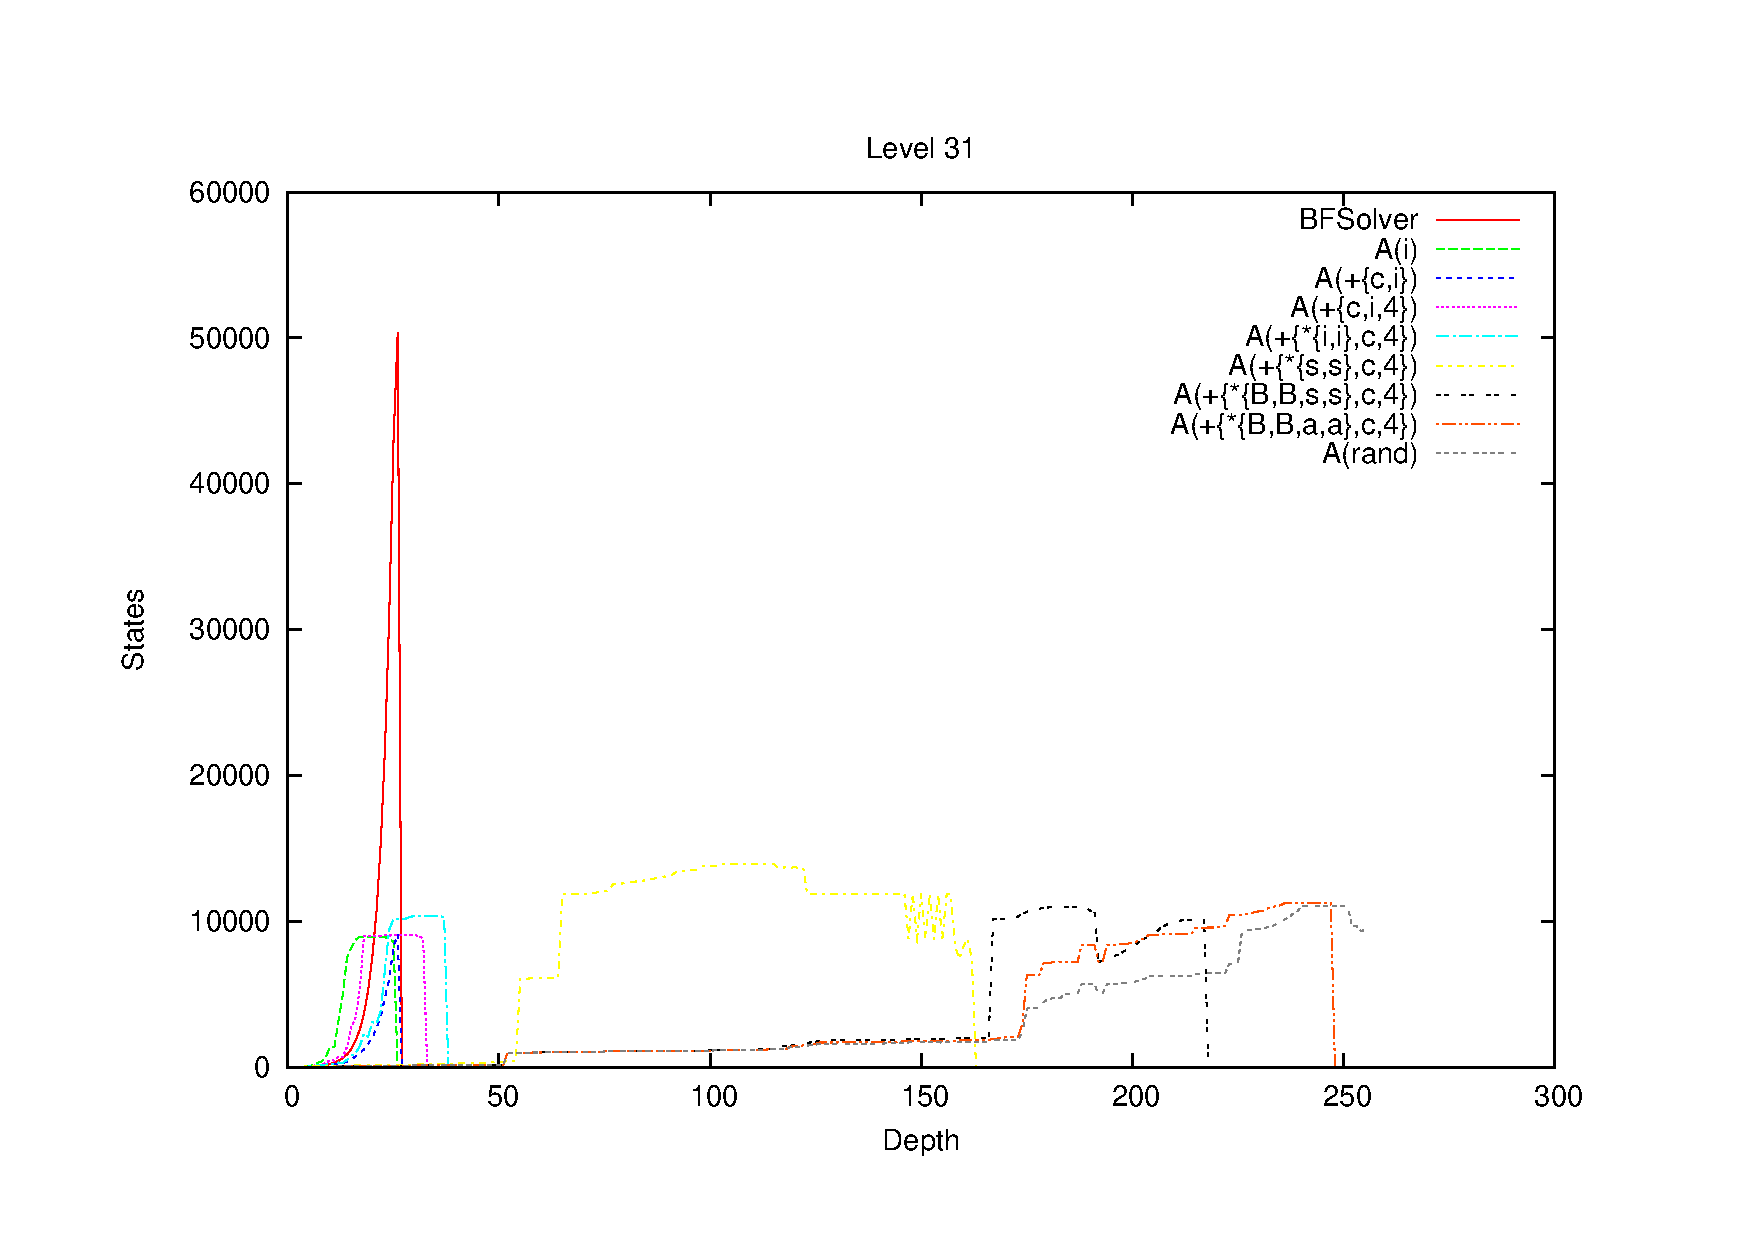
\includegraphics[width=0.85\textwidth]{level31-5}
  \caption{Level 31}
  \label{fig:level31-stats}
\end{figure}
 
\begin{figure}
  \centering
  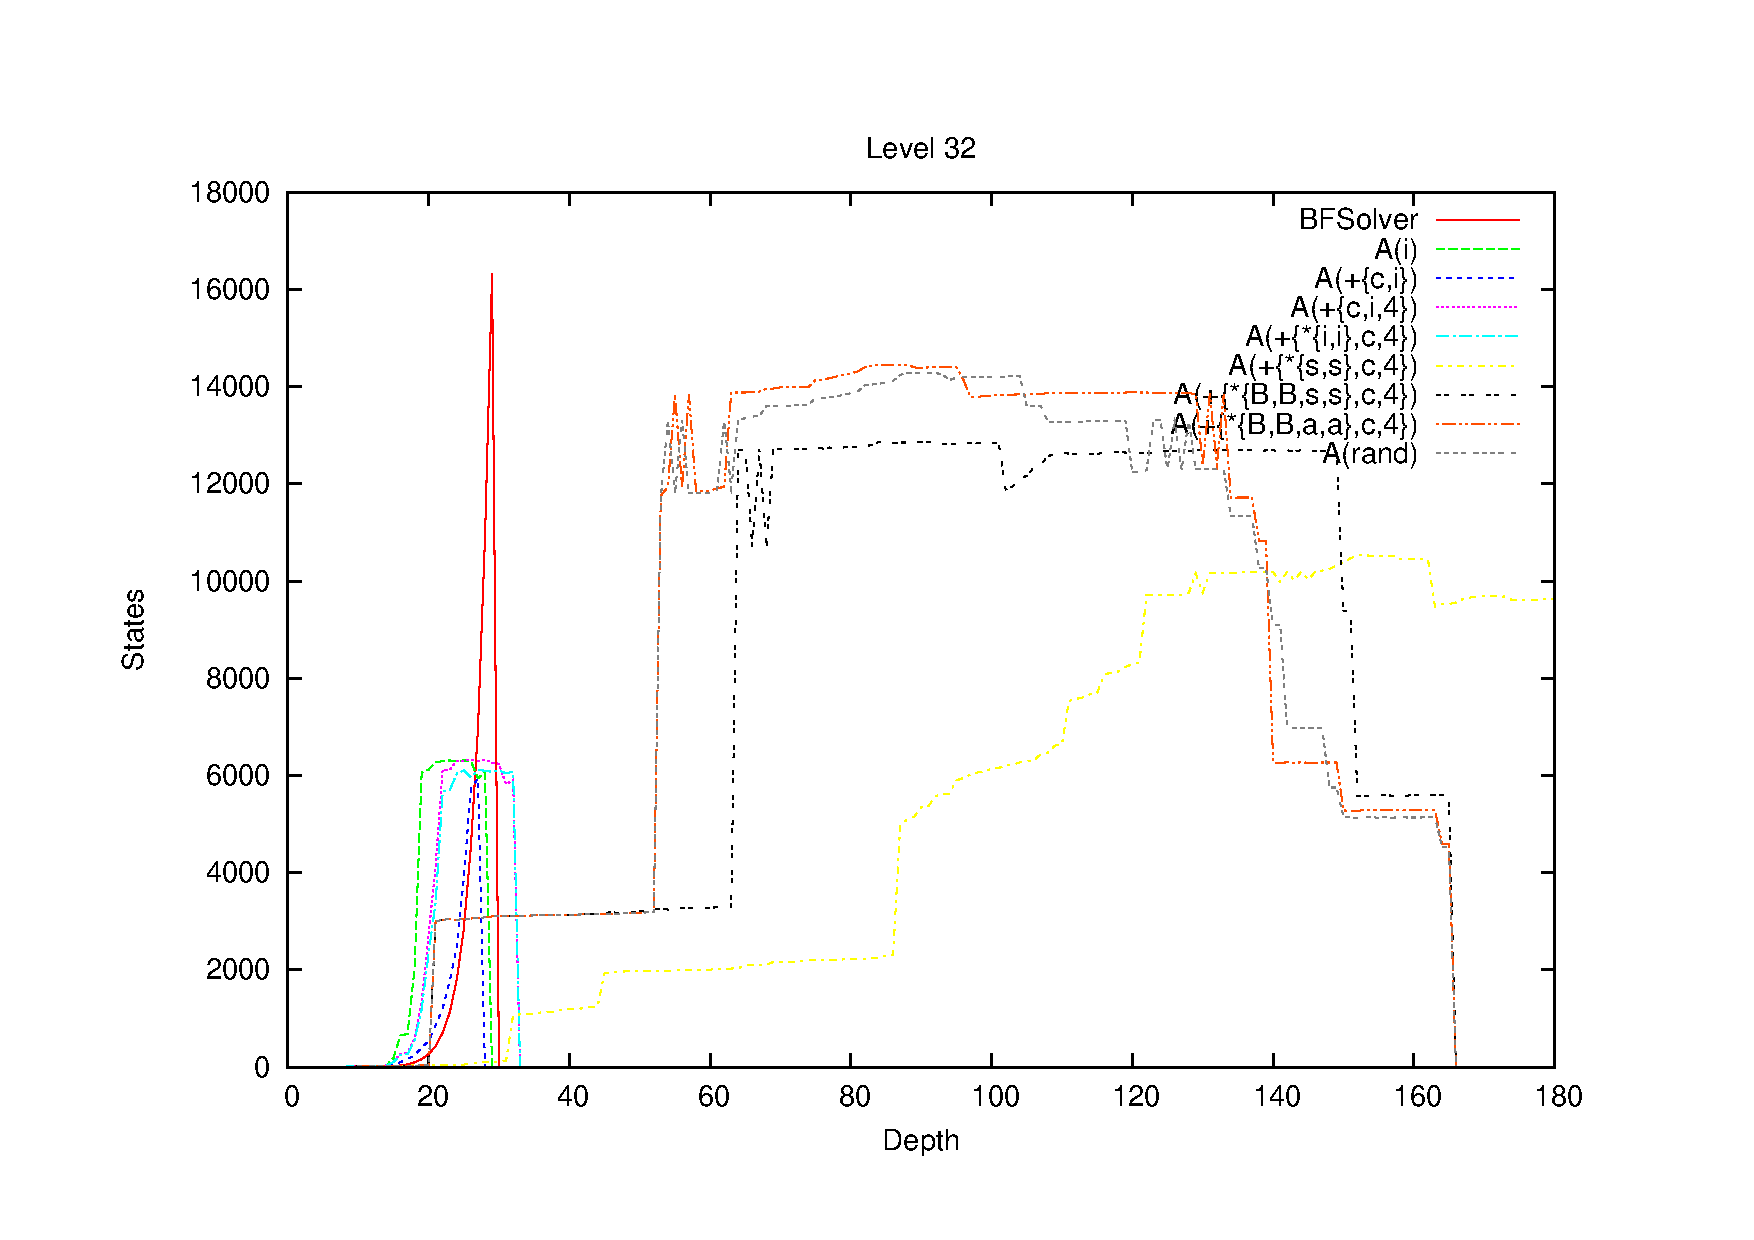
\includegraphics[width=0.85\textwidth]{level32-5}
  \caption{Level 32}
  \label{fig:level32-stats}
\end{figure}

\begin{figure}
  \centering
  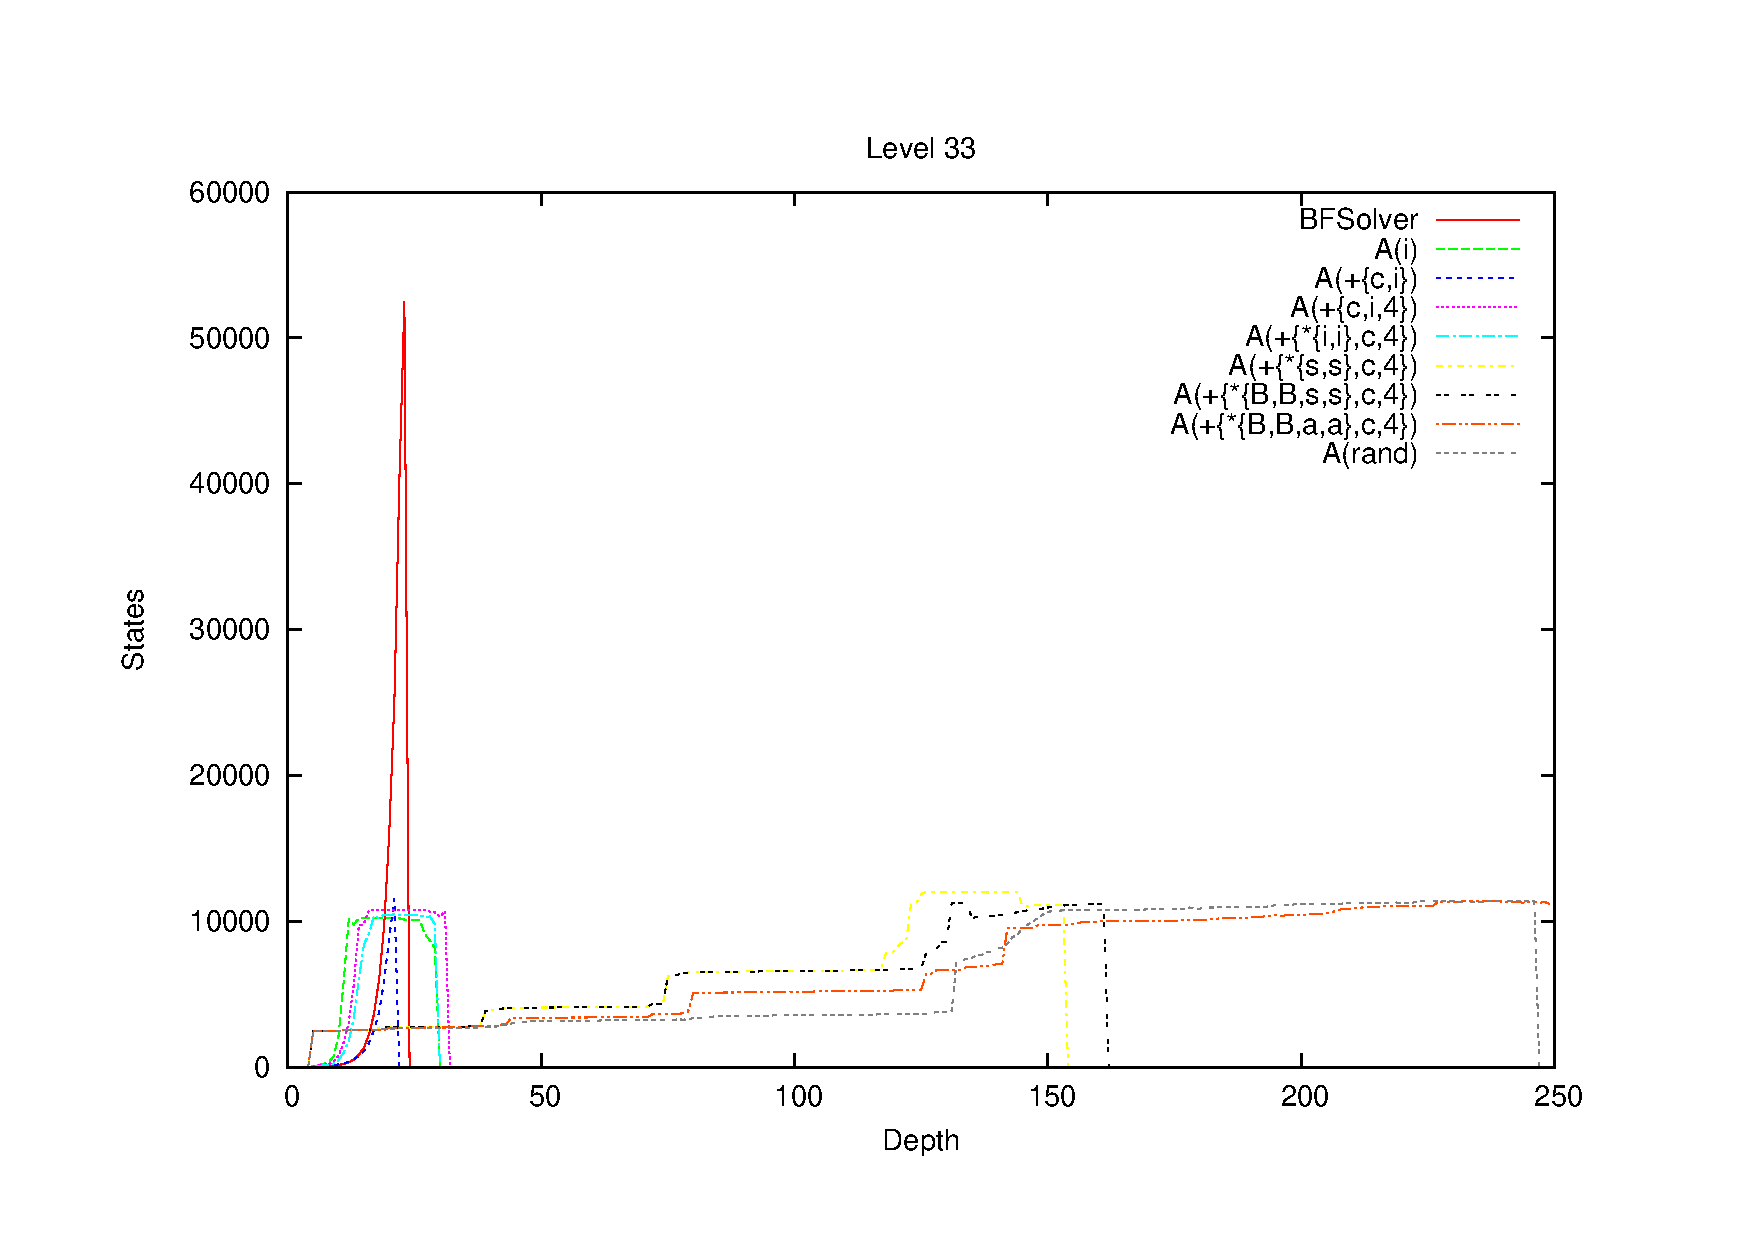
\includegraphics[width=0.85\textwidth]{level33-5}
  \caption{Level 33}
  \label{fig:level33-stats}
\end{figure}
 
\begin{figure}
  \centering
  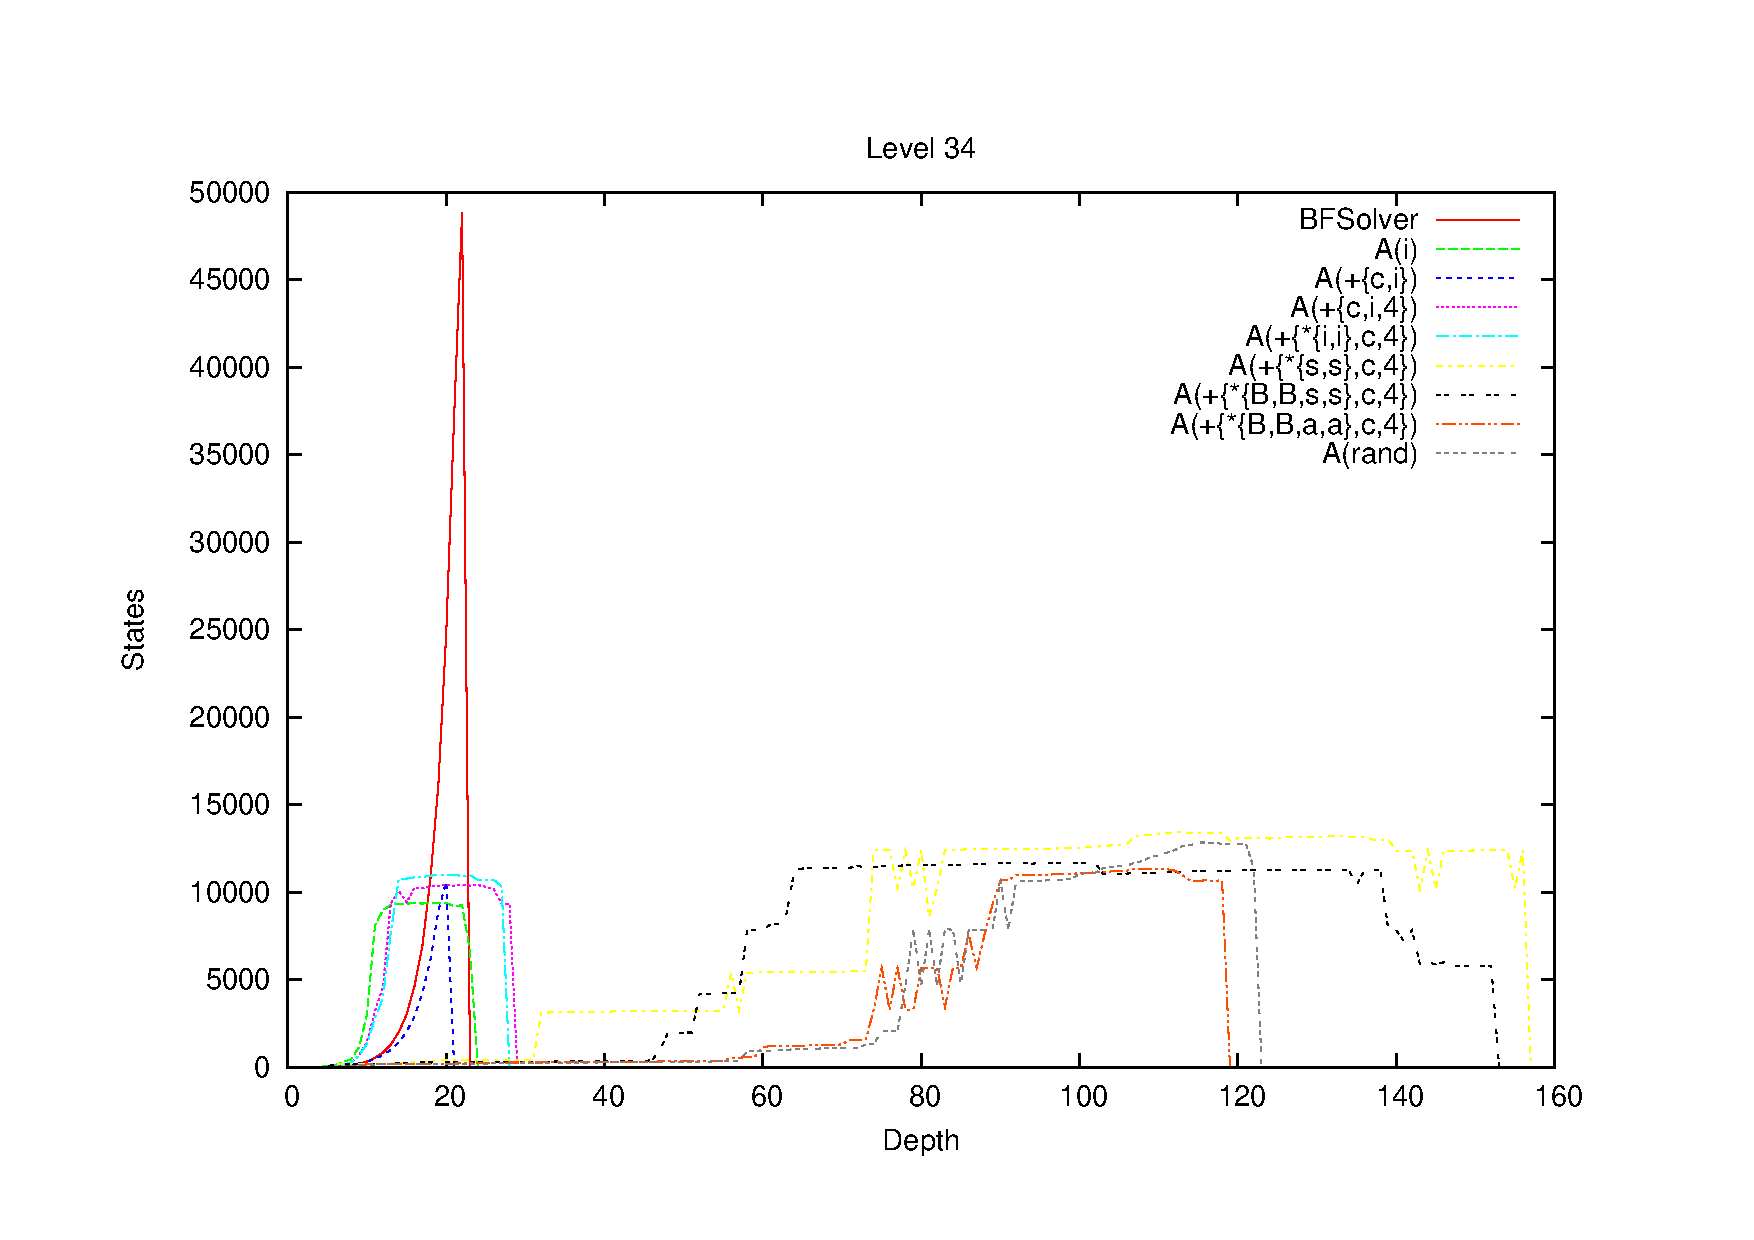
\includegraphics[width=0.85\textwidth]{level34-5}
  \caption{Level 34}
  \label{fig:level34-stats}
\end{figure}

\begin{figure}
  \centering
  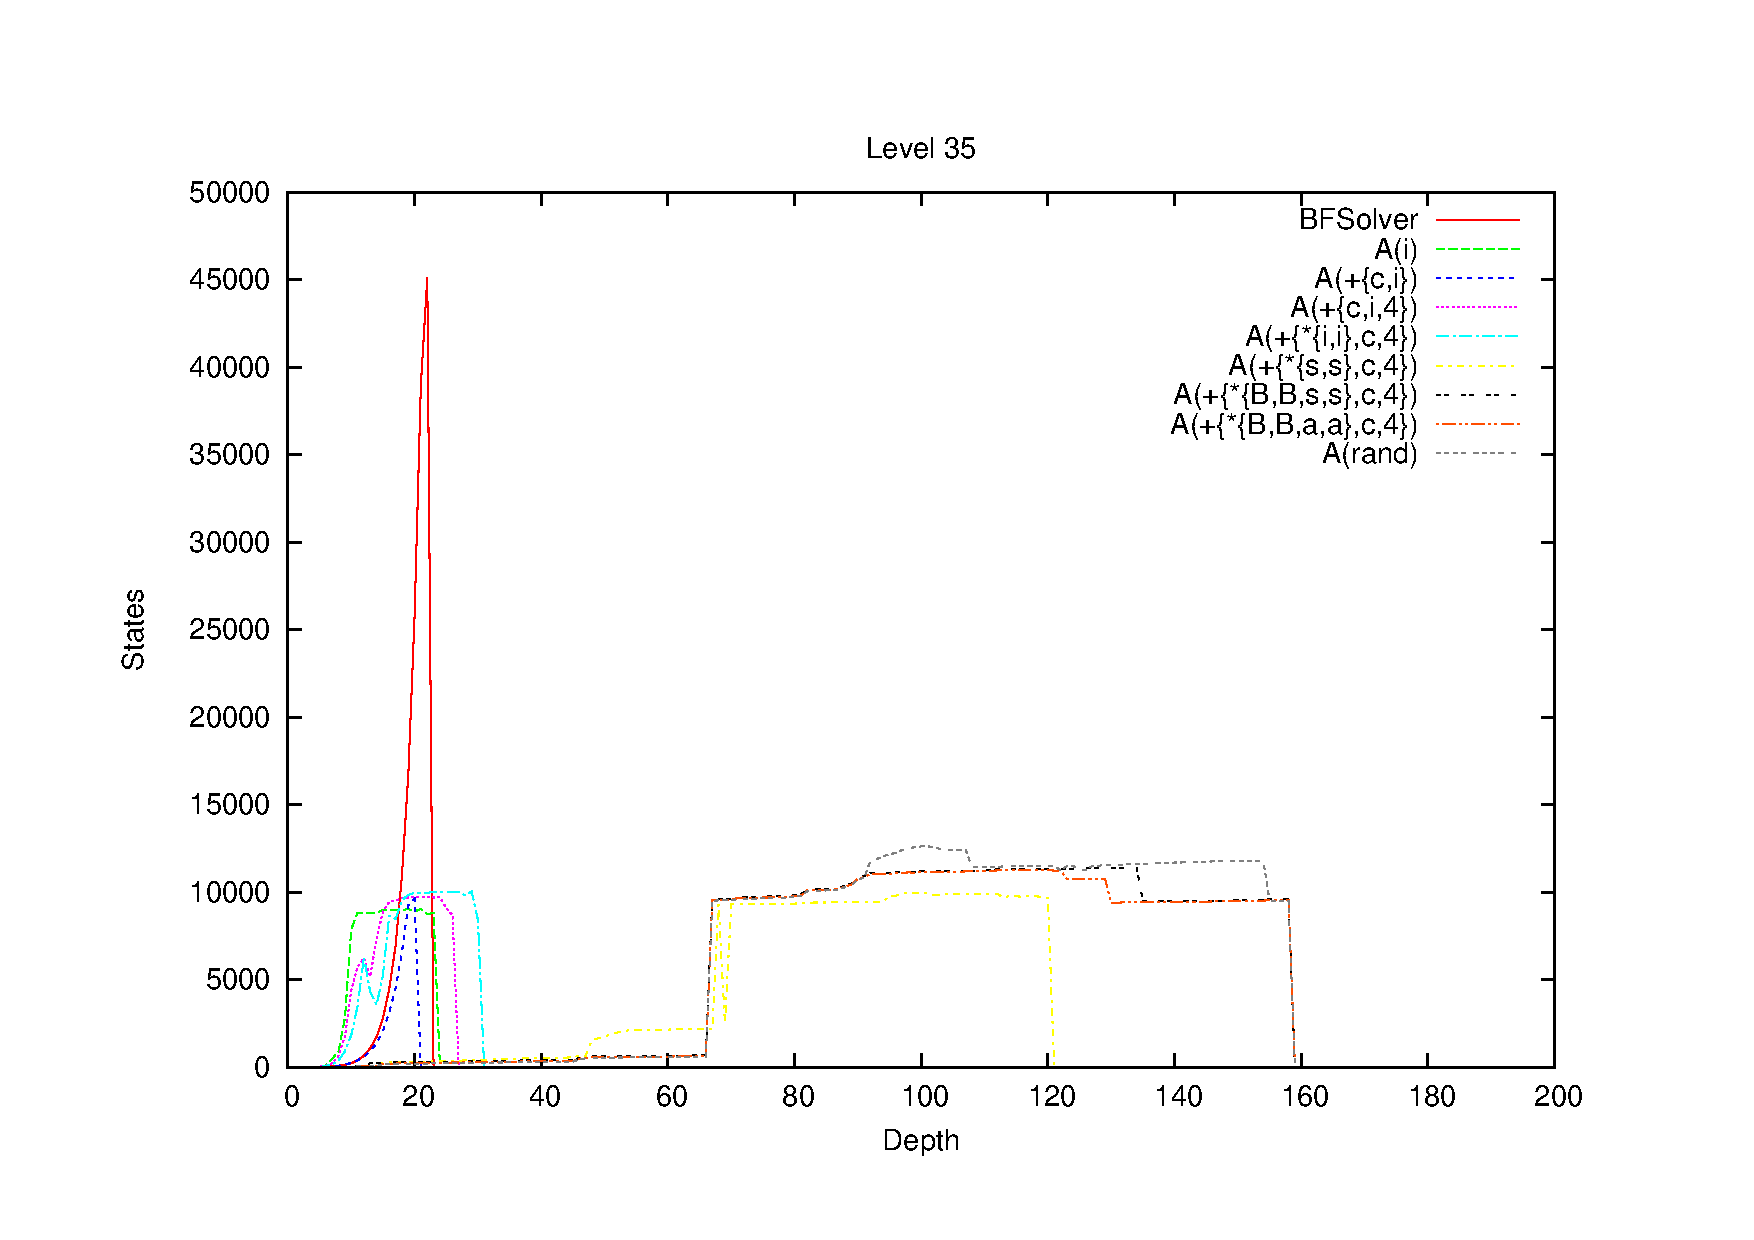
\includegraphics[width=0.85\textwidth]{level35-5}
  \caption{Level 35}
  \label{fig:level35-stats}
\end{figure}
 
\begin{figure}
  \centering
  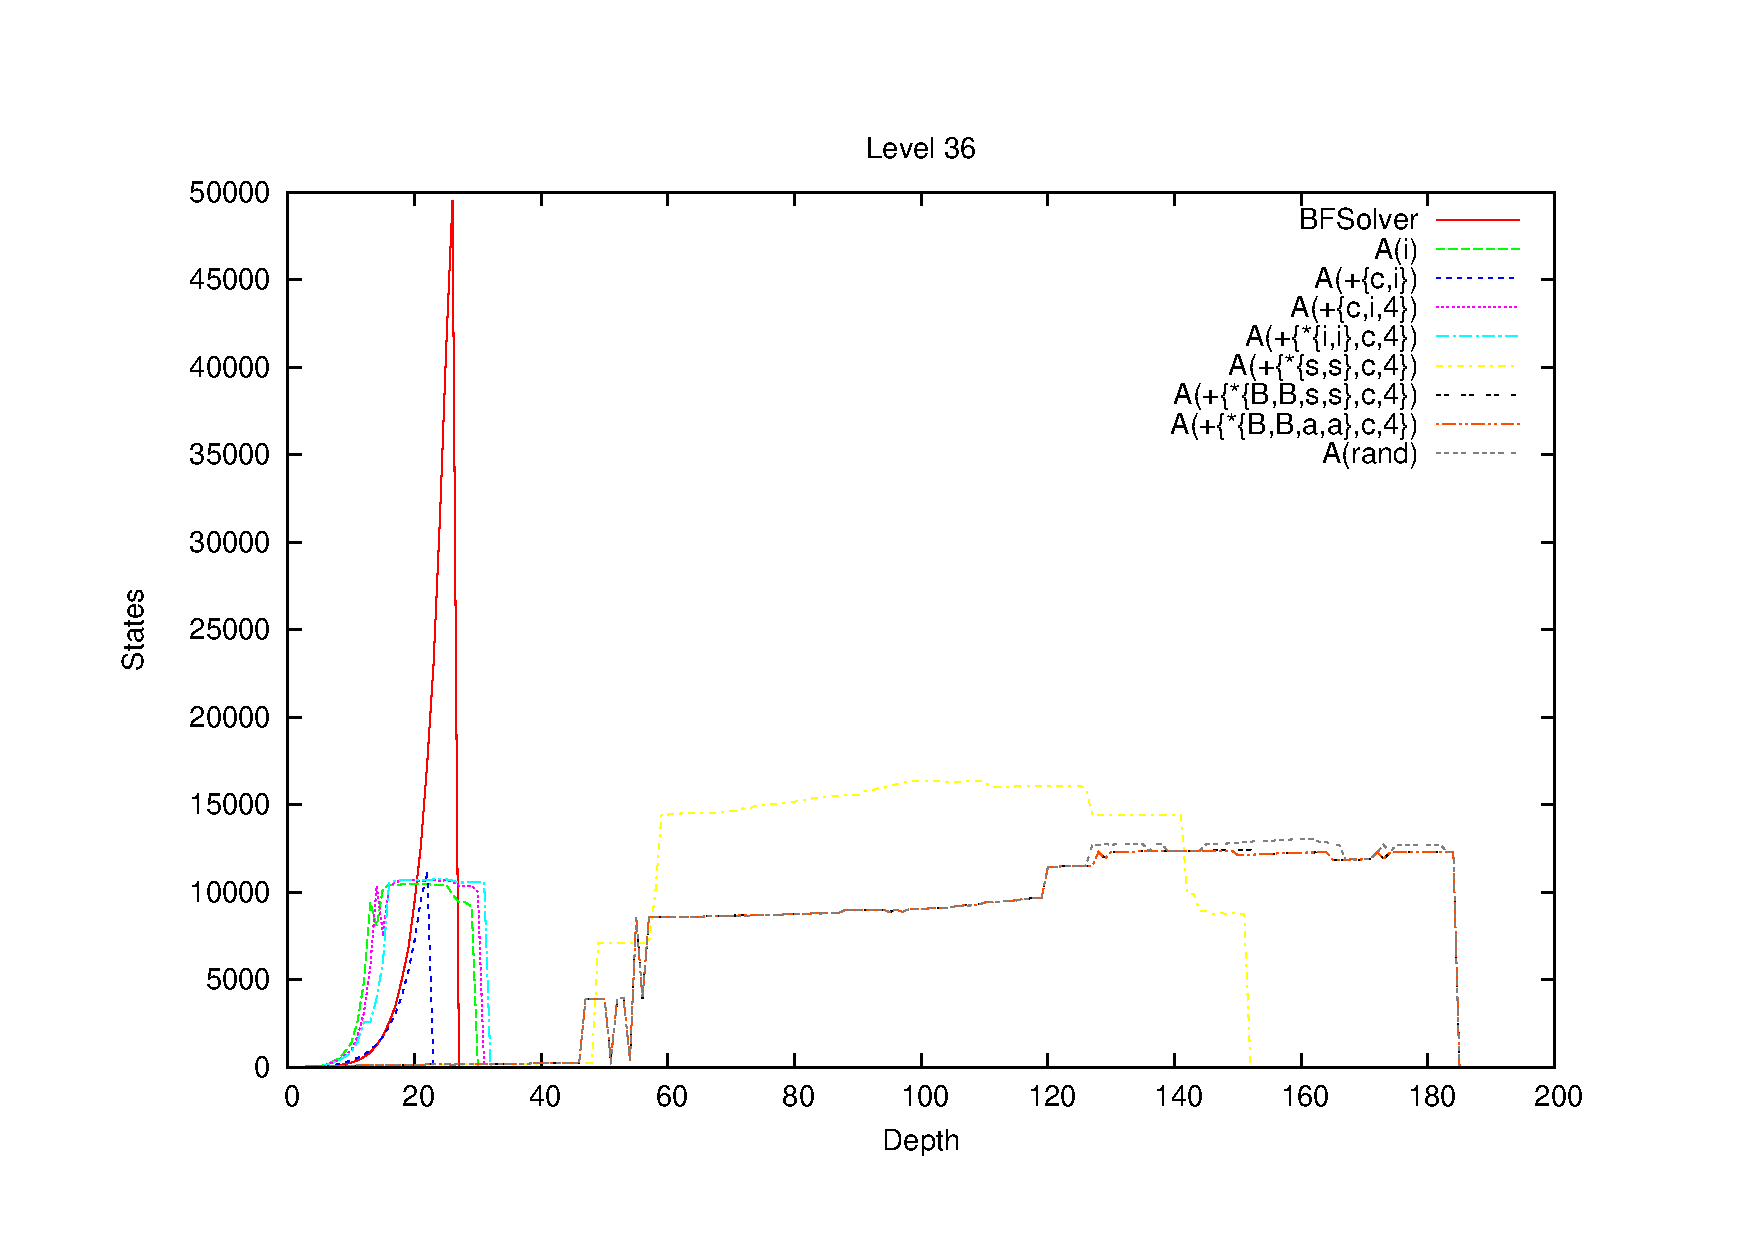
\includegraphics[width=0.85\textwidth]{level36-5}
  \caption{Level 36}
  \label{fig:level36-stats}
\end{figure}

\begin{figure}
  \centering
  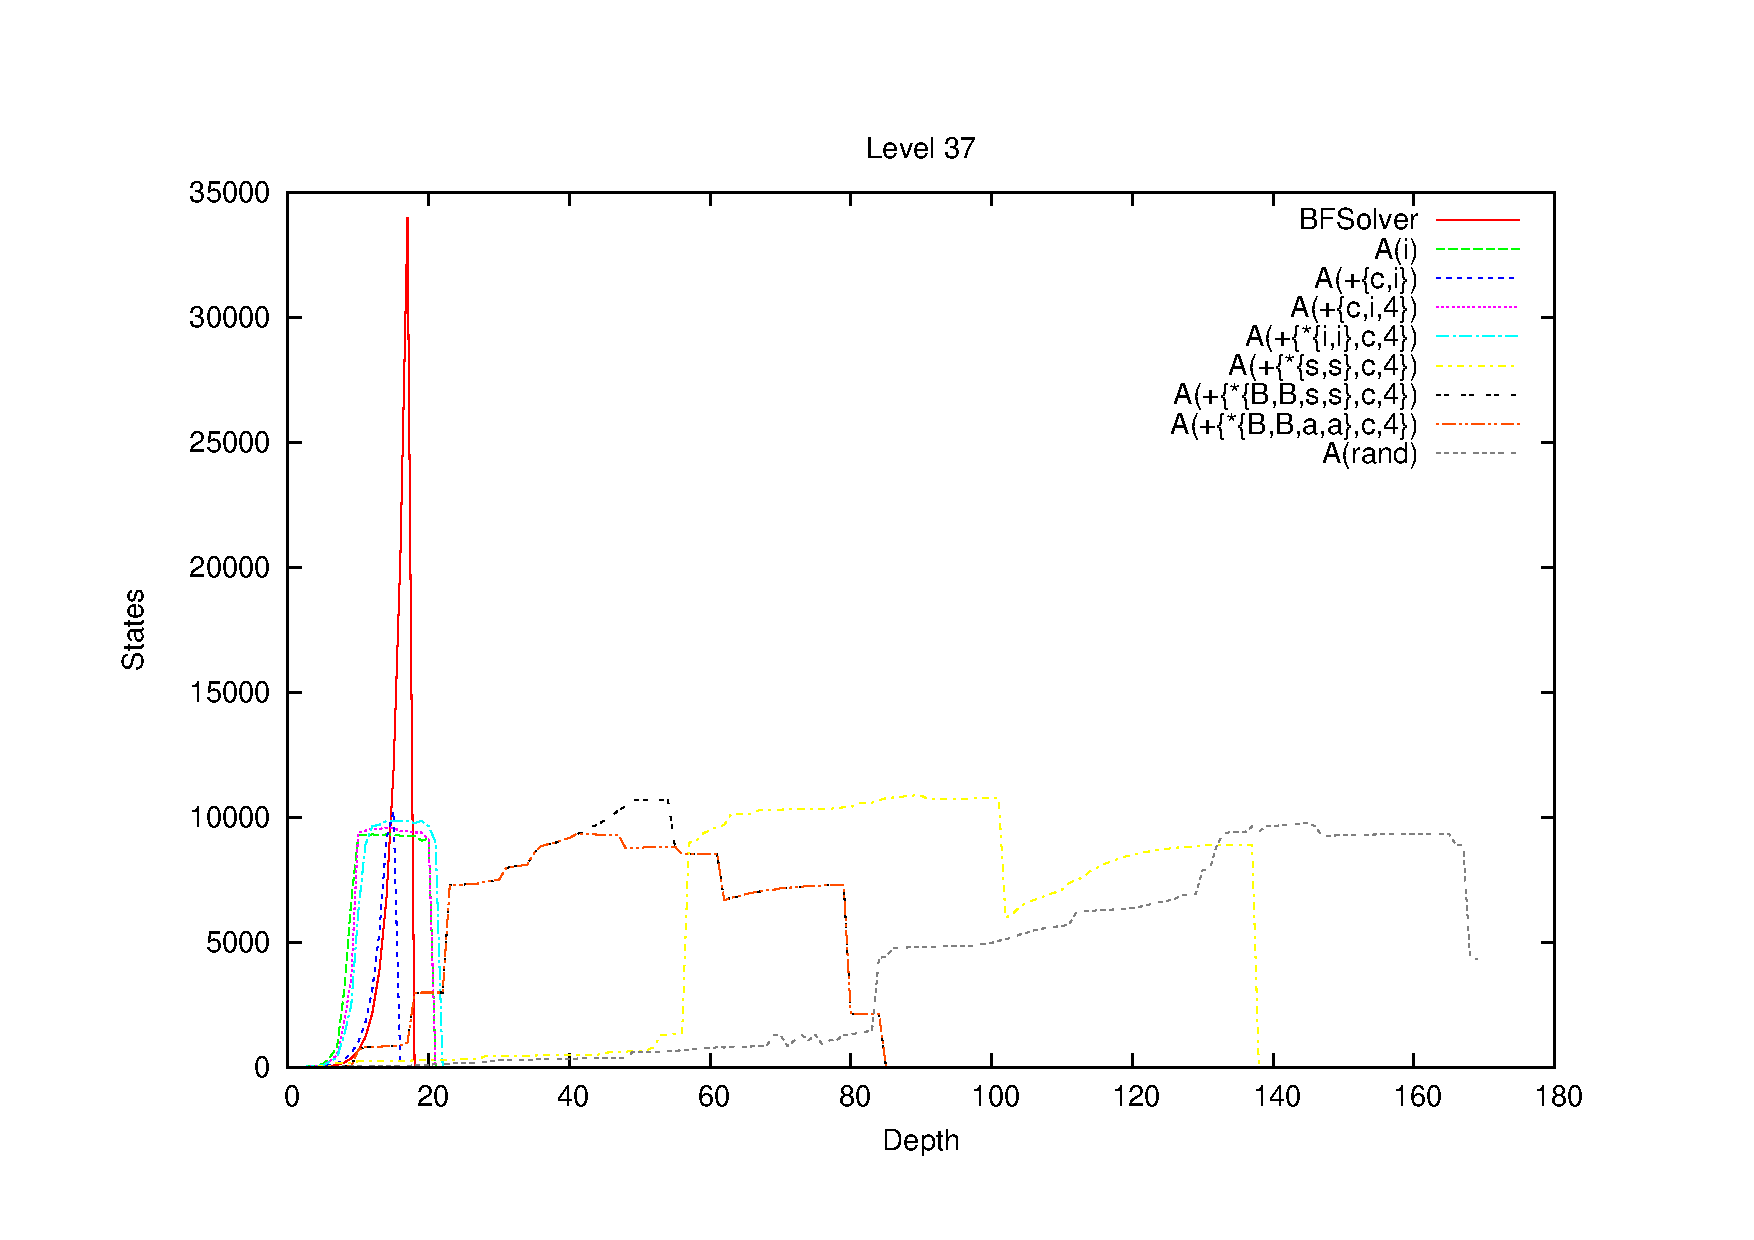
\includegraphics[width=0.85\textwidth]{level37-5}
  \caption{Level 37}
  \label{fig:level37-stats}
\end{figure}
 
\begin{figure}
  \centering
  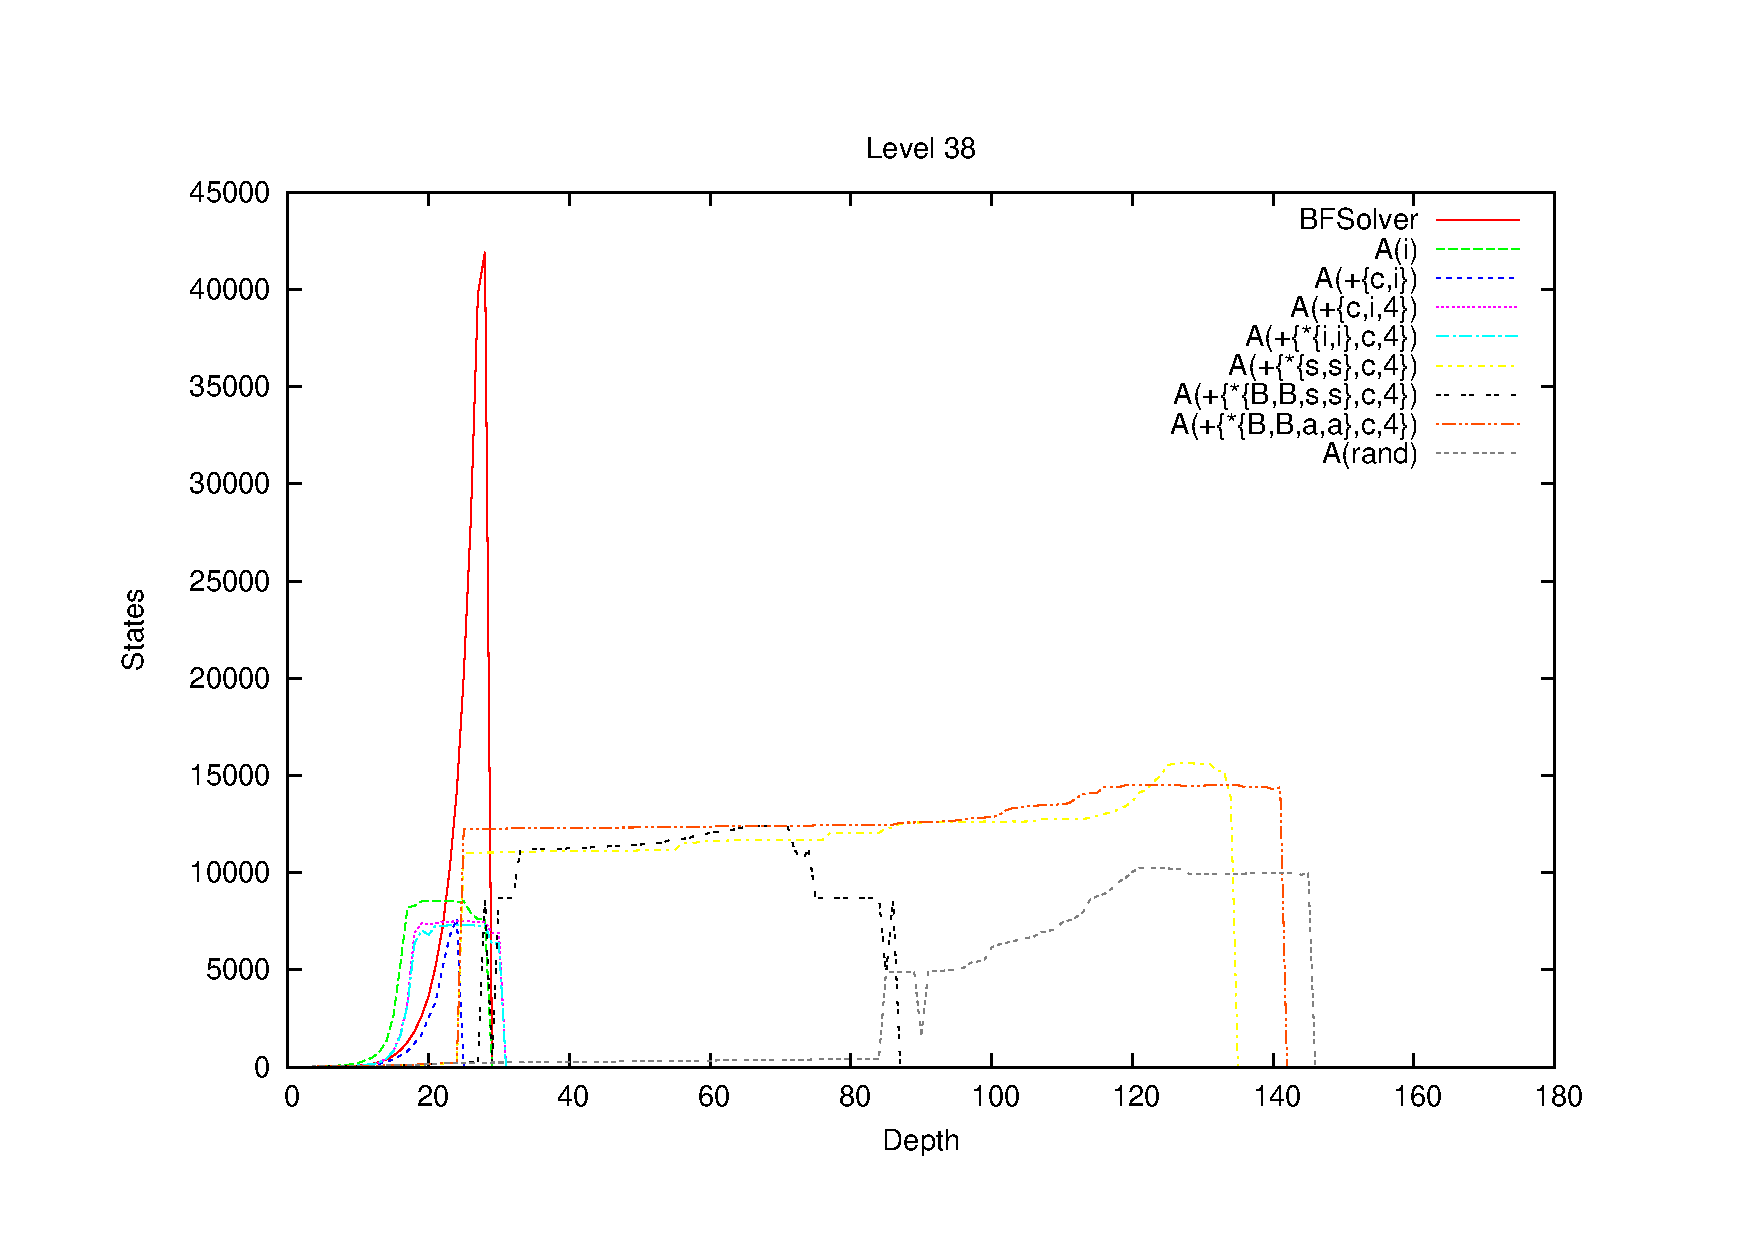
\includegraphics[width=0.85\textwidth]{level38-5}
  \caption{Level 38}
  \label{fig:level38-stats}
\end{figure}

\begin{figure}
  \centering
  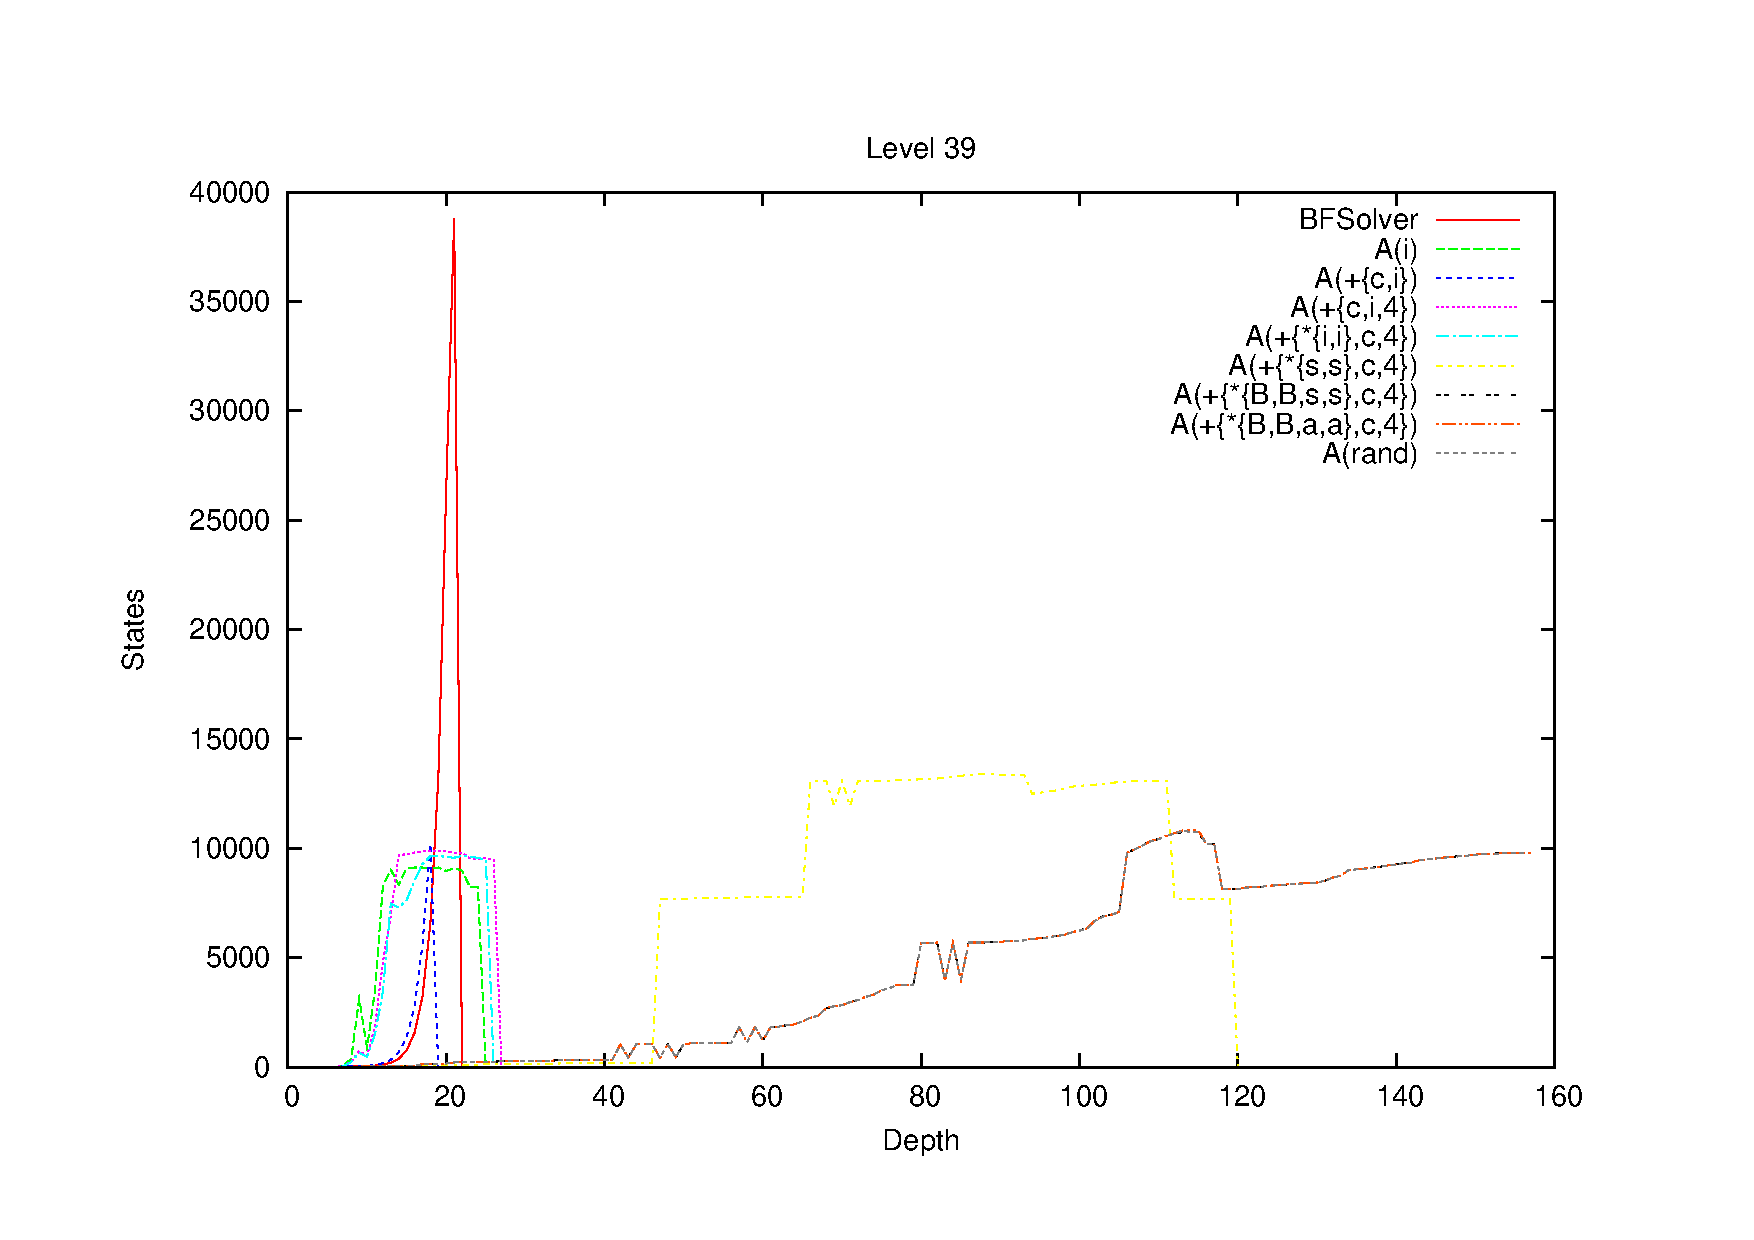
\includegraphics[width=0.85\textwidth]{level39-5}
  \caption{Level 39}
  \label{fig:level39-stats}
\end{figure}
 
\begin{figure}
  \centering
  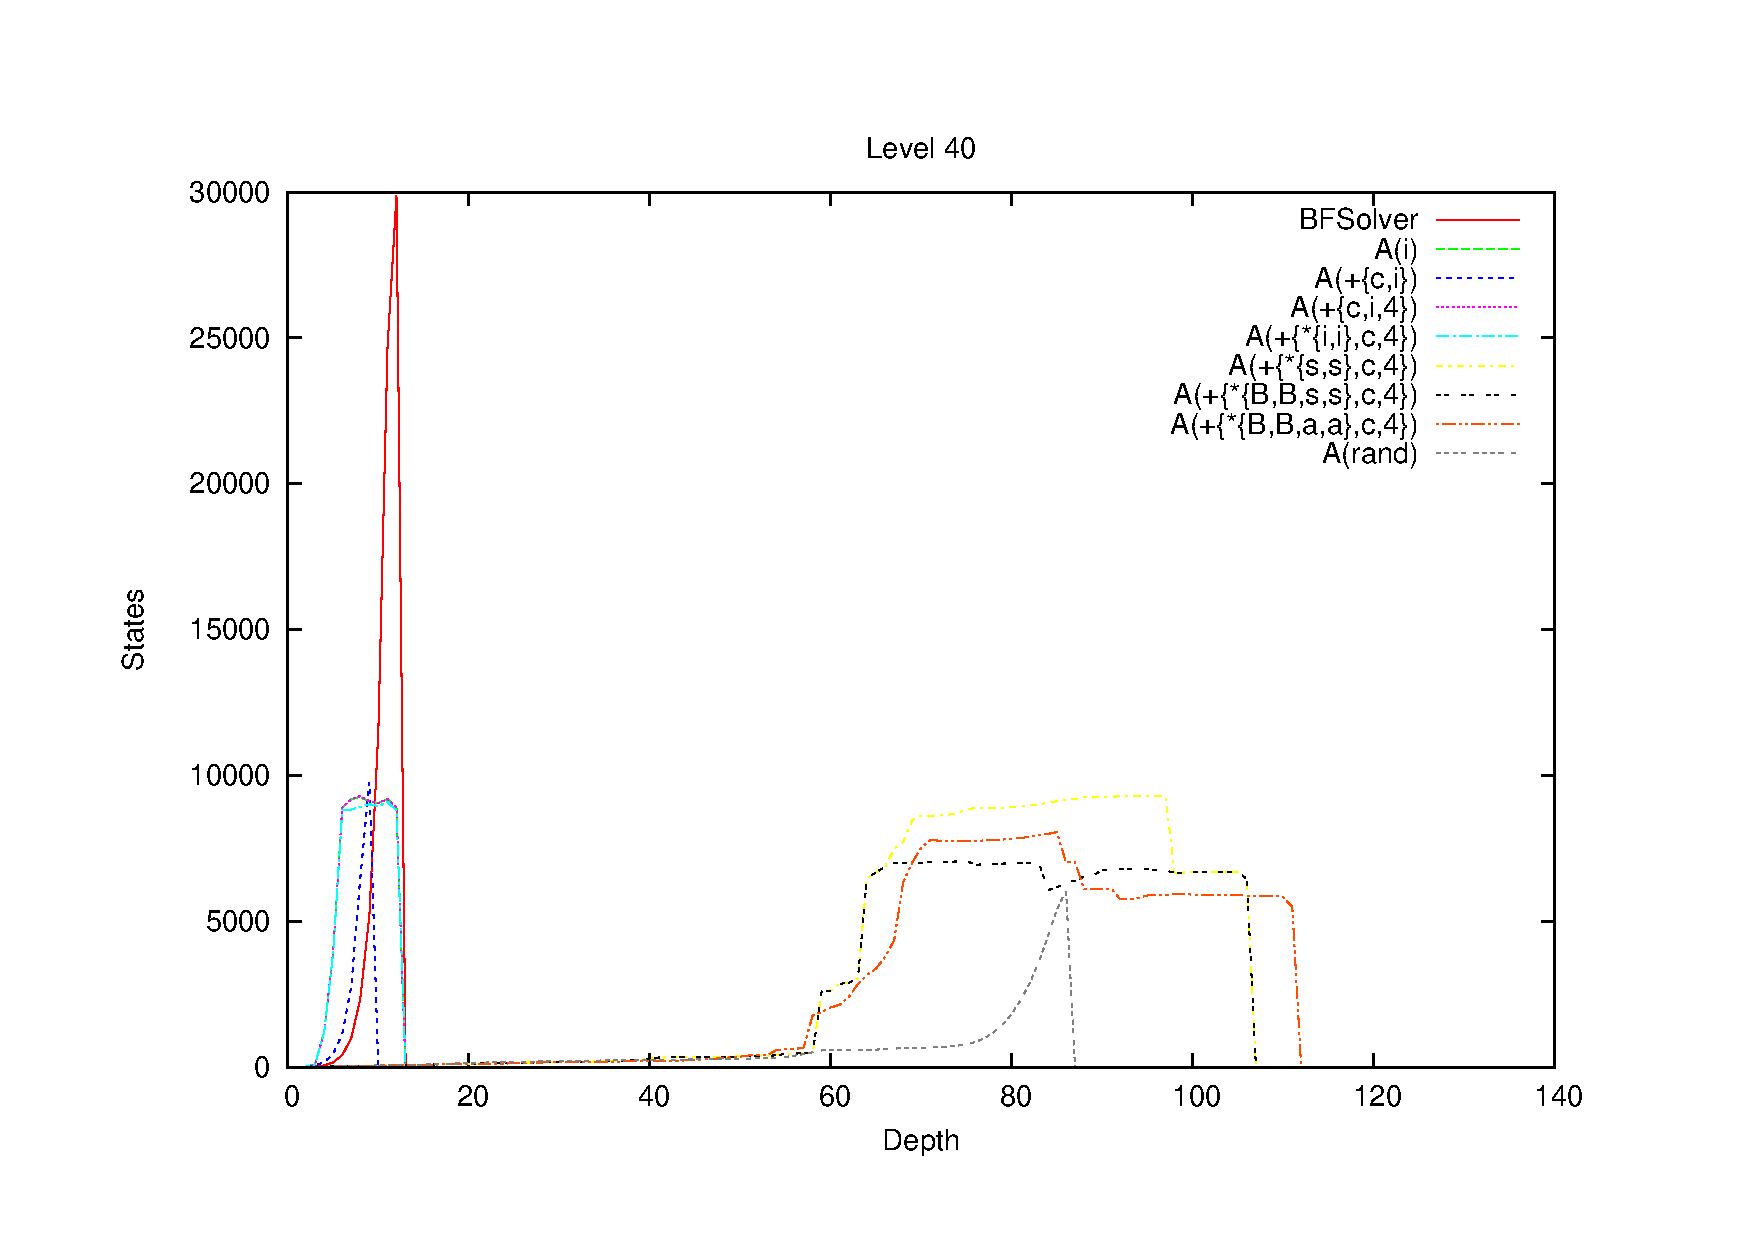
\includegraphics[width=0.85\textwidth]{level40-5}
  \caption{Level 40}
  \label{fig:level40-stats}
\end{figure}

\clearpage
